\documentclass[12pt, a4paper, oneside, openright, titlepage]{book}
\usepackage[utf8]{inputenc}
\raggedbottom
\usepackage{import}


%%%%%%%%%%%%%%%%% Book Formatting Comments:

%%%%%%%%%%%%%%%%%%%%%%%%%%%%%%%%%%%%% for Part

%%%%%%%%%%%%%%%%%%%%%% for chapter

%%%%%%%%%%%%%%%%%%%% for section








%%%%%% PACKAGES %%%%%%%
\usepackage{hyperref}
\hypersetup{
    colorlinks,
    citecolor=black,
    filecolor=black,
    linkcolor=black,
    urlcolor=black
}
\usepackage{amsmath} % Math display options
\usepackage{amssymb} % Math symbols
\usepackage{amsfonts} % Math fonts
\usepackage{amsthm}
\usepackage{mathtools} % General math tools
\usepackage{array} % Allows you to write arrays
\usepackage{empheq} % For boxing equations
\usepackage{mathabx}
\usepackage{mathrsfs}
\usepackage{nameref}

\usepackage{soul}
\usepackage[normalem]{ulem}

\usepackage{txfonts}
\usepackage{cancel}
\usepackage[toc, page]{appendix}
\usepackage{titletoc,tocloft}
\setlength{\cftchapindent}{1em}
\setlength{\cftsecindent}{2em}
\setlength{\cftsubsecindent}{3em}
\setlength{\cftsubsubsecindent}{4em}
\usepackage{titlesec}

\titleformat{\section}
  {\normalfont\fontsize{25}{15}\bfseries}{\thesection}{1em}{}
\titleformat{\section}
  {\normalfont\fontsize{20}{15}\bfseries}{\thesubsection}{1em}{}
\setcounter{secnumdepth}{1}  
  
  

\newcommand\numberthis{\refstepcounter{equation}\tag{\theequation}} % For equation labelling
\usepackage[framemethod=tikz]{mdframed}

\usepackage{tikz} % For drawing commutative diagrams
\usetikzlibrary{cd}
\usetikzlibrary{calc}
\tikzset{every picture/.style={line width=0.75pt}} %set default line width to 0.75p

\usepackage{datetime}
\usepackage[margin=1in]{geometry}
\setlength{\parskip}{1em}
\usepackage{graphicx}
\usepackage{float}
\usepackage{fancyhdr}
\setlength{\headheight}{15pt} 
\pagestyle{fancy}
\lhead[\leftmark]{}
\rhead[]{\leftmark}

\usepackage{enumitem}

\usepackage{url}
\allowdisplaybreaks

%%%%%% ENVIRONMENTS %%%
\definecolor{purp}{rgb}{0.29, 0, 0.51}
\definecolor{bloo}{rgb}{0, 0.13, 0.80}



%%\newtheoremstyle{note}% hnamei
%{3pt}% hSpace above
%{3pt}% hSpace belowi
%{}% hBody fonti
%{}% hIndent amounti
%{\itshape}% hTheorem head fonti
%{:}% hPunctuation after theorem headi
%{.5em}% hSpace after theorem headi
%{}% hTheorem head spec (can be left empty, meaning ‘normal’)i


%%%%%%%%%%%%% THEOREM STYLES

\newtheoremstyle{BigTheorem}
{20pt}
{20pt}
{\slshape}
{}
{\Large\color{purp}\bfseries}
{.}
{\newline}
{\thmname{#1}\thmnumber{ #2}\thmnote{ (#3)}}



\newtheoremstyle{TheoremClassic}
{15pt}
{15pt}
{\slshape}
{}
{\bfseries}
{.}
{.5em}
{}

\newtheoremstyle{Definitions}
{15pt}
{15pt}
{\slshape}
{}
{\bfseries}
{.}
{.5em}
{\thmname{#1}\thmnumber{ #2}\thmnote{ (#3)}}


\newtheoremstyle{Remarks}
{10pt}
{10pt}
{\upshape}
{}
{\bfseries}
{.}
{.5em}
{}

\newtheoremstyle{Examples}
{10pt}
{10pt}
{\upshape}
{}
{\bfseries}
{.}
{.5em}
{}


%%%%%%%%%%%%% THEOREM DEFINITIONS

\theoremstyle{BigTheorem}
\newtheorem{namthm}{Theorem}
\newtheorem{conj}[namthm]{Conjecture}

\theoremstyle{TheoremClassic}
\newtheorem{thm}{Theorem}[section]
\newtheorem*{thm*}{Theorem}
\newtheorem{lem}[thm]{Lemma}
\newtheorem{cor}[thm]{Corollary}
\newtheorem{prop}[thm]{Proposition}
\newtheorem{claim}[thm]{Claim}


\theoremstyle{Definitions}
\newtheorem{defn}{Definition}[section]
\newtheorem{axi}[defn]{Axiom}
\newtheorem{cust}[defn]{}
\newtheorem{cons}[defn]{Construction}
\newtheorem{props}[defn]{Properties}
\newtheorem{proc}[defn]{Process}
\newtheorem*{law}{Law}


\theoremstyle{Examples}
\newtheorem{eg}{Example}[section]
\newtheorem{noneg}[eg]{Non-Example}
\newtheorem{xca}[eg]{Exercise}


\theoremstyle{Remarks}
\newtheorem{rmk}{Remark}[section]
\newtheorem{qst}[rmk]{Question}
\newtheorem*{ans}{Answer}
\newtheorem{obs}[rmk]{Observation}
\newtheorem{rec}[rmk]{Recall}
\newtheorem{summ}[rmk]{Summary}
\newtheorem{nota}[rmk]{Notation}
\newtheorem{note}[rmk]{Note}



\renewcommand{\qedsymbol}{$\blacksquare$}


\numberwithin{equation}{section}

\newenvironment{qest}{
    \begin{center}
        \em
    }
    {
    \end{center}
    }

%%%%%% MACROS %%%%%%%%%
%% New Commands
\newcommand{\ip}[1]{\langle#1\rangle} %%% Inner product
\newcommand{\abs}[1]{\lvert#1\rvert} %%% Modulus
\newcommand\diag{\operatorname{diag}} %%% diag matrix
\newcommand\tr{\mbox{tr}\.} %%% trace
\newcommand\C{\mathbb C} %%% Complex numbers
\newcommand\R{\mathbb R} %%% Real numbers
\newcommand\Z{\mathbb Z} %%% Integers
\newcommand\Q{\mathbb Q} %%% Rationals
\newcommand\N{\mathbb N} %%% Naturals
\newcommand\F{\mathbb F} %%% An arbitrary field
\newcommand\ste{\operatorname{St}} %%% Steinberg Representation
\newcommand\GL{\mathbf{GL}} %%% General Linear group
\newcommand\SL{\mathbf{SL}} %%% Special linear group
\newcommand\gl{\mathfrak{gl}} %%% General linear algebra
\newcommand\G{\mathbf{G}} %%% connected reductive group
\newcommand\g{\mathfrak{g}} %%% Lie algebra of G
\newcommand\Hbf{\mathbf{H}} %%% Theta fixed points of G
\newcommand\X{\mathbf{X}} %%% Symmetric space X
\newcommand{\catname}[1]{\normalfont\textbf{#1}}
\newcommand{\Set}{\catname{Set}} %%% Category set
\newcommand{\Grp}{\catname{Grp}} %%% Category group
\newcommand{\Rmod}{\catname{R-Mod}} %%% Category r-modules
\newcommand{\Mon}{\catname{Mon}} %%% Category monoid
\newcommand{\Ring}{\catname{Ring}} %%% Category ring
\newcommand{\Topp}{\catname{Top}} %%% Category Topological spaces
\newcommand{\Vect}{\catname{Vect}_{k}} %%% category vector spaces'
\newcommand\Hom{\mathbf{Hom}} %%% Arrows

\newcommand{\map}[2]{\begin{array}{c} #1 \\ #2 \end{array}}

\newcommand{\Emph}[1]{\textbf{\ul{\emph{#1}}}}

\newcommand{\mapsfrom}{\mathrel{\reflectbox{\ensuremath{\mapsto}}}}


%% Math operators
\DeclareMathOperator{\ran}{Im} %%% image
\DeclareMathOperator{\aut}{Aut} %%% Automorphisms
\DeclareMathOperator{\spn}{span} %%% span
\DeclareMathOperator{\ann}{Ann} %%% annihilator
\DeclareMathOperator{\rank}{rank} %%% Rank
\DeclareMathOperator{\ch}{char} %%% characteristic
\DeclareMathOperator{\ev}{\bf{ev}} %%% evaluation
\DeclareMathOperator{\sgn}{sign} %%% sign
\DeclareMathOperator{\id}{Id} %%% identity
\DeclareMathOperator{\supp}{Supp} %%% support
\DeclareMathOperator{\inn}{Inn} %%% Inner aut
\DeclareMathOperator{\en}{End} %%% Endomorphisms
\DeclareMathOperator{\sym}{Sym} %%% Group of symmetries


%% Diagram Environments
\iffalse
\begin{center}
    \begin{tikzpicture}[baseline= (a).base]
        \node[scale=1] (a) at (0,0){
          \begin{tikzcd}
           
          \end{tikzcd}
        };
    \end{tikzpicture}
\end{center}
\fi




\newdateformat{monthdayyeardate}{%
    \monthname[\THEMONTH]~\THEDAY, \THEYEAR}
%%%%%%%%%%%%%%%%%%%%%%%

%%% Specific Macros %%%


%%%%%% BEGIN %%%%%%%%%%


\begin{document}

%%%%%% TITLE PAGE %%%%%

\begin{titlepage}
    \centering
    \scshape
    \vspace*{\baselineskip}
    \rule{\textwidth}{1.6pt}\vspace*{-\baselineskip}\vspace*{2pt}
    \rule{\textwidth}{0.4pt}
    
    \vspace{0.75\baselineskip}
    
    {\LARGE Statistical Mechanics: A Complete Guide}
    
    \vspace{0.75\baselineskip}
    
    \rule{\textwidth}{0.4pt}\vspace*{-\baselineskip}\vspace{3.2pt}
    \rule{\textwidth}{1.6pt}
    
    \vspace{2\baselineskip}
    Phys 449 \\
    \vspace*{3\baselineskip}
    \monthdayyeardate\today \\
    \vspace*{5.0\baselineskip}
    
    {\scshape\Large Elijah Thompson, \\ Physics and Math Honors\\}
    
    \vspace{1.0\baselineskip}
    \textit{Solo Pursuit of Learning}
    \vfill
    \enlargethispage{1in}
    \begin{figure}[b!]
    \makebox[\textwidth]{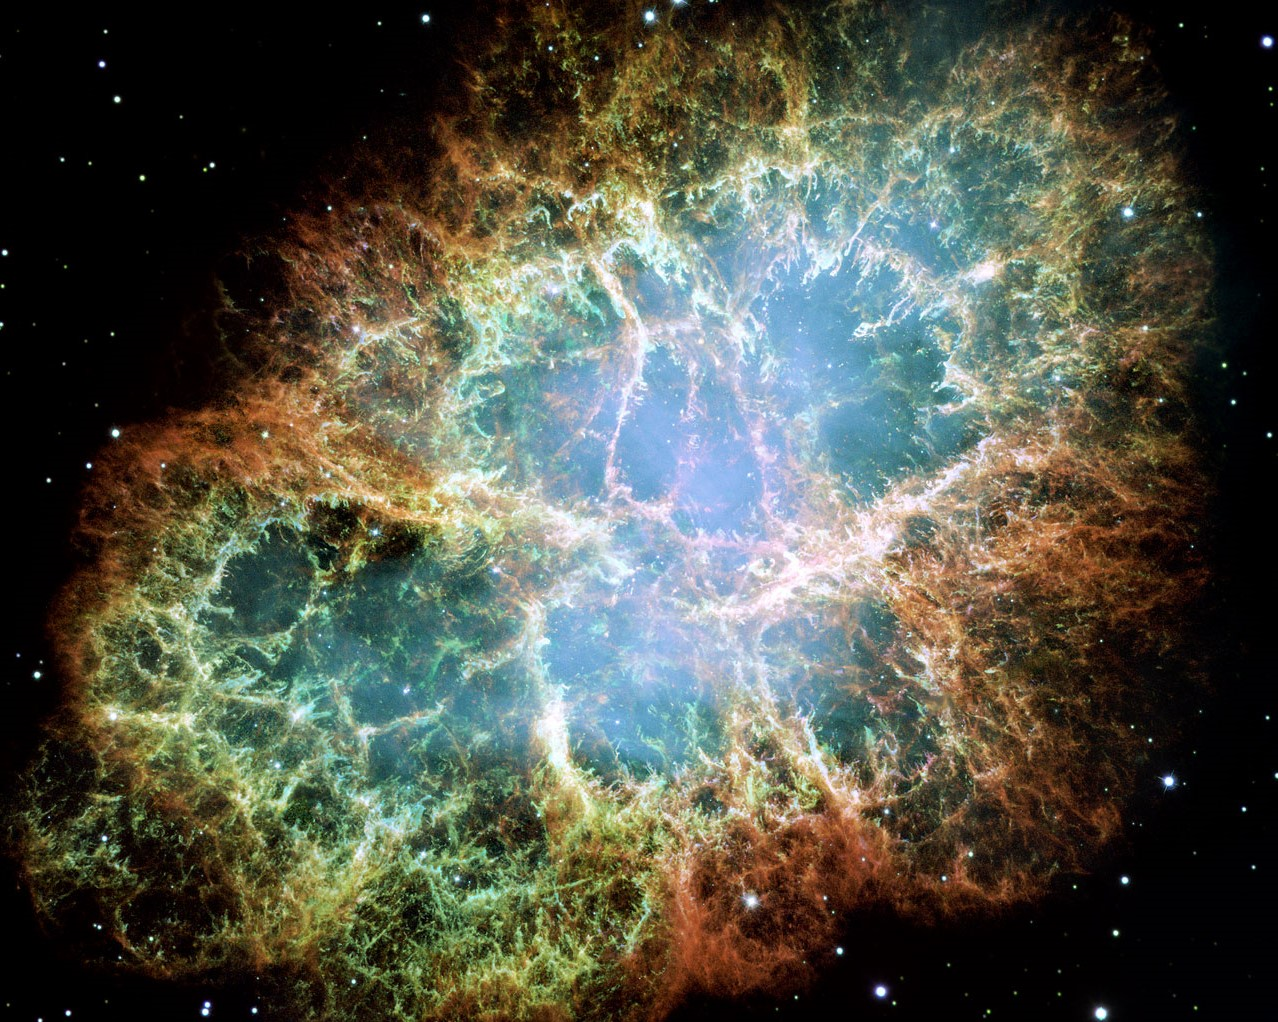
\includegraphics[width=\paperwidth, height =10cm]{../Crab.jpg}}
    \end{figure}
\end{titlepage}

%%%%%%%%%%%%%%%%%%%%%%%
\tableofcontents



%%%%%%%%%%%%%%%%%%%%%%%%%%%%%%%%%%%%% Part 1
\part{Thermodynamics}

%%%%%%%%%%%%%%%%%%%%%% Chapter 1.1
\chapter{Energy in Thermal Physics}

%%%%%%%%%%%%%%%%%%%% Section 1.1.1
\section{Basic Notation and Work}

\begin{defn}
    Thermodynamics is a \Emph{phenomenological} description of properties of \Emph{macroscopic systems} in \Emph{thermal equilibrium}.
\end{defn}

By a phenomenological description we mean a discription based on observations and direct experience of the experimenter with the system, considered as a ``black box" (a system whose internal structure is unknown, or is just not considered). The task of thermodynamics is to define appropriate physical quanitities, \Emph{state quantities}, which characterize macroscopic properties of matter, that is \Emph{macrostates}, in a way which is as unambiguous as possible, and to relate these quantities by means of universally valid equations.

\begin{defn}[Systems]
    There are a number of different thermodynamic systems. In particular we define a thermodynamic system, in general, to be an arbitrary amount of matter, the properties of which can be uniquely and completely described by specifying certain macroscopic parameters. We summarize them as follows: \begin{itemize}
        \item \Emph{Thermodynamic or Macroscopic System:} A system consisting of a large number of constituents. For example, a mole of gas (approximately $10^{23}$ particles) can be considered as a macroscopic system.
        \item \Emph{Isolated Thermodynamic System:} A system which exhibits no exchange of any type with the surroundings; no exchange of work, heat, matter, etc. The total energy (mechanical, electrical, etc.) is a conserved quantity for such a system, and can thus be used to characterize the macrostate.
        \item \Emph{Closed Theormodynamic System:} A system which exhibits no exchange of matter with its surroundings. Hence, energy exchange is allowed, so energy is no longer a conserved quantity and can fluctuate due to exchange with the surroundings. The termperature, particle number, and volume of the system can characterize the macrostate.
        \item \Emph{Open Thermodynamic System:} A system for which it is possible for exchange of any type with the surroundings (work, heat, matter, etc.). Energy and particle number are both not conserved. But, temperature and chemical potential can still be used to characterize a macrostate.
    \end{itemize}
\end{defn}

If the properties of a system are the same for any part of it, one calls such a system \Emph{homogeneous}. On the other hand, if the properties change discontinuously at certain marginal surfaces, the system is \Emph{heterogeneous}, with the homogeneous portions of the system called \Emph{phases} and the separating surfaces \Emph{phase boundaries}. 

\begin{defn}
    The macroscopic quantities which describe a system are called state quantities.
\end{defn}

\begin{eg}
    Examples of state quantities are the system's energy $E$, its volume $V$, its particle number $N$, its entropy $S$, its temperature $T$, the pressure $P$, the chemical potential $\mu$, the charge $q$, the dipole momentum, the refractive index, the viscosity, the chemical composition, and the size of phase boundaries.
\end{eg}

However, microscopic quantities do not fall under the umbrella of state quantities.

\begin{defn}[Equilibrium]
    Two thermodynamic systems are in \Emph{equilibrium} if and only if they are in contact such that they can exchange a given conserved quantity (for example particles) and they are relaxed to a state in which there is no average net transfer of that quantity between them anymore. A thermodynamic system $S$ is in equilibrium with itself, if and only if, all its subsystems are in equilibrium with each other. In this case, $S$ is called an \Emph{equilibrium} system.
\end{defn}

From this definition we find that different types of exchanged quanitities can lead to different types of equilibria: 

\begin{table}[H]
    \centering
    \begin{tabular}{c|c}
        \hline
        Exchanged Quantity & Type of Equilibrium \\ \hline \hline
        Particles/Matter & Diffusive Equilibrium \\ 
        Work & Mechanical Equilibrium \\
        Heat & Thermal Equilibrium \\ \hline
    \end{tabular}
\end{table}

\begin{defn}
    \Emph{Complete Thermodynamic Equilibrium} corresponds to a state where all the conserved fluxes between two coupled thermodynamic systems vanish.
\end{defn}

A way of testing if a given system is in a complete thermodynamic equilibrium is if the properties of the system do not change appreciably over the observation time, which is to say the properties reflect the true asymptotic long-term properties after any initial relaxation time is over.

The state of thermodynamic systems in complete thermodynamic equilibrium can be described by a set of independent \Emph{thermodynamic coordinates} or \Emph{state variables}; this fact is based on empirical observations. 

\subsection{Boyle-Mariotte's Experiment}

\begin{law}
    For a given mass of gas at a constant temperature $T$, the volume $V$ is inverseley proportional to the pressure $P$: $V \propto P^{-1}$.
\end{law}

We consider Robert Boyle's (1627-1691) experiment, conducted at room temperature, which should remain constant during the time of the experiment. We use a vertical tube with markings to indicate the volume of gas, and oil at the bottom. By applying pressure on the oil, we also exert a pressure on the air in the tube above the oil, causing the volume to decrease. Drawing the graph of volume versus $P^{-1}$ we obtain a straight line, so $V\cdot P = C$ for some constant $C$, given a fixed temperature. As further measurements show, the constant is proportional to the temperature $T$, so $V\cdot P \propto T$. More precisely, the full equation of a state of simple low-density gase is given by \begin{equation}
    \boxed{PV = Nk_BT}
\end{equation}
where $N$ is the number of gas particles and $k_B \approx 1.381\times 10^{-23}\;J/K$ is a natural constant called the \Emph{Boltzmann's constant}. The above equation is called the \Emph{ideal gas law} or the \Emph{equation of state for an ideal gas} since it relates the three state variables, or thermodynamic coordinates, $P$, $V$, and $T$ at equilibrium.

\subsubsection{Mechanical Derivation}

We now sketch a derivation of the ideal gas law using an atomistic theory governed by Newton's Laws. First assume there is a single molecule or atom bouncing around in a volume $V = AL$, where $L$ is the length along the $x$-direction and $A$ is the area of a side parallel to the $yz$-plane:

\begin{center}
    \begin{tikzpicture}[x=0.75pt,y=0.75pt,yscale=-1.4,xscale=1.4]
%uncomment if require: \path (0,398); %set diagram left start at 0, and has height of 398

%Shape: Cube [id:dp41058044355698486] 
\draw   (130,134) -- (154,110) -- (240,110) -- (240,166) -- (216,190) -- (130,190) -- cycle ; \draw   (240,110) -- (216,134) -- (130,134) ; \draw   (216,134) -- (216,190) ;
%Straight Lines [id:da3652266253176417] 
\draw    (132,200) -- (208,200) ;
\draw [shift={(210,200)}, rotate = 180] [color={rgb, 255:red, 0; green, 0; blue, 0 }  ][line width=0.75]    (6.56,-1.97) .. controls (4.17,-0.84) and (1.99,-0.18) .. (0,0) .. controls (1.99,0.18) and (4.17,0.84) .. (6.56,1.97)   ;
\draw [shift={(130,200)}, rotate = 0] [color={rgb, 255:red, 0; green, 0; blue, 0 }  ][line width=0.75]    (6.56,-1.97) .. controls (4.17,-0.84) and (1.99,-0.18) .. (0,0) .. controls (1.99,0.18) and (4.17,0.84) .. (6.56,1.97)   ;
%Straight Lines [id:da08447016298808463] 
\draw    (166.89,172.06) -- (190.59,155.21) ;
\draw [shift={(192.22,154.06)}, rotate = 504.61] [color={rgb, 255:red, 0; green, 0; blue, 0 }  ][line width=0.75]    (6.56,-1.97) .. controls (4.17,-0.84) and (1.99,-0.18) .. (0,0) .. controls (1.99,0.18) and (4.17,0.84) .. (6.56,1.97)   ;
%Curve Lines [id:da14521036207082538] 
\draw    (268.22,143.72) .. controls (250.49,160.14) and (256.69,125.13) .. (232.99,150.84) ;
\draw [shift={(231.89,152.06)}, rotate = 311.76] [color={rgb, 255:red, 0; green, 0; blue, 0 }  ][line width=0.75]    (6.56,-1.97) .. controls (4.17,-0.84) and (1.99,-0.18) .. (0,0) .. controls (1.99,0.18) and (4.17,0.84) .. (6.56,1.97)   ;
%Straight Lines [id:da5265921627377463] 
\draw  [dash pattern={on 0.84pt off 2.51pt}]  (130,190) -- (141.22,190) ;
\draw [shift={(143.22,190)}, rotate = 180] [color={rgb, 255:red, 0; green, 0; blue, 0 }  ][line width=0.75]    (4.37,-1.32) .. controls (2.78,-0.56) and (1.32,-0.12) .. (0,0) .. controls (1.32,0.12) and (2.78,0.56) .. (4.37,1.32)   ;
%Straight Lines [id:da8512625721822618] 
\draw  [dash pattern={on 0.84pt off 2.51pt}]  (130,190) -- (137.8,182.35) ;
\draw [shift={(139.22,180.94)}, rotate = 495.52] [color={rgb, 255:red, 0; green, 0; blue, 0 }  ][line width=0.75]    (4.37,-1.32) .. controls (2.78,-0.56) and (1.32,-0.12) .. (0,0) .. controls (1.32,0.12) and (2.78,0.56) .. (4.37,1.32)   ;
%Straight Lines [id:da2755149870872269] 
\draw  [dash pattern={on 0.84pt off 2.51pt}]  (130,190) -- (130,181.94) ;
\draw [shift={(130,179.94)}, rotate = 450] [color={rgb, 255:red, 0; green, 0; blue, 0 }  ][line width=0.75]    (4.37,-1.32) .. controls (2.78,-0.56) and (1.32,-0.12) .. (0,0) .. controls (1.32,0.12) and (2.78,0.56) .. (4.37,1.32)   ;

% Text Node
\draw (167,198) node [anchor=north west][inner sep=0.75pt]  [font=\scriptsize,color={rgb, 255:red, 255; green, 0; blue, 0 }  ,opacity=1 ]  {$L$};
% Text Node
\draw (166.89,172.06) node [anchor=center][inner sep=0.75pt]  [font=\LARGE,color={rgb, 255:red, 255; green, 0; blue, 0 }  ,opacity=1 ]  {$\cdot $};
% Text Node
\draw (170.56,151.96) node [anchor=north west][inner sep=0.75pt]  [font=\scriptsize,color={rgb, 255:red, 255; green, 0; blue, 0 }  ,opacity=1 ]  {$\vec{v}$};
% Text Node
\draw (269.56,135.96) node [anchor=north west][inner sep=0.75pt]  [font=\scriptsize,color={rgb, 255:red, 255; green, 0; blue, 0 }  ,opacity=1 ]  {$A$};
% Text Node
\draw (142.56,189.84) node [anchor=north west][inner sep=0.75pt]  [font=\tiny]  {$x$};
% Text Node
\draw (140.89,176.51) node [anchor=north west][inner sep=0.75pt]  [font=\tiny]  {$y$};
% Text Node
\draw (124.89,173.84) node [anchor=north west][inner sep=0.75pt]  [font=\tiny]  {$z$};


\end{tikzpicture}
\end{center}

After many perfectly ellastic collisions against the wall, the average pressure directly on the wall is \begin{equation*}
    \overline{p} = \frac{\overline{F}_{x,on\;wall}}{A} = -\frac{\overline{F}_{x,on\;molecule}}{A} = -\frac{m\overline{\frac{\Delta v_x}{\Delta t}}}{A} 
\end{equation*}
The time it takes for a full round trip is $\Delta t = 2L/v_x$. When it undergoes one elastic collision, its change in velocity is $\Delta v_x = -2v_x$. Together these give \begin{equation*}
    \overline{p} = -\frac{m(-2v_x/(2L/v_x))}{A} = \frac{mv_x^2}{LA} = \frac{mv_x^2}{V}
\end{equation*}
Now, if we extend to $N >> 1$ non-interacting molecules, each colliding with the walls totally elastically, then we can forgoe the averageness of the pressure to obtain \begin{equation*}
    pV = m\sum_{i=1}^N(v_x^2)_i = mN\overline{v_x^2} = Nk_BT
\end{equation*}
using the ideal gas law at the end, which gives the relation \begin{equation*}
    \overline{K}_x = \overline{\frac{1}{2}mv_x^2} = \frac{1}{2}k_BT
\end{equation*}
Then we find that the total mean kinetic energy is \begin{equation}
    \overline{K} = \frac{1}{2}m\overline{v_x^2}+\frac{1}{2}m\overline{v_y^2}+\frac{1}{2}m\overline{v_z^2} = \frac{3}{2}k_BT
\end{equation}

\begin{defn}
    The \Emph{Root-mean square speed} of each atom/molecule is defined as \begin{equation*}
        v_{RMS} = \sqrt{\overline{v^2}}
    \end{equation*}
\end{defn}

In general the RMS speed is often a close approximation of the average speed. In this case we have $v_{RMS} = \sqrt{3k_BT/m}$.


\subsection{Work}

\begin{defn}
    Given a vector force field $\vec{F}$ defined along a path $\gamma$, the \Emph{work} $W$ is of $\vec{F}$ along $\gamma$ is defined to be: \begin{equation}
        W = \int_{\gamma}\vec{F}\cdot d\vec{r}
    \end{equation}
\end{defn}

\begin{rec}
    Recall that pressure is force per unit area, so we have that \begin{equation*}
        P = \frac{F}{A}
    \end{equation*}
    where $F$ is the normal component of the force to the area $A$. More precisely, pressure is the proportionality constant that relates the force and normal vectors: \begin{equation*}
        d\vec{F}_n = -pd\vec{A}
    \end{equation*}
    where $\vec{F}_n$ denotes the normal component of the force vector $\vec{F}$.
\end{rec}


\begin{eg}
    Consider the compression of a gas by a piston with a constant force of magnitude $F$.
    \begin{center}
    \begin{tikzpicture}[x=0.75pt,y=0.75pt,yscale=-1.2,xscale=1.2]
%uncomment if require: \path (0,398); %set diagram left start at 0, and has height of 398

%Shape: Rectangle [id:dp9125760638904235] 
\draw   (100,110) -- (200,110) -- (200,160) -- (100,160) -- cycle ;
%Straight Lines [id:da19743423815417427] 
\draw    (200,110) -- (230,110) ;
%Straight Lines [id:da17599416360044806] 
\draw    (200,160) -- (230,160) ;
%Straight Lines [id:da37025754978607806] 
\draw [color={rgb, 255:red, 255; green, 27; blue, 0 }  ,draw opacity=1 ]   (200,110) -- (200,160) ;
%Straight Lines [id:da5752016333947421] 
\draw [color={rgb, 255:red, 255; green, 27; blue, 0 }  ,draw opacity=1 ]   (200,135) -- (250,135) ;
%Straight Lines [id:da4588247522685671] 
\draw    (230,127) -- (222,127) ;
\draw [shift={(220,127)}, rotate = 360] [color={rgb, 255:red, 0; green, 0; blue, 0 }  ][line width=0.75]    (4.37,-1.32) .. controls (2.78,-0.56) and (1.32,-0.12) .. (0,0) .. controls (1.32,0.12) and (2.78,0.56) .. (4.37,1.32)   ;
%Curve Lines [id:da22459360243367987] 
\draw [line width=0.75]    (281.89,123.39) .. controls (280.27,107.22) and (224.4,110.81) .. (204.92,121.69) ;
\draw [shift={(203.22,122.72)}, rotate = 326.56] [color={rgb, 255:red, 0; green, 0; blue, 0 }  ][line width=0.75]    (6.56,-1.97) .. controls (4.17,-0.84) and (1.99,-0.18) .. (0,0) .. controls (1.99,0.18) and (4.17,0.84) .. (6.56,1.97)   ;
%Straight Lines [id:da04861500853364609] 
\draw    (200,170) -- (192,170) ;
\draw [shift={(190,170)}, rotate = 360] [color={rgb, 255:red, 0; green, 0; blue, 0 }  ][line width=0.75]    (4.37,-1.32) .. controls (2.78,-0.56) and (1.32,-0.12) .. (0,0) .. controls (1.32,0.12) and (2.78,0.56) .. (4.37,1.32)   ;
%Straight Lines [id:da2692578781738837] 
\draw    (200,167) -- (200,173) ;

% Text Node
\draw (231,122.4) node [anchor=north west][inner sep=0.75pt]  [font=\tiny,color={rgb, 255:red, 246; green, 12; blue, 12 }  ,opacity=1 ]  {$\vec{F}$};
% Text Node
\draw (237,125) node [anchor=north west][inner sep=0.75pt]  [font=\tiny] [align=left] {(const.)};
% Text Node
\draw (270.89,125.89) node [anchor=north west][inner sep=0.75pt]  [font=\tiny] [align=left] {Piston area:};
% Text Node
\draw (311.89,125.4) node [anchor=north west][inner sep=0.75pt]  [font=\tiny,color={rgb, 255:red, 255; green, 0; blue, 0 }  ,opacity=1 ]  {$\mathcal{A}$};
% Text Node
\draw (108.56,114.4) node [anchor=north west][inner sep=0.75pt]  [font=\small]  {$\cdot $};
% Text Node
\draw (128.56,134.4) node [anchor=north west][inner sep=0.75pt]  [font=\small]  {$\cdot $};
% Text Node
\draw (128.56,134.4) node [anchor=north west][inner sep=0.75pt]  [font=\small]  {$\cdot $};
% Text Node
\draw (139.89,121.07) node [anchor=north west][inner sep=0.75pt]  [font=\small]  {$\cdot $};
% Text Node
\draw (159.89,141.07) node [anchor=north west][inner sep=0.75pt]  [font=\small]  {$\cdot $};
% Text Node
\draw (127.56,112.07) node [anchor=north west][inner sep=0.75pt]  [font=\small]  {$\cdot $};
% Text Node
\draw (161.56,117.4) node [anchor=north west][inner sep=0.75pt]  [font=\small]  {$\cdot $};
% Text Node
\draw (181.56,137.4) node [anchor=north west][inner sep=0.75pt]  [font=\small]  {$\cdot $};
% Text Node
\draw (110.22,132.4) node [anchor=north west][inner sep=0.75pt]  [font=\small]  {$\cdot $};
% Text Node
\draw (179.22,114.73) node [anchor=north west][inner sep=0.75pt]  [font=\small]  {$\cdot $};
% Text Node
\draw (142.89,141.4) node [anchor=north west][inner sep=0.75pt]  [font=\small]  {$\cdot $};
% Text Node
\draw (168.22,127.73) node [anchor=north west][inner sep=0.75pt]  [font=\small]  {$\cdot $};
% Text Node
\draw (148.22,112.73) node [anchor=north west][inner sep=0.75pt]  [font=\small]  {$\cdot $};
% Text Node
\draw (123.56,124.07) node [anchor=north west][inner sep=0.75pt]  [font=\small]  {$\cdot $};
% Text Node
\draw (111.56,142.73) node [anchor=north west][inner sep=0.75pt]  [font=\small]  {$\cdot $};
% Text Node
\draw (192,173.4) node [anchor=north west][inner sep=0.75pt]  [font=\tiny]  {$\Delta x$};


\end{tikzpicture}
\end{center}
    so the work is \begin{equation*}
        W = \int_{\gamma}\vec{F}\cdot d\vec{r} = F\int_{\gamma}dr = F\Delta x = PA\Delta x = -P\Delta V
    \end{equation*}
    where $P$ is the pressure and $\Delta V$ is the change in volume. Since the change in volume is negative, the work $W$ done on the system (here the gas) is positive: Energy is added to the system by a force (macroscopic) process (here the piston). $W< 0$ if energy is removed from the system.
\end{eg}


\begin{defn}
    The generalized differential form for work is given by \begin{equation}
        \delta W = \sum_{i=1}^mJ_idq_i
    \end{equation}
    where $q_i$ are the generalized coordinates and the $J_i$ are the conjugate generalized forces such that $J_idq_i$ has units of energy. This is possible when the system is undergoing an infinitesimal quasi-static transformation.
\end{defn}

Here are a few examples of generalized coordinates and their corresponding generalized conjugate forces:

\begin{table}[H]
    \centering
    \begin{tabular}{c|c|c}
        \hline
        & Generalized Force $J_i$ & Generalized Coordinate $dq_i$ \\ \hline \hline
        Pressure & $-P$ & $dV$ (change in volume) \\ 
        Surface tension & $\sigma$ & $dS$ (change in surface area) \\
        Magnetic field & $\vec{B}_0$ & $d\vec{m}$ (change in magnetic moment) \\
        Electric field & $\vec{E}$ & $d\vec{P}$ (change in electric dipole moment) \\\hline
    \end{tabular}
\end{table}

\begin{defn}
    Differential changes in a systems property are said to be \Emph{quasi-static} if the changes occur on time scales much longer than the relaxation time such that the system remains in equilibrium at all times.
\end{defn}

To ensure thermodynamics is a self-consistent description of macroscopic systems in thermal equilibrium we must assume that the differential changes $\delta W$ are quasi-static. This also ensures that we can describe the state of such a thermodynamic system by a set of thermodynamic coordinates at all times, which is to state at any stage of the process the thermodynamic coordinates of the system exist and can in principle be computed. 

Depending on the macroscopic generalized force, the work necessary to transfer a thermodynamic system in complete thermodynamic equilibrium from state $A$ to state $B$ might or might not depend on the path taken. For example, if $\gamma_1$ and $\gamma_2$ are two paths from state $A$ to state $B$, it is possible that $\int_{\gamma_1}\delta W \neq \int_{\gamma_2}\delta W$. (Note that this justifies the use of the notation $\delta W$ over $dW$, which would denote an exact differential)


\begin{defn}
    State quantities which are proportional to the amount of matter in a system are called \Emph{extensive}, and are consequently additive when looking at subsystems.
\end{defn}

\begin{defn}
    State quantities which are independent of the amount of matter in the system are called \Emph{intensive}, and are not additive for the particular phases of the system.
\end{defn}

Intensive quantities are indicators of equilibrium. 


\subsection{Conservative Forces}

\begin{rec}
    Recall that a conservative force is a force $\vec{F}$ with an associated potential energy function $E$ such that $\vec{F} = \nabla E$.
\end{rec}

\begin{prop}
    If the macroscopic generalized force $\vec{J}$, depending on $m$ generalized coordinates $q_i$, is conservative with potential energy $E_{pot}$ which is twice continuously differentiable and the domain of integration is simply connected, then the following are equivalent:
    \begin{itemize}
        \item $\vec{J}(\vec{q}) = -\nabla E_{pot}(\vec{q})$
        \item $dW$ is an exact differential form, so $$\int_{\gamma}dW = \int_{\gamma}\vec{J}\cdot d\vec{r}$$ depends only on the endpoints of $\gamma$.
        \item For any simple closed path $\gamma$, $$\oint_{\gamma}dW = \oint_{\gamma}\vec{J}\cdot d\vec{r} = 0$$
        \item The curl of $\vec{J}$ is trivial over the domain of integration $$\nabla \times \vec{J} = 0$$ provided that $m = 3$
        \item For all $i,j \in \{1,2,...,m\}$, we have that \begin{equation*}
                \frac{\partial J_i}{\partial q_j} - \frac{\partial J_j}{\partial q_i} = 0
        \end{equation*}
        \item The differential $dW$ is exact, and we have that \begin{equation*}
                dW = -\nabla E_{pot}\cdot d\vec{r} = -\sum_{i=1}^m\frac{\partial E_{pot}}{\partial q_i}dq_i = -dE_{pot}
        \end{equation*}
    \end{itemize}
\end{prop}


\begin{defn}
    For a function $A(q_1,q_2,...,q_m)$ the \Emph{total differential} or \Emph{exact differential} of $A$ is given by \begin{equation*}
        dA = \sum_{i=1}^m\frac{\partial A}{\partial q_i}dq_i
    \end{equation*}
    This corresponds to a generalized chain rule: \begin{equation*}
        \frac{dA}{dt} = \nabla A\cdot \frac{d}{dt}\vec{q} = \sum_{i=1}^m\frac{\partial A}{\partial q_i}\frac{dq_i}{dt}
    \end{equation*}
    called the \Emph{total derivative} of $A$ with respect to $t$. An exact differential corresponds to an \Emph{integrable differential form}: \begin{equation*}
        \int_{\gamma}\sum_{i=1}^m\frac{\partial A}{\partial q_i}dq_i = \int_{\gamma}dA = A(\vec{q}_f) - A(\vec{q}_i)
    \end{equation*}
    where $\vec{q}_i$ and $\vec{q}_f$ are the initial and final point of the path $\gamma$, respectively.
\end{defn}

Consequently, an integrable, or exact, differential form does not depend on the path taken and in physics we would consider $A$ to be a potential function. 

\begin{note}
    For non-conservative forces, $\delta W$ is an \Emph{inexact differential form}.
\end{note}

\begin{thm}
    A differential form $$\delta A \equiv \sum_{i=1}^ma_i(q_1,q_2,...,q_m)dq_i$$ for functions $a_i:D \subseteq \R^m\rightarrow \R$ is exact if and only if \begin{equation*}
        \frac{\partial a_i}{\partial q_j} = \frac{\partial a_j}{\partial q_i}
    \end{equation*}
    for all $i,j \in \{1,2,...,m\}$.
\end{thm}

\begin{defn}
    An \Emph{integrating factor} $\mu$ is a factor that makes an inexact differential form exact upon multiplication.
\end{defn}

\begin{thm}
    For $m = 2$, an integrating factor always exists. Specifically, for $\delta A = a_1dx_1+a_2dx_2$, we can define $df:= \mu \delta A = (\mu a_1)dx_1 + (\mu a_2)dx_2$, with $\mu$ determined non-uniquely by the equation \begin{equation*}
        \frac{\partial (\mu a_1)}{\partial x_2} = \frac{\partial (\mu a_2)}{\partial x_1}
    \end{equation*}
\end{thm}


%%%%%%%%%%%%%%%%%%%% Section 1.1.2
\section{Equipartition Theorem}

\begin{namthm}[Equipartition Theorem]
    Every degree of freedom of a system in thermodynamic equilibrium, which appear only quadratically in the total energy, constributes an average energy of $\frac{1}{2}Nk_BT$ to the total energy of the system.
\end{namthm}

First, what exactly is a `degree of freedom'? In colloquil terms, a degree of freedom tells you about what the atom or molecule can actually do - maybe it can move around (translate), or vibrate, or rotate, or produce sound, or emit light, or a host of other things. Each of these capabilities contributes an energy of $\frac{1}{2}k_BT$ to the system's energy. 

Now, recall that the kinetic energy of a rotating body given a diagonalized inertial basis $I_{ii}$, is \begin{equation}
    K_{rot} = \frac{1}{2}(I_{xx}w_x^2+I_{yy}w_y^2+I_{zz}w_z^2)
\end{equation}
and $w_i$ are the angular frequences associated with the angular velocity of the body in this basis. Each of these terms is quadratic, so each one corresponds to a degree of freedom. 

We can conclude that the total energy of the system in some limit is \begin{equation*}
    \frac{f}{2}Nk_BT
\end{equation*}
where $f$ is the number of degrees of freedom.

%%%%%%%%%%%%%%%%%%%% Section 1.1.3
\section{Heat and the 1st Law of Thermodynamics}

\begin{defn}
    Recall that work corresponds to the change in energy of a thermodynamic system by a \Emph{macroscopically forced process}. On the other hand the \Emph{heat} $Q$ is the energy added to or removed from a thermodynamic system by a \Emph{spontaneous process} (that is not forced).
\end{defn}

Heat can be also stated as the amount of energy that spontaneously flows between two systems: heat moves from the system at higher temperature to the system at lower temperature (2nd law of thermodynamics to be covered later). Note we can define the temperature through the equipartition theorem as a measure of the total energy of the system $E$: $T \approx 2E/fk_B$, where $f$ is the number of degrees of freedom.

We note that negative $Q$ implies removing energy while positive $Q$ implies adding energy.

For example, consider the energy transfer between a cooking plate and a pot of water. The origin of this type of process lies in the underlying microscopic dynamics, which we will explore using Statistical Mechanics. 

\begin{law}[First Law of Thermodynamics]
    For an isolated thermodynamic system, the total \Emph{internal energy} $U$ is a constant and $dU = 0$. By the definition of internal energy, $dU$ is an exact differential; consequently, $U$ should be unique for a given state. For various systems we have the following: \begin{itemize}
        \item For a closed system, $dU = \delta Q + \delta W$. 
        \item For an open system, $dU = \delta Q + \delta W + \delta E_c$, with $$\delta E_c := \sum_{i=1}^{\alpha}\mu_idN_i$$ where $N_i$ is the number of particles of type $i$ and $\mu_i$ is the \Emph{chemical potential} associated with particles of type $i$ for all $1 \leq i \leq \alpha$ with $\alpha$ being the number of different particle types. The chemical potential corresponds to the energy needed to add a particle of type $i$ to a given thermodynamic system while no other type of energy is exchanged, which is to say $\delta W = 0$ and $\delta Q = 0$.
    \end{itemize}
\end{law}

In summary, the empirical first law is a reformulation of the conservation of energy and requires the inclusion of heat. 





%%%%%%%%%%%%%%%%%%%%%% Chapter 1.2
\chapter{Thermodynamical Systems}


%%%%%%%%%%%%%%%%%%%% Section 1.2.1
\section{The 0th Law of Thermodynamics}

We now wish to define the concept of temperature from a \Emph{macroscopic} perspective, to ensure our theoretical framework of thermodynamics is a self-consistent description of macroscopic systems in thermal equilibrium. The empirical principal we proceed with in our construction is that two systems which are in thermal equilibrium with one another should share the same ``temperature." Before we showed a derivation of the temperature in terms of kinetic energy from a microscopic perspective of sparse (non-dense) gas - this belongs to the area of Statistical mechanics.

Now, the $0$th law of thermodynamics describes the transitivity of the equilibrium relation for systems:

\begin{law}[0th Law of Thermodynamics]
    If two systems, $A$ and $B$, are separately in equilibrium with a third system, $C$, then they are also in thermal equilibrium with one another.
\end{law}

Indeed we can depict this as follows:

\begin{center}
\begin{tikzpicture}[x=0.75pt,y=0.75pt,yscale=-1,xscale=1]
%uncomment if require: \path (0,398); %set diagram left start at 0, and has height of 398

%Shape: Rectangle [id:dp7440238011885612] 
\draw   (100,120) -- (200,120) -- (200,173.5) -- (100,173.5) -- cycle ;
%Shape: Rectangle [id:dp00894291260356117] 
\draw   (242,120) -- (342,120) -- (342,173.5) -- (242,173.5) -- cycle ;
%Shape: Rectangle [id:dp3516092606802361] 
\draw   (100,210) -- (342,210) -- (342,282.5) -- (100,282.5) -- cycle ;
%Straight Lines [id:da2634357285779194] 
\draw    (292,175.08) -- (292,208) ;
\draw [shift={(292,210)}, rotate = 270] [color={rgb, 255:red, 0; green, 0; blue, 0 }  ][line width=0.75]    (10.93,-3.29) .. controls (6.95,-1.4) and (3.31,-0.3) .. (0,0) .. controls (3.31,0.3) and (6.95,1.4) .. (10.93,3.29)   ;
\draw [shift={(292,173.08)}, rotate = 90] [color={rgb, 255:red, 0; green, 0; blue, 0 }  ][line width=0.75]    (10.93,-3.29) .. controls (6.95,-1.4) and (3.31,-0.3) .. (0,0) .. controls (3.31,0.3) and (6.95,1.4) .. (10.93,3.29)   ;
%Straight Lines [id:da874447176315235] 
\draw    (525.67,146.8) -- (563.67,146.8) ;
\draw [shift={(565.67,146.8)}, rotate = 180] [color={rgb, 255:red, 0; green, 0; blue, 0 }  ][line width=0.75]    (10.93,-3.29) .. controls (6.95,-1.4) and (3.31,-0.3) .. (0,0) .. controls (3.31,0.3) and (6.95,1.4) .. (10.93,3.29)   ;
\draw [shift={(523.67,146.8)}, rotate = 0] [color={rgb, 255:red, 0; green, 0; blue, 0 }  ][line width=0.75]    (10.93,-3.29) .. controls (6.95,-1.4) and (3.31,-0.3) .. (0,0) .. controls (3.31,0.3) and (6.95,1.4) .. (10.93,3.29)   ;
%Straight Lines [id:da5304557286713043] 
\draw    (150,175.08) -- (150,208) ;
\draw [shift={(150,210)}, rotate = 270] [color={rgb, 255:red, 0; green, 0; blue, 0 }  ][line width=0.75]    (10.93,-3.29) .. controls (6.95,-1.4) and (3.31,-0.3) .. (0,0) .. controls (3.31,0.3) and (6.95,1.4) .. (10.93,3.29)   ;
\draw [shift={(150,173.08)}, rotate = 90] [color={rgb, 255:red, 0; green, 0; blue, 0 }  ][line width=0.75]    (10.93,-3.29) .. controls (6.95,-1.4) and (3.31,-0.3) .. (0,0) .. controls (3.31,0.3) and (6.95,1.4) .. (10.93,3.29)   ;
%Straight Lines [id:da12969934099335645] 
\draw    (359.4,198.5) -- (404.18,198.5)(359.4,201.5) -- (404.18,201.5) ;
\draw [shift={(412.18,200)}, rotate = 180] [color={rgb, 255:red, 0; green, 0; blue, 0 }  ][line width=0.75]    (10.93,-3.29) .. controls (6.95,-1.4) and (3.31,-0.3) .. (0,0) .. controls (3.31,0.3) and (6.95,1.4) .. (10.93,3.29)   ;
\draw [shift={(351.4,200)}, rotate = 0] [color={rgb, 255:red, 0; green, 0; blue, 0 }  ][line width=0.75]    (10.93,-3.29) .. controls (6.95,-1.4) and (3.31,-0.3) .. (0,0) .. controls (3.31,0.3) and (6.95,1.4) .. (10.93,3.29)   ;
%Shape: Rectangle [id:dp038213352648847954] 
\draw   (423,120) -- (523,120) -- (523,173.5) -- (423,173.5) -- cycle ;
%Shape: Rectangle [id:dp8987344627936489] 
\draw   (565,120) -- (665,120) -- (665,173.5) -- (565,173.5) -- cycle ;
%Shape: Rectangle [id:dp787394422240979] 
\draw   (423,210) -- (665,210) -- (665,282.5) -- (423,282.5) -- cycle ;
%Straight Lines [id:da9453296500738602] 
\draw    (615,175.08) -- (615,208) ;
\draw [shift={(615,210)}, rotate = 270] [color={rgb, 255:red, 0; green, 0; blue, 0 }  ][line width=0.75]    (10.93,-3.29) .. controls (6.95,-1.4) and (3.31,-0.3) .. (0,0) .. controls (3.31,0.3) and (6.95,1.4) .. (10.93,3.29)   ;
\draw [shift={(615,173.08)}, rotate = 90] [color={rgb, 255:red, 0; green, 0; blue, 0 }  ][line width=0.75]    (10.93,-3.29) .. controls (6.95,-1.4) and (3.31,-0.3) .. (0,0) .. controls (3.31,0.3) and (6.95,1.4) .. (10.93,3.29)   ;
%Straight Lines [id:da5113397508185176] 
\draw    (473,175.08) -- (473,208) ;
\draw [shift={(473,210)}, rotate = 270] [color={rgb, 255:red, 0; green, 0; blue, 0 }  ][line width=0.75]    (10.93,-3.29) .. controls (6.95,-1.4) and (3.31,-0.3) .. (0,0) .. controls (3.31,0.3) and (6.95,1.4) .. (10.93,3.29)   ;
\draw [shift={(473,173.08)}, rotate = 90] [color={rgb, 255:red, 0; green, 0; blue, 0 }  ][line width=0.75]    (10.93,-3.29) .. controls (6.95,-1.4) and (3.31,-0.3) .. (0,0) .. controls (3.31,0.3) and (6.95,1.4) .. (10.93,3.29)   ;

% Text Node
\draw (109.78,130.07) node [anchor=north west][inner sep=0.75pt]  [color={rgb, 255:red, 255; green, 0; blue, 0 }  ,opacity=1 ]  {$A$};
% Text Node
\draw (252.44,123.4) node [anchor=north west][inner sep=0.75pt]  [color={rgb, 255:red, 255; green, 0; blue, 0 }  ,opacity=1 ]  {$B$};
% Text Node
\draw (208.44,229.4) node [anchor=north west][inner sep=0.75pt]  [color={rgb, 255:red, 255; green, 0; blue, 0 }  ,opacity=1 ]  {$C$};
% Text Node
\draw (432.78,130.07) node [anchor=north west][inner sep=0.75pt]  [color={rgb, 255:red, 255; green, 0; blue, 0 }  ,opacity=1 ]  {$A$};
% Text Node
\draw (575.44,123.4) node [anchor=north west][inner sep=0.75pt]  [color={rgb, 255:red, 255; green, 0; blue, 0 }  ,opacity=1 ]  {$B$};
% Text Node
\draw (531.44,229.4) node [anchor=north west][inner sep=0.75pt]  [color={rgb, 255:red, 255; green, 0; blue, 0 }  ,opacity=1 ]  {$C$};
% Text Node
\draw (128.67,184.22) node [anchor=north west][inner sep=0.75pt]  [font=\scriptsize] [align=left] {{\fontfamily{ptm}\selectfont heat}};
% Text Node
\draw (296.67,186.22) node [anchor=north west][inner sep=0.75pt]  [font=\scriptsize] [align=left] {{\fontfamily{ptm}\selectfont heat}};
% Text Node
\draw (451.33,186.22) node [anchor=north west][inner sep=0.75pt]  [font=\scriptsize] [align=left] {{\fontfamily{ptm}\selectfont heat}};
% Text Node
\draw (534.67,132.89) node [anchor=north west][inner sep=0.75pt]  [font=\scriptsize] [align=left] {{\fontfamily{ptm}\selectfont heat}};
% Text Node
\draw (620,185.56) node [anchor=north west][inner sep=0.75pt]  [font=\scriptsize] [align=left] {{\fontfamily{ptm}\selectfont heat}};


\end{tikzpicture}
\end{center}

where the double-sided arrows labeled ``heat" correspond to equilibrium between the systems. This law leads to existence of the state function $\Theta$, known as the \Emph{empirical temperature}, such that systems in equilibrium are at the same temperature:

\begin{cor}
    The $0$th law of thermodynamics (transitivity of equilibria) implies the existence of temperature (state function).
\end{cor}
\begin{proof}
    Assume that systems $A$ and $C$ are allowed to exchange heat and that they are in thermal equilibrium with each other. The state of system $A$ is described by thermodynamic coordinates $A_1,A_2,...$ and that of $C$ by $C_1,C_2,...$. If now, for example, $A_1$ is changed, then this will potentially lead to changes in $A_2,A_3,...$ and $C_1,C_2,...$. Mathematically, this means that a function $f_{AC}$ exists such that \begin{equation*}
        f_{AC}(A_1,A_2,...,C_1,C_2,...) = 0,
    \end{equation*}
    which is to say the function is constant for all thermodynamic coordinates that correspond to a thermal equilibrium between $A$ and $C$. This has the form of a \Emph{constraint}. Similarly, we have another function $f_{BC}$ with \begin{equation*}
        f_{BC}(B_1,B_2,...,C_1,C_2,...) = 0,
    \end{equation*}
    describing the thermal equilibrium between systems $B$ and $C$, where the state coordinates of $B$ are $B_1,B_2,...$. For such physical constraints, the implicit function theorem applies and we can solve the above equations for any specific parameter, for example \begin{equation*}
        C_1 = F_{AC}(A_1,A_2,...,C_2,C_3,...)
    \end{equation*}
    and \begin{equation*}
        C_1 = F_{BC}(B_1,B_2,...,C_2,C_3,...)
    \end{equation*}
    for thermodynamic coordinates $A_1,A_2,...,B_1,B_2,...,C_2,C_3,...$ such that the constraints hold, so the systems are in thermodynamic equilibrium. Thus, as $C$ is separately in equilibrium with $A$ and $B$, this implies that \begin{equation*}
        F_{AC}(A_1,A_2,...,C_2,...) = F_{BC}(B_1,B_2,...,C_2,...)
    \end{equation*}
    Now the $0$th law ensures that $A$ and $B$ are also in thermal equilibrium so there is a function $f_{AB}$ such that \begin{equation*}
        f_{AB}(A_1,A_2,...,B_1,B_2,...) = 0
    \end{equation*}
    is the constraint describing the equilibrium. For any set of state parameters satisfying this equation, when substituting into $F_{AC} = F_{BC}$ the equality must hold quite independently of the state variables for $C$. Moving along the level surface described by this constraint, $F_{AC} = F_{BC}$ will remain valid irrespective of the state of $C$. This implies that we can cancel the $C_2,C_3,...$ state variables in the equation $F_{AC} = F_{BC}$ on the manifold described by $f_{AB} = 0$. Hence, we have after cancelling the $C_2,C_3,...$'s out of the equation, \begin{equation*}
        \Theta_A(A_1,A_2,...) = \Theta_B(B_1,B_2,...)
    \end{equation*}
    and this characterizes the equilibrium previously characterized by $f_{AB} = 0$. Thus, we have the existence of a universal property of systems in thermal equilibrium, namely the existence of a state function $\Theta$ that takes on identical values if systems are in thermal equilibrium, and this function specifies the \Emph{equation of state}. Hence, it fulfils the basic property of what one would naturally consider a temperature. We define $\Theta$ as the \Emph{empirical temperature}, which is scalar and not unique - we have many possible choices for $\Theta$ at his point. For a given fixed temperature $\Theta$, all allowed thermodynamic states of a system, say $A$, can be obtained by $\Theta_A(A_1,A_2,...) = \Theta$. These states are called the \Emph{isotherms}.
\end{proof}

We note that due to this, the zeroth law constrains the form of the constraint equation describing the equilibrium between two bodies such that it can be organized into an equality of two empirical temperature functions. 

\begin{rmk}
    \Emph{Isotherms} can be considered as manifolds, or level-surfaces, of the empirical temperature function in the space of state variables for a system.
\end{rmk}

\begin{defn}
    A \Emph{thermometer} is a system with some convenient macroscopic property that changes in a simple way as the equilibriumm macrostate changes.
\end{defn}


%%%%%%%%%%%%%%%%%%%% Section 1.2.2
\section{Heat Capacities}

We move to the question of how much heat (energy added through a spontaneous not-forced process) is needed to raise the temperature of a system by a given amount. Heat is often an inexact differential, $\delta Q$, (which is to say it is not-path independent), and hence not a function of the state variables (i.e. not a \Emph{state function}). Consequently, one needs to specify the path by which heat is supplied:

\begin{defn}
    The \Emph{heat capacities} are defined as $C_{\vec{X}} = \left(\frac{\partial Q}{dt}\right)_{\vec{X}}$, where $\vec{X}$ is the set of thermodynamic coordinates which are held constant during the heat supply $\delta Q$. The \Emph{specific heats} are defined as $c_{\vec{X}} = \left(\frac{\delta Q}{MdT}\right)_{\vec{X}}$ where $M$ is the mass of the system.
\end{defn}

Consequently, the heat capacity of a system is how much heat energy is needed to raise its temperature by one degree. The specific heat is the heat capacity per unit mass. 


\begin{eg}
    Examples of common specific heats are as follows: \begin{itemize}
        \item Water: $c_P \approx 4180\;J/(kg\;K)$ and $c_V \approx c_P$ at $T = 25^{\circ}C$, $p = 100\;kPa$, and $N$ fixed.
        \item Air: $c_P \approx 1010\; J/(kg\;K)$ and $c_V \approx 720\;J/(kg\;K)$ at $T = 25^{\circ}C$, $p = 100\;kPa$, and $N$ fixed.
    \end{itemize}
\end{eg}

\subsection{Closed Systems (Heat Capacities)}

Assume that the internal energy of a system is given by $U = U(T,q_1,...,q_m)$, which is to say the state of the system can be uniquely determined by the temperature and $\vec{q}$. Starting from the 1st law we have that \begin{equation*}
    \delta Q = dU - \delta W = dU - \sum_{i=1}^mJ_idq_i = \frac{\partial U}{\partial T}dT + \sum_{i=1}^m\left[\frac{\partial U}{\partial q_i} - J_i\right]dq_i
\end{equation*}
We consider as a first special case the absence of any external work, so $\delta W = 0$ and equivalently $\vec{q}$ is constant (for example, the volume for a gas being constant), so we have that \begin{equation*}
    C_{\vec{q}} = \left(\frac{\delta Q}{dT}\right)_{\vec{q}} = \left(\frac{\partial U}{\partial T}\right)_{\vec{q}}
\end{equation*}
As a second special case let us consider when all macroscopic generalized forces are constant, so $\vec{J}$ is constant (for example, the pressure for a gas is constant). We use the state functions $J_i=J_i(q_1,...,q_m,T)$, for $1 \leq i \leq m$, and we invert them to obtain $q_i = q_i(J_1,...,J_m,T)$ for $1 \leq i \leq m$ and make a change of variables: \begin{equation*}
    dq_i = \sum_{j=1}^m\frac{\partial q_i}{\partial J_j}dJ_j + \frac{\partial q_i}{\partial T}dT = \frac{\partial q_i}{\partial T}dT
\end{equation*}
using the fact that $\vec{J}$ is constant. Thus, for this special case of constant generalized force we have the heat capacity: \begin{align*}
    C_{\vec{J}} &= \left(\frac{\delta Q}{dT}\right)_{\vec{J}} \\
    &= \left(\frac{\partial U}{\partial T}\right)_{\vec{q}} + \sum_{i=1}^m\left[\frac{\partial U}{\partial q_i} - J_i\right]\left(\frac{dq_i}{dT}\right)_{\vec{J}} \\
    &= \left(\frac{\partial U}{\partial T}\right)_{\vec{q}} + \sum_{i=1}^m\left[\frac{\partial U}{\partial q_i} - J_i\right]\left(\frac{\partial q_i}{\partial T}\right)_{\vec{J}} 
\end{align*}
using the expressions for $\delta Q$ and $dq_i$ from above.

\begin{eg}[Gas]
    For a simple dilute gas, we have $m = 1$ with state variable $q = V$ and generalized force $J = -p$. Hence: \begin{equation*}
        C_V = \left(\frac{\partial U}{\partial T}\right)_V
    \end{equation*}
    and \begin{equation*}
        C_p = \left(\frac{\partial U}{\partial T}\right)_V + \left[\left(\frac{\partial U}{\partial V}\right)_{T} + p\right]\left(\frac{\partial V}{\partial T}\right)_p
    \end{equation*}
    Thus, we have \begin{equation*}
        C_p - C_V = \left[\left(\frac{\partial U}{\partial V}\right)_{T} + p\right]\left(\frac{\partial V}{\partial T}\right)_p
    \end{equation*}
    For an ideal gas, we can simplify further by using the equation of state $pV = Nk_BT$. Specifically, we have $\frac{\partial V}{\partial T} = \frac{Nk_B}{p}$. From experiments, we also have $U = U(T)$. Thus, $C_p - C_v = Nk_B$.
\end{eg}

\begin{rmk}
    Most real-world objects prefer to expand when heated, keeping their pressure constants (this effect is less noticable in solids and liquids, and quite important in gases).
\end{rmk}


\begin{eg}[Magnet]
    For a magnet we have $m = 1$ generalized coordinate, the magnetic moment $m$, and we have the generalized force $J = B_0 = \mu_0H$. Hence, \begin{equation*}
        C_m = \left(\frac{\partial U}{\partial T}\right)_m
    \end{equation*}
    and \begin{equation*}
        C_H = C_m + \left[\left(\frac{\partial U}{\partial m}\right)_T - \mu_0H\right]\left(\frac{\partial m}{\partial T}\right)_H
    \end{equation*}
\end{eg}



%%%%%%%%%%%%%%%%%%%% Section 1.2.3
\section{Adiabats and Isotherms}

\subsection{Fire Syringe}

A syringe with air and cotton wool at the bottom is the setup for the experiment. When the Piston is pushed down quickly, the compression of the air on top of the wool ignites it. Compressing the air forces the particles to collide closer together, causing the kinetic energy of the particles to quickly increase. 

From the quick compression we reach the auto-ignition temperature for cotton, which is in the range of $400^{\circ}C$. If the compression is done too slowly, there is time for heat to escape into the air so there won't be enough to ignite the cotton. The compression in which no/minimal heat loss occurs due to how rapid the compression is is called an \Emph{adiabatic compression}. These observations lead to the following definition 

\begin{defn}
    An \Emph{adiabat} is a change in the state of a system such that $\delta Q = 0$. Hence, the $1$st law simplifies to $dU = \delta W$ for adiabats.
\end{defn}

\subsection{Closed Systems (Adiabats)}


We now consider the properties of adiabats for closed systems. In the case that $U = U(T,q_1,...,q_m)$, we can use the formulation of the first law $dU = \delta W + \delta Q$ and apply $\delta Q = 0$ to obtain \begin{equation*}
    \frac{\partial U}{\partial T}(dT)_{ad} = \sum_{i=1}^m\left[J_i - \frac{\partial U}{\partial q_i}\right](dq_i)_{ad}
\end{equation*}
where the subscript $ad$ indicates that this expression is only valid for adiabats. 

\begin{eg}[Gas]
    For a simple gas, we have $m = 1$ with generalized coordinate $q = V$ and generalized force $J = -p$. Hence: \begin{equation*}
        \frac{\partial U}{\partial T}(dT)_{ad} = \left[-p - \frac{\partial U}{\partial V}\right](dV)_{ad}
    \end{equation*}
    This implies that \begin{equation*}
        \left(\frac{dT}{dV}\right)_{ad} = -\frac{p+\frac{\partial U}{\partial V}}{C_V}
    \end{equation*}
    recalling that \begin{equation*}
        C_V = \frac{\partial U}{\partial T}
    \end{equation*}
    so this expression represents the change in temperature during an adiabatic process with respect to the change in volume. For an ideal gas, which has $U = U(t)$, this expression simplifies further to \begin{equation*}
        \left(\frac{dT}{dV}\right)_{ad} = -\frac{p}{C_V} = -\frac{Nk_BT}{C_VV} = -\frac{(C_p-C_V)}{C_V}\frac{T}{V} = -(\gamma - 1)\frac{T}{V}
    \end{equation*}
    where we define $\gamma := \frac{C_p}{C_V} \geq 1$, and where we have used the previously derived equality $C_p - C_V = Nk_B$ for an ideal gas. Under the assumption that $\gamma$ is constant, this ordinary differential equation can be easily solved to obtain \begin{equation*}
        TV^{\gamma-1} = const.
    \end{equation*}
    Using the equation of state for an ideal gas one can get the following two equivalent formulations: \begin{align*}
        pV^{\gamma} &= const. \\
        T^{\gamma}p^{1-\gamma} &= const.
    \end{align*}
    We can then draw the following graphs:
    \begin{figure}[H]
        \centering
        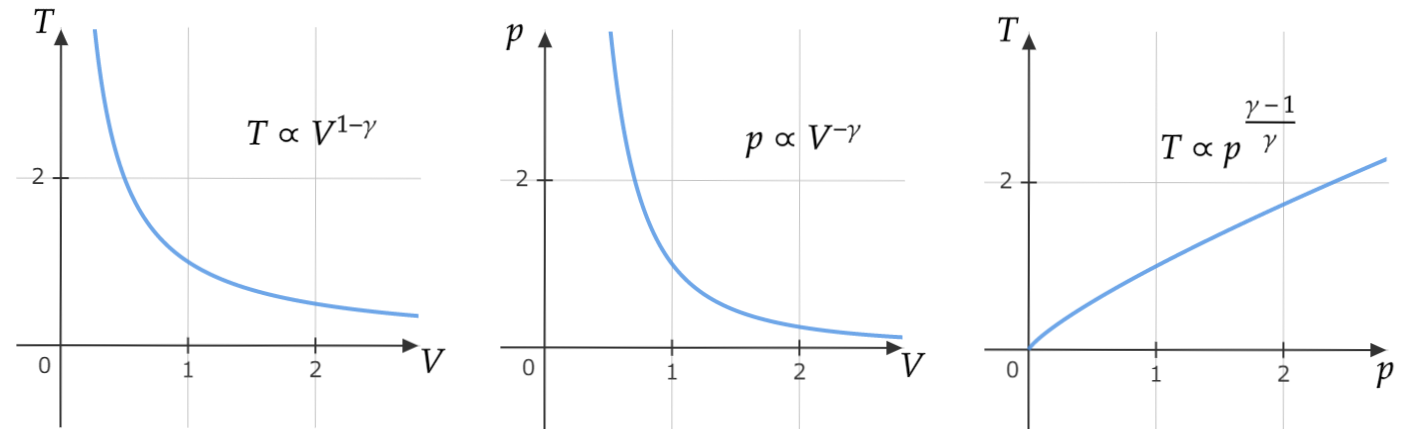
\includegraphics[scale = 0.4]{Images/AdiabaticIdealGas.png}
        \caption{Relationships for temperature, pressure, and volume for an adiabatic process involving an ideal gas.}
    \end{figure}
\end{eg}

Some specific applications of adiabatic processes are as follows: \begin{itemize}
    \item Diesel engine (spontaneous explosion due to heating; no spark plugs)
    \item Chinooks (air pressure increases due to lower altitude)
\end{itemize}



\begin{eg}[Black-body radiation]
    We now deal with electromagnetic radiation in a cavity in thermal equilibrium, which is emitted by black walls. Here ``black" means all radiation is absorbed:
    \begin{center}
        \begin{tikzpicture}[x=0.75pt,y=0.75pt,yscale=-1,xscale=1]
%uncomment if require: \path (0,398); %set diagram left start at 0, and has height of 398

%Shape: Rectangle [id:dp6362389483265465] 
\draw  [fill={rgb, 255:red, 253; green, 0; blue, 0 }  ,fill opacity=1 ][line width=2.25]  (100,126) -- (460,126) -- (460,306) -- (100,306) -- cycle ;
%Shape: Rectangle [id:dp03100105207175874] 
\draw  [color={rgb, 255:red, 0; green, 0; blue, 0 }  ,draw opacity=1 ][fill={rgb, 255:red, 255; green, 255; blue, 255 }  ,fill opacity=1 ][line width=2.25]  (190,171) -- (370,171) -- (370,261) -- (190,261) -- cycle ;

% Text Node
\draw (345,183.07) node [anchor=north west][inner sep=0.75pt]    {$V$};
% Text Node
\draw (443,280.07) node [anchor=north west][inner sep=0.75pt]    {$T$};
% Text Node
\draw (193,242.67) node [anchor=north west][inner sep=0.75pt]   [align=left] {Cavity};
% Text Node
\draw (102,286.67) node [anchor=north west][inner sep=0.75pt]   [align=left] {Heat Bath};


\end{tikzpicture}
    \end{center}
    Experiments show that $U = U(T,V) = V\epsilon(T)$, where $\epsilon$ is the energy density per volume. From classical electromagnetism, we also have $p = \frac{1}{3}\epsilon(T)$ for isotropic radiation (uniform radiation). The existence of a pressure from the classical perspective is similar to what we have for a gas. We can also borrow the wave-particle dualism from Quantum Mechanics. This suggests that we might be able to interpret or model black-body radiation as a \Emph{photon gas} (at least in a first approximation). Using our previous derivation for a gas we have \begin{equation*}
        C_V = \frac{\partial U}{\partial T} = V\frac{d\epsilon}{dT}
    \end{equation*}
    and for adiabats we find then \begin{equation*}
        \left(\frac{dT}{dV}\right)_{ad} = -\frac{p + \frac{\partial U}{\partial V}}{C_V} = -\frac{\frac{4}{3}\epsilon(T)}{V\frac{d\epsilon}{dT}}
    \end{equation*}
    We can rewrite this to obtain the simple ODE \begin{equation*}
        -\frac{d\epsilon}{\epsilon} = \frac{4}{3}\frac{dV}{V}
    \end{equation*}
    The solution of this ODE can be written as \begin{equation*}
        \epsilon V^{4/3} = const.
    \end{equation*}
    which has the equivalent form \begin{equation*}
        pV^{4/3} = const.
    \end{equation*}
    given the relationship between $p$ and $\epsilon$ for black-body radiation from above.
\end{eg}


Since no heat is flowing in or out of the system in an adiabatic process, in the absence of any friction we can completely recover the original state of the system by reversing the procedure. Such a process also converses entropy, as we will see later. 

\begin{defn}
    A thermodynamic process which is both adiabatic and reversible is said to be an \Emph{isentropic process}.
\end{defn}




\subsection{Isotherms}

\begin{defn}
    An \Emph{isotherm} is a change in the state of a system such that $dT = 0$.
\end{defn}

This is not to be confused with an adiabatic process in which there is no heat trnasfer between the surroundings and the system. $dT = 0$ relates to a level surface, or manifold, associated to a constant empirical temperature $\Theta$, which we use to define $T$.


%%%%%%%%%%%%%%%%%%%%%% Chapter 1.3
\chapter{Thermodynamical Engines and Refrigerators}


%%%%%%%%%%%%%%%%%%%% Section 1.3.1
\section{The 2nd Law of Thermodynamics}

Recall from the first law we know that energy is conserved during all thermodynamic processes. This leaves the question as to whether all thermodynamic processes that conserve energy can actually occur. To answer this we focus on the conversion of heat to work in terms of engines:

\begin{defn}
    An idealized \Emph{heat engine} is a thermodynamic system that runs in a \Emph{cycle} (i.e. it returns to the same internal thermodynamic states) taking in a certain amount of heat $Q_h$ from a heat bath with temperature $T_h$, converting a portion of it to work $W > 0$ and dumping the remaining heat $Q_c$ into a heat bath with $T_c < T_h$. The \Emph{efficiency} of a heat engine is given by \begin{equation}
        \eta = \frac{W}{Q_h} = \frac{Q_h-Q_c}{Q_h} = 1 - \frac{Q_c}{Q_h} \leq 1
    \end{equation}
\end{defn}

\begin{center}
    \begin{tikzpicture}[x=0.75pt,y=0.75pt,yscale=-1,xscale=1]
%uncomment if require: \path (0,288); %set diagram left start at 0, and has height of 288

%Shape: Circle [id:dp4831299922922003] 
\draw   (210,135) .. controls (210,110.15) and (230.15,90) .. (255,90) .. controls (279.85,90) and (300,110.15) .. (300,135) .. controls (300,159.85) and (279.85,180) .. (255,180) .. controls (230.15,180) and (210,159.85) .. (210,135) -- cycle ;
%Straight Lines [id:da9977923048639901] 
\draw    (255,50) -- (255,88) ;
\draw [shift={(255,90)}, rotate = 270] [color={rgb, 255:red, 0; green, 0; blue, 0 }  ][line width=0.75]    (10.93,-3.29) .. controls (6.95,-1.4) and (3.31,-0.3) .. (0,0) .. controls (3.31,0.3) and (6.95,1.4) .. (10.93,3.29)   ;
%Straight Lines [id:da745735751950716] 
\draw    (255,180) -- (255,218) ;
\draw [shift={(255,220)}, rotate = 270] [color={rgb, 255:red, 0; green, 0; blue, 0 }  ][line width=0.75]    (10.93,-3.29) .. controls (6.95,-1.4) and (3.31,-0.3) .. (0,0) .. controls (3.31,0.3) and (6.95,1.4) .. (10.93,3.29)   ;
%Straight Lines [id:da4282340901069286] 
\draw    (300,135) -- (368,135) ;
\draw [shift={(370,135)}, rotate = 180] [color={rgb, 255:red, 0; green, 0; blue, 0 }  ][line width=0.75]    (10.93,-3.29) .. controls (6.95,-1.4) and (3.31,-0.3) .. (0,0) .. controls (3.31,0.3) and (6.95,1.4) .. (10.93,3.29)   ;
%Rounded Rect [id:dp12016935374222504] 
\draw  [color={rgb, 255:red, 255; green, 0; blue, 0 }  ,draw opacity=1 ] (110,18) .. controls (110,13.58) and (113.58,10) .. (118,10) -- (392,10) .. controls (396.42,10) and (400,13.58) .. (400,18) -- (400,42) .. controls (400,46.42) and (396.42,50) .. (392,50) -- (118,50) .. controls (113.58,50) and (110,46.42) .. (110,42) -- cycle ;
%Rounded Rect [id:dp5253667581959272] 
\draw  [color={rgb, 255:red, 0; green, 139; blue, 255 }  ,draw opacity=1 ] (110,228) .. controls (110,223.58) and (113.58,220) .. (118,220) -- (392,220) .. controls (396.42,220) and (400,223.58) .. (400,228) -- (400,252) .. controls (400,256.42) and (396.42,260) .. (392,260) -- (118,260) .. controls (113.58,260) and (110,256.42) .. (110,252) -- cycle ;

% Text Node
\draw (380,12.4) node [anchor=north west][inner sep=0.75pt]    {$T_{h}$};
% Text Node
\draw (241,112.4) node [anchor=north west][inner sep=0.75pt]  [font=\huge]  {$E$};
% Text Node
\draw (257,62.4) node [anchor=north west][inner sep=0.75pt]  [color={rgb, 255:red, 255; green, 0; blue, 0 }  ,opacity=1 ]  {$Q_{h}$};
% Text Node
\draw (258,191.4) node [anchor=north west][inner sep=0.75pt]  [color={rgb, 255:red, 0; green, 135; blue, 255 }  ,opacity=1 ]  {$Q_{c}$};
% Text Node
\draw (331,113.4) node [anchor=north west][inner sep=0.75pt]    {$W$};
% Text Node
\draw (187,22) node [anchor=north west][inner sep=0.75pt]   [align=left] {{\fontfamily{ptm}\selectfont {\large Heat Bath (source) }}};
% Text Node
\draw (380,222.4) node [anchor=north west][inner sep=0.75pt]    {$T_{c}$};
% Text Node
\draw (194,232) node [anchor=north west][inner sep=0.75pt]   [align=left] {{\fontfamily{ptm}\selectfont {\large Heat Bath (sink) }}};


\end{tikzpicture}
\end{center}

\begin{defn}
    An idealized \Emph{refrigerator} can be considered as an idealized heat engine running backwards, such that it uses work $W$ to extract heat $Q_c$ (e.g. from an ice box) and dump the heat $Q_h$ at higher $T_h$ (e.g. through an exhaust). The \Emph{performance} of a refrigerator is given by \begin{equation}
        w = \frac{Q_c}{W} = \frac{Q_c}{Q_h-Q_c}
    \end{equation}
\end{defn}

\begin{center}
    \begin{tikzpicture}[x=0.75pt,y=0.75pt,yscale=-1,xscale=1]
%uncomment if require: \path (0,288); %set diagram left start at 0, and has height of 288

%Shape: Circle [id:dp4831299922922003] 
\draw   (210,135) .. controls (210,110.15) and (230.15,90) .. (255,90) .. controls (279.85,90) and (300,110.15) .. (300,135) .. controls (300,159.85) and (279.85,180) .. (255,180) .. controls (230.15,180) and (210,159.85) .. (210,135) -- cycle ;
%Straight Lines [id:da9977923048639901] 
\draw    (255,52) -- (255,90) ;
\draw [shift={(255,50)}, rotate = 90] [color={rgb, 255:red, 0; green, 0; blue, 0 }  ][line width=0.75]    (10.93,-3.29) .. controls (6.95,-1.4) and (3.31,-0.3) .. (0,0) .. controls (3.31,0.3) and (6.95,1.4) .. (10.93,3.29)   ;
%Straight Lines [id:da745735751950716] 
\draw    (255,182) -- (255,220) ;
\draw [shift={(255,180)}, rotate = 90] [color={rgb, 255:red, 0; green, 0; blue, 0 }  ][line width=0.75]    (10.93,-3.29) .. controls (6.95,-1.4) and (3.31,-0.3) .. (0,0) .. controls (3.31,0.3) and (6.95,1.4) .. (10.93,3.29)   ;
%Straight Lines [id:da4282340901069286] 
\draw    (140,135) -- (208,135) ;
\draw [shift={(210,135)}, rotate = 180] [color={rgb, 255:red, 0; green, 0; blue, 0 }  ][line width=0.75]    (10.93,-3.29) .. controls (6.95,-1.4) and (3.31,-0.3) .. (0,0) .. controls (3.31,0.3) and (6.95,1.4) .. (10.93,3.29)   ;
%Rounded Rect [id:dp12016935374222504] 
\draw  [color={rgb, 255:red, 255; green, 0; blue, 0 }  ,draw opacity=1 ] (110,18) .. controls (110,13.58) and (113.58,10) .. (118,10) -- (392,10) .. controls (396.42,10) and (400,13.58) .. (400,18) -- (400,42) .. controls (400,46.42) and (396.42,50) .. (392,50) -- (118,50) .. controls (113.58,50) and (110,46.42) .. (110,42) -- cycle ;
%Rounded Rect [id:dp5253667581959272] 
\draw  [color={rgb, 255:red, 0; green, 139; blue, 255 }  ,draw opacity=1 ] (110,228) .. controls (110,223.58) and (113.58,220) .. (118,220) -- (392,220) .. controls (396.42,220) and (400,223.58) .. (400,228) -- (400,252) .. controls (400,256.42) and (396.42,260) .. (392,260) -- (118,260) .. controls (113.58,260) and (110,256.42) .. (110,252) -- cycle ;
%Straight Lines [id:da01660900085043382] 
\draw    (140,130) -- (140,140) ;

% Text Node
\draw (380,12.4) node [anchor=north west][inner sep=0.75pt]    {$T_{h}$};
% Text Node
\draw (241,112.4) node [anchor=north west][inner sep=0.75pt]  [font=\huge]  {$R$};
% Text Node
\draw (257,62.4) node [anchor=north west][inner sep=0.75pt]  [color={rgb, 255:red, 255; green, 0; blue, 0 }  ,opacity=1 ]  {$Q_{h}$};
% Text Node
\draw (258,191.4) node [anchor=north west][inner sep=0.75pt]  [color={rgb, 255:red, 0; green, 135; blue, 255 }  ,opacity=1 ]  {$Q_{c}$};
% Text Node
\draw (152,113.4) node [anchor=north west][inner sep=0.75pt]    {$W$};
% Text Node
\draw (187,22) node [anchor=north west][inner sep=0.75pt]   [align=left] {{\fontfamily{ptm}\selectfont {\large Heat Bath (exhaust) }}};
% Text Node
\draw (380,222.4) node [anchor=north west][inner sep=0.75pt]    {$T_{c}$};
% Text Node
\draw (164,230) node [anchor=north west][inner sep=0.75pt]   [align=left] {{\fontfamily{ptm}\selectfont {\large Heat Bath (cold resevoir) }}};


\end{tikzpicture}
\end{center}

We will now give two formulations of the second law of thermodynamics:

\begin{law}[2nd Law of Thermodynamics (Kelvin)]
    A thermodynamic machine or process that runs in a cycle and whose sole result is the complete conversion of heat from a single heat bath or reservoir into work is not possible.
\end{law}

\begin{law}[2nd Law of Thermodynamics (Clausius)]
    There is no thermodynamics machine or process that runs in a cycle and whose sole result is the transfer of heat from a colder to a hotter body.
\end{law}

These two formulations are in fact equivalent, as we shall now prove:

\begin{proof}
    To prove their equivalence, we shall show ``not Kelvin" implies ``not Clausius" and vice-versa. First, suppose that there exists a thermodynamic machine that runs in a cycle and whose sole result is the complete conversion of heat from a single heat bath or reservoir into work. Let $T_h$ correspond to the reservoir of interest. Then, consider a refrigerator from a reservoir $T_c < T_h$ to $T_h$, and have the work come from our engine. Then, after the system as balanced, looking at the engine and refrigerator as a single machine we have that heat $Q_c$ comes from the cold reservoir, and heat $Q_h - Q_h'$ is deposited in the hot reservoir, without any external work. Thus, such a machine violates Clausius, as desired, and as shown in the following diagram:
        \begin{center}
            \begin{tikzpicture}[x=0.75pt,y=0.75pt,yscale=-1,xscale=1]
%uncomment if require: \path (0,288); %set diagram left start at 0, and has height of 288

%Shape: Circle [id:dp4831299922922003] 
\draw   (300.67,134.33) .. controls (300.67,109.48) and (320.81,89.33) .. (345.67,89.33) .. controls (370.52,89.33) and (390.67,109.48) .. (390.67,134.33) .. controls (390.67,159.19) and (370.52,179.33) .. (345.67,179.33) .. controls (320.81,179.33) and (300.67,159.19) .. (300.67,134.33) -- cycle ;
%Straight Lines [id:da9977923048639901] 
\draw    (345.67,51.33) -- (345.67,89.33) ;
\draw [shift={(345.67,49.33)}, rotate = 90] [color={rgb, 255:red, 0; green, 0; blue, 0 }  ][line width=0.75]    (10.93,-3.29) .. controls (6.95,-1.4) and (3.31,-0.3) .. (0,0) .. controls (3.31,0.3) and (6.95,1.4) .. (10.93,3.29)   ;
%Straight Lines [id:da745735751950716] 
\draw    (345.67,181.33) -- (345.67,219.33) ;
\draw [shift={(345.67,179.33)}, rotate = 90] [color={rgb, 255:red, 0; green, 0; blue, 0 }  ][line width=0.75]    (10.93,-3.29) .. controls (6.95,-1.4) and (3.31,-0.3) .. (0,0) .. controls (3.31,0.3) and (6.95,1.4) .. (10.93,3.29)   ;
%Straight Lines [id:da4282340901069286] 
\draw    (230.67,134.33) -- (298.67,134.33) ;
\draw [shift={(300.67,134.33)}, rotate = 180] [color={rgb, 255:red, 0; green, 0; blue, 0 }  ][line width=0.75]    (10.93,-3.29) .. controls (6.95,-1.4) and (3.31,-0.3) .. (0,0) .. controls (3.31,0.3) and (6.95,1.4) .. (10.93,3.29)   ;
%Rounded Rect [id:dp12016935374222504] 
\draw  [color={rgb, 255:red, 255; green, 0; blue, 0 }  ,draw opacity=1 ] (110,18) .. controls (110,13.58) and (113.58,10) .. (118,10) -- (392,10) .. controls (396.42,10) and (400,13.58) .. (400,18) -- (400,42) .. controls (400,46.42) and (396.42,50) .. (392,50) -- (118,50) .. controls (113.58,50) and (110,46.42) .. (110,42) -- cycle ;
%Rounded Rect [id:dp5253667581959272] 
\draw  [color={rgb, 255:red, 0; green, 139; blue, 255 }  ,draw opacity=1 ] (110,228) .. controls (110,223.58) and (113.58,220) .. (118,220) -- (392,220) .. controls (396.42,220) and (400,223.58) .. (400,228) -- (400,252) .. controls (400,256.42) and (396.42,260) .. (392,260) -- (118,260) .. controls (113.58,260) and (110,256.42) .. (110,252) -- cycle ;
%Straight Lines [id:da01660900085043382] 
\draw    (230.67,129.33) -- (230.67,139.33) ;
%Shape: Circle [id:dp9583179343344637] 
\draw   (140.67,134.33) .. controls (140.67,109.48) and (160.81,89.33) .. (185.67,89.33) .. controls (210.52,89.33) and (230.67,109.48) .. (230.67,134.33) .. controls (230.67,159.19) and (210.52,179.33) .. (185.67,179.33) .. controls (160.81,179.33) and (140.67,159.19) .. (140.67,134.33) -- cycle ;
%Straight Lines [id:da5396194960167366] 
\draw    (185,50) -- (185,88) ;
\draw [shift={(185,90)}, rotate = 270] [color={rgb, 255:red, 0; green, 0; blue, 0 }  ][line width=0.75]    (10.93,-3.29) .. controls (6.95,-1.4) and (3.31,-0.3) .. (0,0) .. controls (3.31,0.3) and (6.95,1.4) .. (10.93,3.29)   ;
%Rounded Rect [id:dp6223483168411648] 
\draw  [color={rgb, 255:red, 85; green, 199; blue, 11 }  ,draw opacity=1 ] (110,102) .. controls (110,89.85) and (119.85,80) .. (132,80) -- (398,80) .. controls (410.15,80) and (420,89.85) .. (420,102) -- (420,168) .. controls (420,180.15) and (410.15,190) .. (398,190) -- (132,190) .. controls (119.85,190) and (110,180.15) .. (110,168) -- cycle ;

% Text Node
\draw (380,12.4) node [anchor=north west][inner sep=0.75pt]    {$T_{h}$};
% Text Node
\draw (331.67,111.73) node [anchor=north west][inner sep=0.75pt]  [font=\huge]  {$R$};
% Text Node
\draw (347.67,61.73) node [anchor=north west][inner sep=0.75pt]  [color={rgb, 255:red, 255; green, 0; blue, 0 }  ,opacity=1 ]  {$Q_{h}$};
% Text Node
\draw (348.67,190.73) node [anchor=north west][inner sep=0.75pt]  [color={rgb, 255:red, 0; green, 135; blue, 255 }  ,opacity=1 ]  {$Q_{c}$};
% Text Node
\draw (261,142.4) node [anchor=north west][inner sep=0.75pt]    {$W$};
% Text Node
\draw (181,22) node [anchor=north west][inner sep=0.75pt]   [align=left] {{\fontfamily{ptm}\selectfont {\large Heat Bath (hot resevoir) }}};
% Text Node
\draw (380,222.4) node [anchor=north west][inner sep=0.75pt]    {$T_{c}$};
% Text Node
\draw (164,230) node [anchor=north west][inner sep=0.75pt]   [align=left] {{\fontfamily{ptm}\selectfont {\large Heat Bath (cold resevoir) }}};
% Text Node
\draw (187,62.4) node [anchor=north west][inner sep=0.75pt]  [color={rgb, 255:red, 255; green, 0; blue, 0 }  ,opacity=1 ]  {$Q'_{h}$};
% Text Node
\draw (171,103.4) node [anchor=north west][inner sep=0.75pt]  [font=\huge]  {$\overline{K}$};
% Text Node
\draw (250,83.4) node [anchor=north west][inner sep=0.75pt]  [font=\huge]  {$\overline{C}$};


\end{tikzpicture}
        \end{center}
        Next, suppose there exists a thermodynamic machine that runs in a cycle and whose sole result is the transfer of heat, $Q$, from a colder to a hotter body. Then, connect an engine that takes heat $Q_h$ from the hotter body, does work $W$, and deposits heat $Q_c$ to the colder body. It follows that the combined machine has input $Q_h - Q$ from the hot body, work output $W$, and heat output $Q_c - Q$. We then adjust the output of the heat engine such that $Q_c = Q$. Then we have obtained a machine violating Kelvin, as seen in the diagram:

        \begin{center}
            \begin{tikzpicture}[x=0.75pt,y=0.75pt,yscale=-1,xscale=1]
%uncomment if require: \path (0,288); %set diagram left start at 0, and has height of 288

%Shape: Circle [id:dp4831299922922003] 
\draw   (300.67,134.33) .. controls (300.67,109.48) and (320.81,89.33) .. (345.67,89.33) .. controls (370.52,89.33) and (390.67,109.48) .. (390.67,134.33) .. controls (390.67,159.19) and (370.52,179.33) .. (345.67,179.33) .. controls (320.81,179.33) and (300.67,159.19) .. (300.67,134.33) -- cycle ;
%Straight Lines [id:da9977923048639901] 
\draw    (345.67,49.33) -- (345.67,87.33) ;
\draw [shift={(345.67,89.33)}, rotate = 270] [color={rgb, 255:red, 0; green, 0; blue, 0 }  ][line width=0.75]    (10.93,-3.29) .. controls (6.95,-1.4) and (3.31,-0.3) .. (0,0) .. controls (3.31,0.3) and (6.95,1.4) .. (10.93,3.29)   ;
%Straight Lines [id:da745735751950716] 
\draw    (185,182) -- (185,220) ;
\draw [shift={(185,180)}, rotate = 90] [color={rgb, 255:red, 0; green, 0; blue, 0 }  ][line width=0.75]    (10.93,-3.29) .. controls (6.95,-1.4) and (3.31,-0.3) .. (0,0) .. controls (3.31,0.3) and (6.95,1.4) .. (10.93,3.29)   ;
%Straight Lines [id:da4282340901069286] 
\draw    (390.67,134.33) -- (458.67,134.33) ;
\draw [shift={(460.67,134.33)}, rotate = 180] [color={rgb, 255:red, 0; green, 0; blue, 0 }  ][line width=0.75]    (10.93,-3.29) .. controls (6.95,-1.4) and (3.31,-0.3) .. (0,0) .. controls (3.31,0.3) and (6.95,1.4) .. (10.93,3.29)   ;
%Rounded Rect [id:dp12016935374222504] 
\draw  [color={rgb, 255:red, 255; green, 0; blue, 0 }  ,draw opacity=1 ] (110,18) .. controls (110,13.58) and (113.58,10) .. (118,10) -- (392,10) .. controls (396.42,10) and (400,13.58) .. (400,18) -- (400,42) .. controls (400,46.42) and (396.42,50) .. (392,50) -- (118,50) .. controls (113.58,50) and (110,46.42) .. (110,42) -- cycle ;
%Rounded Rect [id:dp5253667581959272] 
\draw  [color={rgb, 255:red, 0; green, 139; blue, 255 }  ,draw opacity=1 ] (110,228) .. controls (110,223.58) and (113.58,220) .. (118,220) -- (392,220) .. controls (396.42,220) and (400,223.58) .. (400,228) -- (400,252) .. controls (400,256.42) and (396.42,260) .. (392,260) -- (118,260) .. controls (113.58,260) and (110,256.42) .. (110,252) -- cycle ;
%Straight Lines [id:da01660900085043382] 
\draw    (230.67,129.33) -- (230.67,139.33) ;
%Shape: Circle [id:dp9583179343344637] 
\draw   (140.67,134.33) .. controls (140.67,109.48) and (160.81,89.33) .. (185.67,89.33) .. controls (210.52,89.33) and (230.67,109.48) .. (230.67,134.33) .. controls (230.67,159.19) and (210.52,179.33) .. (185.67,179.33) .. controls (160.81,179.33) and (140.67,159.19) .. (140.67,134.33) -- cycle ;
%Straight Lines [id:da5396194960167366] 
\draw    (185,52) -- (185,90) ;
\draw [shift={(185,50)}, rotate = 90] [color={rgb, 255:red, 0; green, 0; blue, 0 }  ][line width=0.75]    (10.93,-3.29) .. controls (6.95,-1.4) and (3.31,-0.3) .. (0,0) .. controls (3.31,0.3) and (6.95,1.4) .. (10.93,3.29)   ;
%Rounded Rect [id:dp6223483168411648] 
\draw  [color={rgb, 255:red, 85; green, 199; blue, 11 }  ,draw opacity=1 ] (110,102) .. controls (110,89.85) and (119.85,80) .. (132,80) -- (398,80) .. controls (410.15,80) and (420,89.85) .. (420,102) -- (420,168) .. controls (420,180.15) and (410.15,190) .. (398,190) -- (132,190) .. controls (119.85,190) and (110,180.15) .. (110,168) -- cycle ;
%Straight Lines [id:da8097853550719598] 
\draw    (345.67,179.33) -- (345.67,217.33) ;
\draw [shift={(345.67,219.33)}, rotate = 270] [color={rgb, 255:red, 0; green, 0; blue, 0 }  ][line width=0.75]    (10.93,-3.29) .. controls (6.95,-1.4) and (3.31,-0.3) .. (0,0) .. controls (3.31,0.3) and (6.95,1.4) .. (10.93,3.29)   ;

% Text Node
\draw (380,12.4) node [anchor=north west][inner sep=0.75pt]    {$T_{h}$};
% Text Node
\draw (331.67,111.73) node [anchor=north west][inner sep=0.75pt]  [font=\huge]  {$E$};
% Text Node
\draw (347.67,61.73) node [anchor=north west][inner sep=0.75pt]  [color={rgb, 255:red, 255; green, 0; blue, 0 }  ,opacity=1 ]  {$Q_{h}$};
% Text Node
\draw (188,191.4) node [anchor=north west][inner sep=0.75pt]  [color={rgb, 255:red, 0; green, 135; blue, 255 }  ,opacity=1 ]  {$Q$};
% Text Node
\draw (401,113.4) node [anchor=north west][inner sep=0.75pt]    {$W$};
% Text Node
\draw (181,22) node [anchor=north west][inner sep=0.75pt]   [align=left] {{\fontfamily{ptm}\selectfont {\large Heat Bath (hot resevoir) }}};
% Text Node
\draw (380,222.4) node [anchor=north west][inner sep=0.75pt]    {$T_{c}$};
% Text Node
\draw (164,230) node [anchor=north west][inner sep=0.75pt]   [align=left] {{\fontfamily{ptm}\selectfont {\large Heat Bath (cold resevoir) }}};
% Text Node
\draw (187,62.4) node [anchor=north west][inner sep=0.75pt]  [color={rgb, 255:red, 255; green, 0; blue, 0 }  ,opacity=1 ]  {$Q$};
% Text Node
\draw (171,103.4) node [anchor=north west][inner sep=0.75pt]  [font=\huge]  {$\overline{C}$};
% Text Node
\draw (250,83.4) node [anchor=north west][inner sep=0.75pt]  [font=\huge]  {$\overline{K}$};
% Text Node
\draw (351,192.4) node [anchor=north west][inner sep=0.75pt]  [color={rgb, 255:red, 0; green, 135; blue, 255 }  ,opacity=1 ]  {$Q$};


\end{tikzpicture}
        \end{center}
\end{proof}




%%%%%%%%%%%%%%%%%%%% Section 1.3.2
\section{Carnot Engines}

We now investigate the idea of the most efficient heat engine. 

\begin{defn}
    A \Emph{Carnot engine} is any heat engine that is reversible and runs in a cycle along two isotherms at temperatures $T_h$ and $T_c$ and adiabats. A \Emph{reversible} process is one that can be run backward in time by simply reversing its inputs and outputs. 
\end{defn}

\begin{eg}[Carnot Engine with an Ideal Gas as the Internal Working Substance]
    Here we have adiabatic compression of the gas, causing $\Delta T = T_h - T_c > 0$ ($A\rightarrow B$), then we have isothermal expansion with $\Delta Q_1 = Q_h > 0$ ($B\rightarrow C$), next we have adiabatic expansion which causes $\Delta T = T_c - T_h < 0$ ($C\rightarrow D$), and finally isothermal compression with $\Delta Q_2 = -Q_c < 0$ ($D\rightarrow A$).
    \begin{center}
        \begin{tikzpicture}[x=0.75pt,y=0.75pt,yscale=-1,xscale=1]
%uncomment if require: \path (0,288); %set diagram left start at 0, and has height of 288

%Shape: Right Angle [id:dp843558691918219] 
\draw   (370,220) -- (160,220) -- (160,40) ;
\draw   (156.71,47) -- (160.19,40.22) -- (163.67,47) ;
\draw   (363.3,216.63) -- (370.08,220.11) -- (363.3,223.59) ;
%Curve Lines [id:da8766430669684191] 
\draw    (209.33,109.33) .. controls (219.83,118.08) and (254.83,150.08) .. (309.83,150.08) ;
\draw [shift={(256.04,139.25)}, rotate = 203.76] [color={rgb, 255:red, 0; green, 0; blue, 0 }  ][line width=0.75]    (10.93,-3.29) .. controls (6.95,-1.4) and (3.31,-0.3) .. (0,0) .. controls (3.31,0.3) and (6.95,1.4) .. (10.93,3.29)   ;
%Curve Lines [id:da47282664716897016] 
\draw    (226.33,175.08) .. controls (236.83,183.83) and (275.83,199.58) .. (330.83,199.58) ;
\draw [shift={(276.99,194.27)}, rotate = 12.33] [color={rgb, 255:red, 0; green, 0; blue, 0 }  ][line width=0.75]    (10.93,-3.29) .. controls (6.95,-1.4) and (3.31,-0.3) .. (0,0) .. controls (3.31,0.3) and (6.95,1.4) .. (10.93,3.29)   ;
%Curve Lines [id:da19308737717293245] 
\draw  [dash pattern={on 4.5pt off 4.5pt}]  (206.83,79.75) .. controls (206.83,111.75) and (219.33,165.92) .. (240.83,213.92) ;
\draw [shift={(217.79,148.67)}, rotate = 75.43] [color={rgb, 255:red, 0; green, 0; blue, 0 }  ][line width=0.75]    (10.93,-3.29) .. controls (6.95,-1.4) and (3.31,-0.3) .. (0,0) .. controls (3.31,0.3) and (6.95,1.4) .. (10.93,3.29)   ;
%Curve Lines [id:da4455351667362961] 
\draw  [dash pattern={on 4.5pt off 4.5pt}]  (302.83,108.75) .. controls (302.83,140.75) and (316.33,166.92) .. (337.83,214.92) ;
\draw [shift={(315.18,163.42)}, rotate = 248.82999999999998] [color={rgb, 255:red, 0; green, 0; blue, 0 }  ][line width=0.75]    (10.93,-3.29) .. controls (6.95,-1.4) and (3.31,-0.3) .. (0,0) .. controls (3.31,0.3) and (6.95,1.4) .. (10.93,3.29)   ;
%Straight Lines [id:da7064223462049448] 
\draw    (245.6,121.88) -- (237.34,134.97)(243.07,120.28) -- (234.8,133.36) ;
\draw [shift={(232.33,140.08)}, rotate = 302.28] [color={rgb, 255:red, 0; green, 0; blue, 0 }  ][line width=0.75]    (8.74,-3.92) .. controls (5.56,-1.84) and (2.65,-0.53) .. (0,0) .. controls (2.65,0.53) and (5.56,1.84) .. (8.74,3.92)   ;
%Straight Lines [id:da05642770961721699] 
\draw [line width=0.75]    (273.1,185.88) -- (264.84,198.97)(270.57,184.28) -- (262.3,197.36) ;
\draw [shift={(259.83,204.08)}, rotate = 302.28] [color={rgb, 255:red, 0; green, 0; blue, 0 }  ][line width=0.75]    (8.74,-3.92) .. controls (5.56,-1.84) and (2.65,-0.53) .. (0,0) .. controls (2.65,0.53) and (5.56,1.84) .. (8.74,3.92)   ;
%Curve Lines [id:da10018836511051932] 
\draw  [dash pattern={on 4.5pt off 4.5pt}]  (189.83,73.75) .. controls (204.33,135.75) and (298.33,161.25) .. (345.33,146.75) ;
%Curve Lines [id:da2569141398168828] 
\draw  [dash pattern={on 4.5pt off 4.5pt}]  (192.83,146.75) .. controls (233.33,200.25) and (319.33,205.75) .. (385.33,196.25) ;

% Text Node
\draw (145.33,35.73) node [anchor=north west][inner sep=0.75pt]    {$P$};
% Text Node
\draw (373.33,215.23) node [anchor=north west][inner sep=0.75pt]    {$V$};
% Text Node
\draw (246.83,112.73) node [anchor=north west][inner sep=0.75pt]  [font=\scriptsize]  {$Q_{h}$};
% Text Node
\draw (274.33,177.73) node [anchor=north west][inner sep=0.75pt]  [font=\scriptsize]  {$Q_{c}$};
% Text Node
\draw (214.83,175.07) node [anchor=north west][inner sep=0.75pt]  [font=\scriptsize]  {$A$};
% Text Node
\draw (198.33,108.07) node [anchor=north west][inner sep=0.75pt]  [font=\scriptsize]  {$B$};
% Text Node
\draw (310.83,135.57) node [anchor=north west][inner sep=0.75pt]  [font=\scriptsize]  {$C$};
% Text Node
\draw (340.33,203.57) node [anchor=north west][inner sep=0.75pt]  [font=\scriptsize]  {$D$};
% Text Node
\draw (184.83,65.4) node [anchor=north west][inner sep=0.75pt]  [font=\scriptsize]  {$\delta Q=0$};
% Text Node
\draw (278.83,93.9) node [anchor=north west][inner sep=0.75pt]  [font=\scriptsize]  {$\delta Q=0$};
% Text Node
\draw (344.83,139.9) node [anchor=north west][inner sep=0.75pt]  [font=\scriptsize]  {$T_{h}$};
% Text Node
\draw (385.83,188.9) node [anchor=north west][inner sep=0.75pt]  [font=\scriptsize]  {$T_{c}$};

\draw   (209.36, 109.08) circle [x radius= 5, y radius= 5]   ;
\draw   (310.43, 150.62) circle [x radius= 5, y radius= 5]   ;
\draw   (238.15, 130.88) circle [x radius= 5, y radius= 5]   ;
\end{tikzpicture}
    \end{center}
    Over one cycle, the 1st law gives us \begin{equation*}
        0 = \oint dU = \Delta Q_1 + \Delta Q_2 + \Delta W
    \end{equation*}
    We calculate $\Delta W$ by considering the individual contributions: \begin{itemize}
        \item $A\rightarrow B$: adiabatic process, so $\delta Q = 0$, and $\delta W = dU$. Hence, $\Delta W_{AB} = U(T_h) - U(T_c)$, where we have used that $U = U(T)$ for an ideal gas.
        \item $B\rightarrow C$: isomethermal process, so $dT = 0$. Hence, $p = p(V)$ for an ideal gas in a closed system setting ($pV = Nk_BT$) as temperature is a constant, and so $$\Delta W_{BC} = -\int_B^Cp(V)dV = -Nk_BT_h\int_{V_B}^{V_C}\frac{dV}{V} = -Nk_BT_h\ln\frac{V_C}{V_B}$$
        \item $C\rightarrow D$: another adiabatic process, so $\Delta W_{CD} = U(T_c) - U(T_h)$ as in $A\rightarrow B$
        \item $D\rightarrow A$: another isothermal process, so $\Delta W_{DA} = -Nk_BT_c\ln\frac{V_A}{V_D}$ as in $B\rightarrow C$
    \end{itemize}
    This gives the total work: \begin{equation*}
        \Delta W = \Delta W_{AB} + \Delta W_{BC} + \Delta W_{CD} + \Delta W_{DA} = -Nk_B\left(T_h\ln\frac{V_C}{V_B} +T_c\ln\frac{V_A}{V_D}\right)
    \end{equation*}
    Recall that since we are dealing with adiabats, we have $TV^{\gamma -1} = const$, where the constant is the same along a given adiabat. This implies that $T_hV_B^{\gamma - 1} = T_cV_A^{\gamma -1}$ and $T_hV_C^{\gamma - 1} = T_cV_D^{\gamma - 1}$. Dividing the first equation by the second and simplifying slightly gives $\frac{V_B}{V_C} = \frac{V_A}{V_D}$. Using this in the above equation we find \begin{equation*}
        \Delta W = -Nk_B\ln\frac{V_D}{V_A}(T_h - T_c) < 0
    \end{equation*}
    Now, by definition the efficiency of a Carnot engine for an ideal gas is \begin{equation*}
        \eta_{C,ideal\;gas} = \frac{W}{Q_h} = \frac{-\Delta W}{\Delta Q_1}
    \end{equation*}
    Now, since $U = U(T)$ for an ideal gas in a closed system, we have $\Delta U = 0$ for any isothermal process. Thus, during the isothermal expansion the 1st law gives us \begin{equation*}
        \Delta Q_1 = -\Delta W_{BC} = Nk_BT_h\ln\frac{V_D}{V_A} > 0
    \end{equation*}
    using the identity between volume ratios $\frac{V_B}{V_C} = \frac{V_A}{V_D}$. Using the expressions for $\Delta W$ and $\Delta Q_1$, we obtain the efficiency \begin{equation*}
        \eta_{C,ideal\;gas} = \frac{W}{Q_h} = \frac{-\Delta W}{\Delta Q_1} = 1 - \frac{T_c}{T_h}
    \end{equation*}
\end{eg}

\subsection{Carnot's Theorem}

We can now address the question of which heat engine is the most efficient: 

\begin{namthm}[Carnot's Theorem]
    No heat engine operating between two heat reservoirs (at temperatures $T_h$ and $T_c$) is more efficient than a Carnot engine operating between them.
\end{namthm}
\begin{proof}
    We start with any given heat engine and couple it with a Carnot engine, which is run in reverse as a refrigerator and powerd by the other engine:
    \begin{center}
        \begin{tikzpicture}[x=0.75pt,y=0.75pt,yscale=-1,xscale=1]
%uncomment if require: \path (0,288); %set diagram left start at 0, and has height of 288

%Rounded Rect [id:dp38561762820116385] 
\draw  [color={rgb, 255:red, 255; green, 0; blue, 0 }  ,draw opacity=1 ] (185,20.91) .. controls (185,15.44) and (189.44,11) .. (194.91,11) -- (447.98,11) .. controls (453.45,11) and (457.89,15.44) .. (457.89,20.91) -- (457.89,50.64) .. controls (457.89,56.12) and (453.45,60.56) .. (447.98,60.56) -- (194.91,60.56) .. controls (189.44,60.56) and (185,56.12) .. (185,50.64) -- cycle ;
%Rounded Rect [id:dp11614062251907709] 
\draw  [color={rgb, 255:red, 0; green, 148; blue, 255 }  ,draw opacity=1 ] (185,206.24) .. controls (185,200.77) and (189.44,196.33) .. (194.91,196.33) -- (447.98,196.33) .. controls (453.45,196.33) and (457.89,200.77) .. (457.89,206.24) -- (457.89,235.98) .. controls (457.89,241.45) and (453.45,245.89) .. (447.98,245.89) -- (194.91,245.89) .. controls (189.44,245.89) and (185,241.45) .. (185,235.98) -- cycle ;
%Shape: Circle [id:dp5999093300147897] 
\draw   (228.22,130.5) .. controls (228.22,113.29) and (242.18,99.33) .. (259.39,99.33) .. controls (276.6,99.33) and (290.56,113.29) .. (290.56,130.5) .. controls (290.56,147.71) and (276.6,161.67) .. (259.39,161.67) .. controls (242.18,161.67) and (228.22,147.71) .. (228.22,130.5) -- cycle ;
%Shape: Circle [id:dp007932259288887522] 
\draw   (351.56,131.17) .. controls (351.56,113.95) and (365.51,100) .. (382.72,100) .. controls (399.94,100) and (413.89,113.95) .. (413.89,131.17) .. controls (413.89,148.38) and (399.94,162.33) .. (382.72,162.33) .. controls (365.51,162.33) and (351.56,148.38) .. (351.56,131.17) -- cycle ;
%Straight Lines [id:da7447172424421336] 
\draw    (259.4,60) -- (259.39,97.33) ;
\draw [shift={(259.39,99.33)}, rotate = 270.02] [color={rgb, 255:red, 0; green, 0; blue, 0 }  ][line width=0.75]    (10.93,-3.29) .. controls (6.95,-1.4) and (3.31,-0.3) .. (0,0) .. controls (3.31,0.3) and (6.95,1.4) .. (10.93,3.29)   ;
%Straight Lines [id:da21237543507400014] 
\draw    (382.73,62.67) -- (382.72,100) ;
\draw [shift={(382.73,60.67)}, rotate = 90.02] [color={rgb, 255:red, 0; green, 0; blue, 0 }  ][line width=0.75]    (10.93,-3.29) .. controls (6.95,-1.4) and (3.31,-0.3) .. (0,0) .. controls (3.31,0.3) and (6.95,1.4) .. (10.93,3.29)   ;
%Straight Lines [id:da523718903355215] 
\draw    (382.72,164.33) -- (382.71,196) ;
\draw [shift={(382.72,162.33)}, rotate = 90.02] [color={rgb, 255:red, 0; green, 0; blue, 0 }  ][line width=0.75]    (10.93,-3.29) .. controls (6.95,-1.4) and (3.31,-0.3) .. (0,0) .. controls (3.31,0.3) and (6.95,1.4) .. (10.93,3.29)   ;
%Straight Lines [id:da4858891627092614] 
\draw    (259.39,161.67) -- (259.38,193.33) ;
\draw [shift={(259.38,195.33)}, rotate = 270.02] [color={rgb, 255:red, 0; green, 0; blue, 0 }  ][line width=0.75]    (10.93,-3.29) .. controls (6.95,-1.4) and (3.31,-0.3) .. (0,0) .. controls (3.31,0.3) and (6.95,1.4) .. (10.93,3.29)   ;
%Straight Lines [id:da4063459383288237] 
\draw    (290.56,130.5) -- (349.56,131.14) ;
\draw [shift={(351.56,131.17)}, rotate = 180.63] [color={rgb, 255:red, 0; green, 0; blue, 0 }  ][line width=0.75]    (10.93,-3.29) .. controls (6.95,-1.4) and (3.31,-0.3) .. (0,0) .. controls (3.31,0.3) and (6.95,1.4) .. (10.93,3.29)   ;

% Text Node
\draw (435.56,10.73) node [anchor=north west][inner sep=0.75pt]    {$T_{h}$};
% Text Node
\draw (435.56,197.73) node [anchor=north west][inner sep=0.75pt]    {$T_{c}$};
% Text Node
\draw (244.89,121.73) node [anchor=north west][inner sep=0.75pt]    {$\neg C$};
% Text Node
\draw (376.89,121.73) node [anchor=north west][inner sep=0.75pt]    {$C$};
% Text Node
\draw (311,113.4) node [anchor=north west][inner sep=0.75pt]    {$W$};
% Text Node
\draw (261,72.4) node [anchor=north west][inner sep=0.75pt]    {$Q_{h}$};
% Text Node
\draw (387,72.4) node [anchor=north west][inner sep=0.75pt]    {$Q'_{h}$};
% Text Node
\draw (261.39,165.07) node [anchor=north west][inner sep=0.75pt]    {$Q_{c}$};
% Text Node
\draw (387,171.4) node [anchor=north west][inner sep=0.75pt]    {$Q'_{c}$};
% Text Node
\draw (247,32) node [anchor=north west][inner sep=0.75pt]  [color={rgb, 255:red, 255; green, 0; blue, 0 }  ,opacity=1 ] [align=left] {{\fontfamily{ptm}\selectfont Heat Bath (hot reservoir)}};
% Text Node
\draw (247,212) node [anchor=north west][inner sep=0.75pt]  [color={rgb, 255:red, 0; green, 144; blue, 255 }  ,opacity=1 ] [align=left] {{\fontfamily{ptm}\selectfont Heat Bath (cold reservoir)}};


\end{tikzpicture}
    \end{center}
    Instead of considering both engines in isolation, we can equivalently consider them as a combined engine, taking in heat $Q_h - Q_h'$, and outputing heat $Q_c - Q_c'$. As this combined machine runs in a cycle, so $\Delta U = 0$ over a cycle, and only exchanges heat with the outside world without doing any external work, we have $Q_h + Q_c' = Q_c + Q_h'$ based on the first law of thermodynamics. Moreover, the combined machine falls under the 2nd law of thermodynamics. Using the formulation by Clausius, we have $Q_h - Q_h' \geq 0$, so $Q_h \geq Q_h'$, and hence $\frac{W}{Q_h} \leq \frac{W}{Q_h'}$. This implies that $\eta \leq \eta_C$ (where the last implication uses the fact that Carnot engines are exactly reversible).
\end{proof}

\begin{cor}
    All reversible engines have the same universal efficiency $\eta = \eta_C(T_h,T_c) = 1-\frac{T_c}{T_h}$.
\end{cor}
\begin{proof}
    Each reversible Carnot engine can be used to run any other reversible heat engine backwards.
\end{proof}



%%%%%%%%%%%%%%%%%%%% Section 1.3.3
\section{Thermodynamic Temperature Scale}


Recall the $0$th law ensures the existence of a temperature. For the ideal gas we can use the equation of state to define $T$, but this does not usually genrealize to other systems. We now use the universal efficiency $\eta_C$ of Carnot engines to establish a more general thermodynamic temperature scale. Consider two coupled Carnot engines with some empirical temperature scale $\Theta$: 
\begin{center}
    \begin{tikzpicture}[x=0.75pt,y=0.75pt,yscale=-1,xscale=1]
%uncomment if require: \path (0,294); %set diagram left start at 0, and has height of 294

%Straight Lines [id:da05453093434369749] 
\draw    (60,12) -- (240,12) ;
%Straight Lines [id:da6200862679386634] 
\draw    (60,144) -- (240,144) ;
%Straight Lines [id:da706189415713308] 
\draw    (60,276) -- (240,276) ;
%Rounded Rect [id:dp4036699475049652] 
\draw  [fill={rgb, 255:red, 136; green, 255; blue, 0 }  ,fill opacity=1 ] (96,57.6) .. controls (96,52.3) and (100.3,48) .. (105.6,48) -- (194.4,48) .. controls (199.7,48) and (204,52.3) .. (204,57.6) -- (204,86.4) .. controls (204,91.7) and (199.7,96) .. (194.4,96) -- (105.6,96) .. controls (100.3,96) and (96,91.7) .. (96,86.4) -- cycle ;
%Rounded Rect [id:dp37939651638989935] 
\draw  [fill={rgb, 255:red, 255; green, 0; blue, 0 }  ,fill opacity=1 ] (96,201.6) .. controls (96,196.3) and (100.3,192) .. (105.6,192) -- (194.4,192) .. controls (199.7,192) and (204,196.3) .. (204,201.6) -- (204,230.4) .. controls (204,235.7) and (199.7,240) .. (194.4,240) -- (105.6,240) .. controls (100.3,240) and (96,235.7) .. (96,230.4) -- cycle ;
%Straight Lines [id:da7142280284189315] 
\draw    (150,12) -- (150,46) ;
\draw [shift={(150,48)}, rotate = 270] [color={rgb, 255:red, 0; green, 0; blue, 0 }  ][line width=0.75]    (10.93,-3.29) .. controls (6.95,-1.4) and (3.31,-0.3) .. (0,0) .. controls (3.31,0.3) and (6.95,1.4) .. (10.93,3.29)   ;
%Straight Lines [id:da0985311285686783] 
\draw    (150,96) -- (150,142) ;
\draw [shift={(150,144)}, rotate = 270] [color={rgb, 255:red, 0; green, 0; blue, 0 }  ][line width=0.75]    (10.93,-3.29) .. controls (6.95,-1.4) and (3.31,-0.3) .. (0,0) .. controls (3.31,0.3) and (6.95,1.4) .. (10.93,3.29)   ;
%Straight Lines [id:da5535079418179869] 
\draw    (150,144) -- (150,190) ;
\draw [shift={(150,192)}, rotate = 270] [color={rgb, 255:red, 0; green, 0; blue, 0 }  ][line width=0.75]    (10.93,-3.29) .. controls (6.95,-1.4) and (3.31,-0.3) .. (0,0) .. controls (3.31,0.3) and (6.95,1.4) .. (10.93,3.29)   ;
%Straight Lines [id:da3167310910998773] 
\draw    (150,240) -- (150,274) ;
\draw [shift={(150,276)}, rotate = 270] [color={rgb, 255:red, 0; green, 0; blue, 0 }  ][line width=0.75]    (10.93,-3.29) .. controls (6.95,-1.4) and (3.31,-0.3) .. (0,0) .. controls (3.31,0.3) and (6.95,1.4) .. (10.93,3.29)   ;
%Straight Lines [id:da576279060400507] 
\draw    (204,72) -- (250,72) ;
\draw [shift={(252,72)}, rotate = 180] [color={rgb, 255:red, 0; green, 0; blue, 0 }  ][line width=0.75]    (10.93,-3.29) .. controls (6.95,-1.4) and (3.31,-0.3) .. (0,0) .. controls (3.31,0.3) and (6.95,1.4) .. (10.93,3.29)   ;
%Straight Lines [id:da8007473356697774] 
\draw    (204,216) -- (250,216) ;
\draw [shift={(252,216)}, rotate = 180] [color={rgb, 255:red, 0; green, 0; blue, 0 }  ][line width=0.75]    (10.93,-3.29) .. controls (6.95,-1.4) and (3.31,-0.3) .. (0,0) .. controls (3.31,0.3) and (6.95,1.4) .. (10.93,3.29)   ;
%Straight Lines [id:da3767170061103269] 
\draw    (312,10) -- (492,10) ;
%Straight Lines [id:da8982178930087799] 
\draw    (312,274) -- (492,274) ;
%Rounded Rect [id:dp7505871568672602] 
\draw  [fill={rgb, 255:red, 0; green, 228; blue, 255 }  ,fill opacity=1 ] (348,129.6) .. controls (348,124.3) and (352.3,120) .. (357.6,120) -- (446.4,120) .. controls (451.7,120) and (456,124.3) .. (456,129.6) -- (456,158.4) .. controls (456,163.7) and (451.7,168) .. (446.4,168) -- (357.6,168) .. controls (352.3,168) and (348,163.7) .. (348,158.4) -- cycle ;
%Straight Lines [id:da6308256525563409] 
\draw    (402,10) -- (402,118) ;
\draw [shift={(402,120)}, rotate = 270] [color={rgb, 255:red, 0; green, 0; blue, 0 }  ][line width=0.75]    (10.93,-3.29) .. controls (6.95,-1.4) and (3.31,-0.3) .. (0,0) .. controls (3.31,0.3) and (6.95,1.4) .. (10.93,3.29)   ;
%Straight Lines [id:da3278501294030751] 
\draw    (402,168) -- (402,272) ;
\draw [shift={(402,274)}, rotate = 270] [color={rgb, 255:red, 0; green, 0; blue, 0 }  ][line width=0.75]    (10.93,-3.29) .. controls (6.95,-1.4) and (3.31,-0.3) .. (0,0) .. controls (3.31,0.3) and (6.95,1.4) .. (10.93,3.29)   ;
%Straight Lines [id:da07269132682112511] 
\draw    (456,144) -- (502,144) ;
\draw [shift={(504,144)}, rotate = 180] [color={rgb, 255:red, 0; green, 0; blue, 0 }  ][line width=0.75]    (10.93,-3.29) .. controls (6.95,-1.4) and (3.31,-0.3) .. (0,0) .. controls (3.31,0.3) and (6.95,1.4) .. (10.93,3.29)   ;

% Text Node
\draw (98,50.4) node [anchor=north west][inner sep=0.75pt]    {$C_{1}$};
% Text Node
\draw (98,194.4) node [anchor=north west][inner sep=0.75pt]    {$C_{2}$};
% Text Node
\draw (37,4.4) node [anchor=north west][inner sep=0.75pt]    {$\Theta _{1}$};
% Text Node
\draw (37,134.4) node [anchor=north west][inner sep=0.75pt]    {$\Theta _{2}$};
% Text Node
\draw (37,266.4) node [anchor=north west][inner sep=0.75pt]    {$\Theta _{3}$};
% Text Node
\draw (152,15.4) node [anchor=north west][inner sep=0.75pt]    {$Q_{1}$};
% Text Node
\draw (152,99.4) node [anchor=north west][inner sep=0.75pt]    {$Q_{2}$};
% Text Node
\draw (152,147.4) node [anchor=north west][inner sep=0.75pt]    {$Q_{2}$};
% Text Node
\draw (152,243.4) node [anchor=north west][inner sep=0.75pt]    {$Q_{3}$};
% Text Node
\draw (208,52.4) node [anchor=north west][inner sep=0.75pt]    {$W_{12}$};
% Text Node
\draw (208,194.4) node [anchor=north west][inner sep=0.75pt]    {$W_{23}$};
% Text Node
\draw (264,127.4) node [anchor=north west][inner sep=0.75pt]    {$\hat{=}$};
% Text Node
\draw (349,122.4) node [anchor=north west][inner sep=0.75pt]    {$C_{12}$};
% Text Node
\draw (289,2.4) node [anchor=north west][inner sep=0.75pt]    {$\Theta _{1}$};
% Text Node
\draw (289,264.4) node [anchor=north west][inner sep=0.75pt]    {$\Theta _{3}$};
% Text Node
\draw (408,52.4) node [anchor=north west][inner sep=0.75pt]    {$Q_{1}$};
% Text Node
\draw (408,206.4) node [anchor=north west][inner sep=0.75pt]    {$Q_{3}$};
% Text Node
\draw (460,124.4) node [anchor=north west][inner sep=0.75pt]    {$W_{13} =W_{12} +W_{23}$};


\end{tikzpicture}
\end{center}

with $\Theta_1 > \Theta_2 > \Theta_3$. For the three efficiencies we have \begin{align*}
    \eta_C(\Theta_1,\Theta_2) &= 1 - \frac{\Theta_2}{\Theta_1} \\
    \eta_C(\Theta_2,\Theta_3) &= 1 - \frac{\Theta_3}{\Theta_2} \\
    \eta_C(\Theta_1,\Theta_3) &= 1 - \frac{\Theta_3}{\Theta_1}
\end{align*}
These can be rewriting to obtain \begin{equation*}
    \Theta_2 = \Theta_1(1-\eta_C(\Theta_1,\Theta_2))
\end{equation*}
\begin{equation*}
    \Theta_3 = \Theta_2(1-\eta_C(\Theta_2,\Theta_3)) = \Theta_1(1-\eta_C(\Theta_1,\Theta_2))(1-\eta_C(\Theta_2,\Theta_3))
\end{equation*}
and \begin{equation*}
    \Theta_3 = \Theta_1(1-\eta_C(\Theta_1,\Theta_3))
\end{equation*}
Equating the last two equations and dividing out the empirical temperature we have that \begin{equation*}
    (1-\eta_C(\Theta_1,\Theta_2))(1-\eta_C(\Theta_2,\Theta_3)) = (1-\eta_C(\Theta_1,\Theta_3))
\end{equation*}
Defining the function $f \equiv 1 - \eta_C$, this can be written as $f(\Theta_1,\Theta_2)f(\Theta_2,\Theta_3) = f(\Theta_1,\Theta_3)$. To investigate the functional form of $f$ let us take the logarithm to find \begin{equation*}
    \ln f(\Theta_1,\Theta_2) + \ln f(\Theta_2,\Theta_3) = \ln f(\Theta_1,\Theta_3)
\end{equation*}
Taking the partial with respect to $\Theta_1$ we obtain \begin{equation*}
    \frac{\partial }{\partial\Theta_1}\ln f(\Theta_1,\Theta_2) = \frac{\partial }{\partial \Theta_1}\ln f(\Theta_1,\Theta_3)
\end{equation*}
For this equality to hold, the $\Theta_2$ dependence on the left and the $\Theta_3$ dependence on the right must both vanish. The only functional form of $f$ that allows this is $f(\Theta_1,\Theta_2) = \alpha(\Theta_1)\beta(\Theta_2)$. Further, we have that $$\alpha(\Theta_1)\beta(\Theta_2)\alpha(\Theta_2)\beta(\Theta_3) = \alpha(\Theta_1)\beta(\Theta_3)$$ which gives $\alpha(\Theta_2)=\beta^{-1}(\Theta_2)$. With this we find that \begin{equation*}
    \eta_C(\Theta_1,\Theta_2) = 1 - \frac{\beta(\Theta_2)}{\beta(\Theta_1)}
\end{equation*}
Then, our new thermodynamic temperature scale is $\beta$, which can be fixed by setting $T^*\equiv \beta(\Theta^*)$ for a single heat bath. For example, we can use the triple point of water, ice and steam and set $T^*$ to $273.15\;K$. Thus, reqriting the previous equation we have \begin{equation*}
    T = T^*(1-\eta_C(T^*,T))
\end{equation*}
Hence, using a heat bath at $T^*$ as a reference point and operating a Carnot engine between the heat bath and any system of interest, the temperature of that system is given by the above expression, which requires the measurement of the efficiency of the Carnot engine in that arrangement. 




%%%%%%%%%%%%%%%%%%%% Section 1.3.4
\section{Clausius' Teorem and Thermodynamic Entropy}

\begin{qst}
    How does the efficiency limit of $\eta_C$ affect the allowed heat exchanges for heat engines? More generally, what can we say about the heat increment supplied to a system during a cyclic process or transformation?
\end{qst}

For a Carnot engine operating between $T_1 > T_2$, we have \begin{equation*}
    1 - \frac{Q_c}{Q_h}\equiv \eta_C = 1-\frac{T_2}{T_1}, 
\end{equation*}
where $Q_c > 0$ is the heat leaving the Carnot engine and $Q_h$ is the heat entering the Carnot engine. From the perspective of the Carnot engine, its change in energy has a positive contribution $\Delta Q_1 = Q_h$ and a negative one $\Delta Q_2 = -Q_c$. Then we can rewrite our last equation as \begin{equation*}
    1+\frac{\Delta Q_2}{\Delta Q_1} = 1-\frac{T_2}{T_1}
\end{equation*}
or equivalently \begin{equation*}
    \frac{\Delta Q_2}{T_2} + \frac{\Delta Q_1}{T_1} = 0
\end{equation*}
which has the form of a \Emph{conservation law}: over one cycle, the sum over all heat exchanges, divided by the respective temperature, is zero for the Carnot engine.

\begin{namthm}[Clausius' Theorem]
    For any cyclic transformation (reversible or not), $\oint \frac{\delta Q}{T} \leq 0$, where $\delta Q$ is the heat increment supplied to the system at temperature $T$.
\end{namthm}
\begin{proof}
    Consider a system $S$ that follows a general cyclic, quasi-static, process involving $n$ heat exchanges $\delta Q_i$, positive or negative, with heat baths at temperatures $T_i$.
    \begin{center}
        \begin{tikzpicture}[x=0.75pt,y=0.75pt,yscale=-1,xscale=1]
%uncomment if require: \path (0,398); %set diagram left start at 0, and has height of 398

%Shape: Rectangle [id:dp9718478795330696] 
\draw  [fill={rgb, 255:red, 126; green, 211; blue, 33 }  ,fill opacity=1 ] (108.75,69.28) -- (416.25,69.28) -- (416.25,206.32) -- (108.75,206.32) -- cycle ;
\draw   (112.5,137.8) -- (108.75,146.37) -- (105,137.8) ;
\draw   (258.75,202.04) -- (266.25,206.32) -- (258.75,210.6) ;
\draw   (412.5,154.93) -- (416.25,146.37) -- (420,154.93) ;
\draw   (266.25,73.56) -- (258.75,69.28) -- (266.25,65) ;
%Straight Lines [id:da05926003170028049] 
\draw    (131.25,232.01) -- (153.75,232.01) ;
%Straight Lines [id:da6623216589483099] 
\draw    (142.5,208.32) -- (142.5,230.01) ;
\draw [shift={(142.5,232.01)}, rotate = 270] [color={rgb, 255:red, 0; green, 0; blue, 0 }  ][line width=0.75]    (7.65,-2.3) .. controls (4.86,-0.97) and (2.31,-0.21) .. (0,0) .. controls (2.31,0.21) and (4.86,0.98) .. (7.65,2.3)   ;
\draw [shift={(142.5,206.32)}, rotate = 90] [color={rgb, 255:red, 0; green, 0; blue, 0 }  ][line width=0.75]    (7.65,-2.3) .. controls (4.86,-0.97) and (2.31,-0.21) .. (0,0) .. controls (2.31,0.21) and (4.86,0.98) .. (7.65,2.3)   ;
%Straight Lines [id:da16360484892103] 
\draw    (183.75,231.16) -- (206.25,231.16) ;
%Straight Lines [id:da7027749588512926] 
\draw    (195,207.46) -- (195,229.16) ;
\draw [shift={(195,231.16)}, rotate = 270] [color={rgb, 255:red, 0; green, 0; blue, 0 }  ][line width=0.75]    (7.65,-2.3) .. controls (4.86,-0.97) and (2.31,-0.21) .. (0,0) .. controls (2.31,0.21) and (4.86,0.98) .. (7.65,2.3)   ;
\draw [shift={(195,205.46)}, rotate = 90] [color={rgb, 255:red, 0; green, 0; blue, 0 }  ][line width=0.75]    (7.65,-2.3) .. controls (4.86,-0.97) and (2.31,-0.21) .. (0,0) .. controls (2.31,0.21) and (4.86,0.98) .. (7.65,2.3)   ;
%Straight Lines [id:da14294308937739086] 
\draw    (363.75,232.01) -- (386.25,232.01) ;
%Straight Lines [id:da3528473664720504] 
\draw    (375,208.32) -- (375,230.01) ;
\draw [shift={(375,232.01)}, rotate = 270] [color={rgb, 255:red, 0; green, 0; blue, 0 }  ][line width=0.75]    (7.65,-2.3) .. controls (4.86,-0.97) and (2.31,-0.21) .. (0,0) .. controls (2.31,0.21) and (4.86,0.98) .. (7.65,2.3)   ;
\draw [shift={(375,206.32)}, rotate = 90] [color={rgb, 255:red, 0; green, 0; blue, 0 }  ][line width=0.75]    (7.65,-2.3) .. controls (4.86,-0.97) and (2.31,-0.21) .. (0,0) .. controls (2.31,0.21) and (4.86,0.98) .. (7.65,2.3)   ;

% Text Node
\draw (117,212.4) node [anchor=north west][inner sep=0.75pt]  [font=\scriptsize]  {$\delta Q_{1}$};
% Text Node
\draw (133.38,232.91) node [anchor=north west][inner sep=0.75pt]    {$T_{1}$};
% Text Node
\draw (171,212.4) node [anchor=north west][inner sep=0.75pt]  [font=\scriptsize]  {$\delta Q_{2}$};
% Text Node
\draw (185.88,232.05) node [anchor=north west][inner sep=0.75pt]    {$T_{2}$};
% Text Node
\draw (194.13,208.21) node [anchor=north west][inner sep=0.75pt]    {$.\ .\ .\ .\ .\ .\ .\ .\ .\ .\ .\ .\ .\ $};
% Text Node
\draw (351,212.4) node [anchor=north west][inner sep=0.75pt]  [font=\scriptsize]  {$\delta Q_{n}$};
% Text Node
\draw (365.75,232.91) node [anchor=north west][inner sep=0.75pt]    {$T_{n}$};
% Text Node
\draw (111,72) node [anchor=north west][inner sep=0.75pt]   [align=left] {{\fontfamily{ptm}\selectfont System S}};


\end{tikzpicture}
    \end{center}
    Over one cycle we necessarily have $\Delta U_S = 0$. The system might also perform a total amount of work $\Delta W_S$ over one cycle. THus, the first law gives us $\Delta W_S = -\sum_{i=1}^n\delta Q_i$.

    Next we can couple each heat bath to a Carnot engine, which operates between the given heat bath and a general heat bath at temperature $T_0$ with $T_0 > T_i$ for all $1 \leq i \leq n$. 
    \begin{center}
        \begin{tikzpicture}[x=0.75pt,y=0.75pt,yscale=-1,xscale=1]
%uncomment if require: \path (0,398); %set diagram left start at 0, and has height of 398

%Shape: Rectangle [id:dp9718478795330696] 
\draw  [fill={rgb, 255:red, 126; green, 211; blue, 33 }  ,fill opacity=1 ] (93.75,64.28) -- (401.25,64.28) -- (401.25,201.32) -- (93.75,201.32) -- cycle ;
\draw   (97.5,132.8) -- (93.75,141.37) -- (90,132.8) ;
\draw   (243.75,197.04) -- (251.25,201.32) -- (243.75,205.6) ;
\draw   (397.5,149.93) -- (401.25,141.37) -- (405,149.93) ;
\draw   (251.25,68.56) -- (243.75,64.28) -- (251.25,60) ;
%Straight Lines [id:da05926003170028049] 
\draw    (107.5,225.69) -- (140,225.69) ;
%Straight Lines [id:da6623216589483099] 
\draw    (123.7,202) -- (123.7,223.69) ;
\draw [shift={(123.7,225.69)}, rotate = 270] [color={rgb, 255:red, 0; green, 0; blue, 0 }  ][line width=0.75]    (7.65,-2.3) .. controls (4.86,-0.97) and (2.31,-0.21) .. (0,0) .. controls (2.31,0.21) and (4.86,0.98) .. (7.65,2.3)   ;
\draw [shift={(123.7,200)}, rotate = 90] [color={rgb, 255:red, 0; green, 0; blue, 0 }  ][line width=0.75]    (7.65,-2.3) .. controls (4.86,-0.97) and (2.31,-0.21) .. (0,0) .. controls (2.31,0.21) and (4.86,0.98) .. (7.65,2.3)   ;
%Straight Lines [id:da16360484892103] 
\draw    (173.8,225.69) -- (206.3,225.69) ;
%Straight Lines [id:da7027749588512926] 
\draw    (190,202) -- (190,223.69) ;
\draw [shift={(190,225.69)}, rotate = 270] [color={rgb, 255:red, 0; green, 0; blue, 0 }  ][line width=0.75]    (7.65,-2.3) .. controls (4.86,-0.97) and (2.31,-0.21) .. (0,0) .. controls (2.31,0.21) and (4.86,0.98) .. (7.65,2.3)   ;
\draw [shift={(190,200)}, rotate = 90] [color={rgb, 255:red, 0; green, 0; blue, 0 }  ][line width=0.75]    (7.65,-2.3) .. controls (4.86,-0.97) and (2.31,-0.21) .. (0,0) .. controls (2.31,0.21) and (4.86,0.98) .. (7.65,2.3)   ;
%Straight Lines [id:da14294308937739086] 
\draw    (347.5,225.69) -- (380,225.69) ;
%Straight Lines [id:da3528473664720504] 
\draw    (363.7,202) -- (363.7,223.69) ;
\draw [shift={(363.7,225.69)}, rotate = 270] [color={rgb, 255:red, 0; green, 0; blue, 0 }  ][line width=0.75]    (7.65,-2.3) .. controls (4.86,-0.97) and (2.31,-0.21) .. (0,0) .. controls (2.31,0.21) and (4.86,0.98) .. (7.65,2.3)   ;
\draw [shift={(363.7,200)}, rotate = 90] [color={rgb, 255:red, 0; green, 0; blue, 0 }  ][line width=0.75]    (7.65,-2.3) .. controls (4.86,-0.97) and (2.31,-0.21) .. (0,0) .. controls (2.31,0.21) and (4.86,0.98) .. (7.65,2.3)   ;
%Shape: Circle [id:dp5736980178083375] 
\draw  [fill={rgb, 255:red, 74; green, 144; blue, 226 }  ,fill opacity=1 ] (108.7,265) .. controls (108.7,256.72) and (115.42,250) .. (123.7,250) .. controls (131.98,250) and (138.7,256.72) .. (138.7,265) .. controls (138.7,273.28) and (131.98,280) .. (123.7,280) .. controls (115.42,280) and (108.7,273.28) .. (108.7,265) -- cycle ;
%Straight Lines [id:da8142969463925529] 
\draw    (123.7,227.69) -- (123.7,249.39) ;
\draw [shift={(123.7,251.39)}, rotate = 270] [color={rgb, 255:red, 0; green, 0; blue, 0 }  ][line width=0.75]    (7.65,-2.3) .. controls (4.86,-0.97) and (2.31,-0.21) .. (0,0) .. controls (2.31,0.21) and (4.86,0.98) .. (7.65,2.3)   ;
\draw [shift={(123.7,225.69)}, rotate = 90] [color={rgb, 255:red, 0; green, 0; blue, 0 }  ][line width=0.75]    (7.65,-2.3) .. controls (4.86,-0.97) and (2.31,-0.21) .. (0,0) .. controls (2.31,0.21) and (4.86,0.98) .. (7.65,2.3)   ;
%Straight Lines [id:da3283484218567414] 
\draw    (123.7,282) -- (123.7,303.69) ;
\draw [shift={(123.7,305.69)}, rotate = 270] [color={rgb, 255:red, 0; green, 0; blue, 0 }  ][line width=0.75]    (7.65,-2.3) .. controls (4.86,-0.97) and (2.31,-0.21) .. (0,0) .. controls (2.31,0.21) and (4.86,0.98) .. (7.65,2.3)   ;
\draw [shift={(123.7,280)}, rotate = 90] [color={rgb, 255:red, 0; green, 0; blue, 0 }  ][line width=0.75]    (7.65,-2.3) .. controls (4.86,-0.97) and (2.31,-0.21) .. (0,0) .. controls (2.31,0.21) and (4.86,0.98) .. (7.65,2.3)   ;
%Straight Lines [id:da24523758085021696] 
\draw    (84.4,265) -- (106.7,265) ;
\draw [shift={(108.7,265)}, rotate = 180] [color={rgb, 255:red, 0; green, 0; blue, 0 }  ][line width=0.75]    (7.65,-2.3) .. controls (4.86,-0.97) and (2.31,-0.21) .. (0,0) .. controls (2.31,0.21) and (4.86,0.98) .. (7.65,2.3)   ;
\draw [shift={(82.4,265)}, rotate = 0] [color={rgb, 255:red, 0; green, 0; blue, 0 }  ][line width=0.75]    (7.65,-2.3) .. controls (4.86,-0.97) and (2.31,-0.21) .. (0,0) .. controls (2.31,0.21) and (4.86,0.98) .. (7.65,2.3)   ;
%Straight Lines [id:da24525757899358935] 
\draw    (90,305.7) -- (400,305.7) ;
%Shape: Circle [id:dp8546933548323299] 
\draw  [fill={rgb, 255:red, 74; green, 144; blue, 226 }  ,fill opacity=1 ] (175,265.01) .. controls (175,256.72) and (181.72,250.01) .. (190,250.01) .. controls (198.28,250.01) and (205,256.72) .. (205,265.01) .. controls (205,273.29) and (198.28,280.01) .. (190,280.01) .. controls (181.72,280.01) and (175,273.29) .. (175,265.01) -- cycle ;
%Straight Lines [id:da02708894519473004] 
\draw    (190,227.7) -- (190,249.39) ;
\draw [shift={(190,251.39)}, rotate = 270] [color={rgb, 255:red, 0; green, 0; blue, 0 }  ][line width=0.75]    (7.65,-2.3) .. controls (4.86,-0.97) and (2.31,-0.21) .. (0,0) .. controls (2.31,0.21) and (4.86,0.98) .. (7.65,2.3)   ;
\draw [shift={(190,225.7)}, rotate = 90] [color={rgb, 255:red, 0; green, 0; blue, 0 }  ][line width=0.75]    (7.65,-2.3) .. controls (4.86,-0.97) and (2.31,-0.21) .. (0,0) .. controls (2.31,0.21) and (4.86,0.98) .. (7.65,2.3)   ;
%Straight Lines [id:da3433191234977291] 
\draw    (190,282.01) -- (190,303.7) ;
\draw [shift={(190,305.7)}, rotate = 270] [color={rgb, 255:red, 0; green, 0; blue, 0 }  ][line width=0.75]    (7.65,-2.3) .. controls (4.86,-0.97) and (2.31,-0.21) .. (0,0) .. controls (2.31,0.21) and (4.86,0.98) .. (7.65,2.3)   ;
\draw [shift={(190,280.01)}, rotate = 90] [color={rgb, 255:red, 0; green, 0; blue, 0 }  ][line width=0.75]    (7.65,-2.3) .. controls (4.86,-0.97) and (2.31,-0.21) .. (0,0) .. controls (2.31,0.21) and (4.86,0.98) .. (7.65,2.3)   ;
%Straight Lines [id:da16661554373415566] 
\draw    (150.7,265.01) -- (173,265.01) ;
\draw [shift={(175,265.01)}, rotate = 180] [color={rgb, 255:red, 0; green, 0; blue, 0 }  ][line width=0.75]    (7.65,-2.3) .. controls (4.86,-0.97) and (2.31,-0.21) .. (0,0) .. controls (2.31,0.21) and (4.86,0.98) .. (7.65,2.3)   ;
\draw [shift={(148.7,265.01)}, rotate = 0] [color={rgb, 255:red, 0; green, 0; blue, 0 }  ][line width=0.75]    (7.65,-2.3) .. controls (4.86,-0.97) and (2.31,-0.21) .. (0,0) .. controls (2.31,0.21) and (4.86,0.98) .. (7.65,2.3)   ;
%Shape: Circle [id:dp7498400397192551] 
\draw  [fill={rgb, 255:red, 74; green, 144; blue, 226 }  ,fill opacity=1 ] (348.7,265.01) .. controls (348.7,256.72) and (355.42,250.01) .. (363.7,250.01) .. controls (371.98,250.01) and (378.7,256.72) .. (378.7,265.01) .. controls (378.7,273.29) and (371.98,280.01) .. (363.7,280.01) .. controls (355.42,280.01) and (348.7,273.29) .. (348.7,265.01) -- cycle ;
%Straight Lines [id:da41602007194959745] 
\draw    (363.7,227.7) -- (363.7,249.39) ;
\draw [shift={(363.7,251.39)}, rotate = 270] [color={rgb, 255:red, 0; green, 0; blue, 0 }  ][line width=0.75]    (7.65,-2.3) .. controls (4.86,-0.97) and (2.31,-0.21) .. (0,0) .. controls (2.31,0.21) and (4.86,0.98) .. (7.65,2.3)   ;
\draw [shift={(363.7,225.7)}, rotate = 90] [color={rgb, 255:red, 0; green, 0; blue, 0 }  ][line width=0.75]    (7.65,-2.3) .. controls (4.86,-0.97) and (2.31,-0.21) .. (0,0) .. controls (2.31,0.21) and (4.86,0.98) .. (7.65,2.3)   ;
%Straight Lines [id:da9567107118770806] 
\draw    (363.7,282.01) -- (363.7,303.7) ;
\draw [shift={(363.7,305.7)}, rotate = 270] [color={rgb, 255:red, 0; green, 0; blue, 0 }  ][line width=0.75]    (7.65,-2.3) .. controls (4.86,-0.97) and (2.31,-0.21) .. (0,0) .. controls (2.31,0.21) and (4.86,0.98) .. (7.65,2.3)   ;
\draw [shift={(363.7,280.01)}, rotate = 90] [color={rgb, 255:red, 0; green, 0; blue, 0 }  ][line width=0.75]    (7.65,-2.3) .. controls (4.86,-0.97) and (2.31,-0.21) .. (0,0) .. controls (2.31,0.21) and (4.86,0.98) .. (7.65,2.3)   ;
%Straight Lines [id:da054083773725472906] 
\draw    (324.4,265.01) -- (346.7,265.01) ;
\draw [shift={(348.7,265.01)}, rotate = 180] [color={rgb, 255:red, 0; green, 0; blue, 0 }  ][line width=0.75]    (7.65,-2.3) .. controls (4.86,-0.97) and (2.31,-0.21) .. (0,0) .. controls (2.31,0.21) and (4.86,0.98) .. (7.65,2.3)   ;
\draw [shift={(322.4,265.01)}, rotate = 0] [color={rgb, 255:red, 0; green, 0; blue, 0 }  ][line width=0.75]    (7.65,-2.3) .. controls (4.86,-0.97) and (2.31,-0.21) .. (0,0) .. controls (2.31,0.21) and (4.86,0.98) .. (7.65,2.3)   ;

% Text Node
\draw (98.2,206.08) node [anchor=north west][inner sep=0.75pt]  [font=\scriptsize]  {$\delta Q_{1}$};
% Text Node
\draw (91.2,221.08) node [anchor=north west][inner sep=0.75pt]  [font=\scriptsize]  {$T_{1}$};
% Text Node
\draw (166,206.94) node [anchor=north west][inner sep=0.75pt]  [font=\scriptsize]  {$\delta Q_{2}$};
% Text Node
\draw (161,221.94) node [anchor=north west][inner sep=0.75pt]  [font=\scriptsize]  {$T_{2}$};
% Text Node
\draw (215,203.4) node [anchor=north west][inner sep=0.75pt]    {$\ .\ .\ .\ .\ .\ .\ .\ .\ .\ .\ $};
% Text Node
\draw (339.7,206.08) node [anchor=north west][inner sep=0.75pt]  [font=\scriptsize]  {$\delta Q_{n}$};
% Text Node
\draw (334.7,221.08) node [anchor=north west][inner sep=0.75pt]  [font=\scriptsize]  {$T_{n}$};
% Text Node
\draw (96,67) node [anchor=north west][inner sep=0.75pt]   [align=left] {{\fontfamily{ptm}\selectfont System S}};
% Text Node
\draw (117.7,260.4) node [anchor=north west][inner sep=0.75pt]  [font=\scriptsize]  {$C_{1}$};
% Text Node
\draw (127,232.4) node [anchor=north west][inner sep=0.75pt]  [font=\scriptsize]  {$\delta Q_{C_{1}}$};
% Text Node
\draw (82,247.4) node [anchor=north west][inner sep=0.75pt]  [font=\scriptsize]  {$\delta W_{1}$};
% Text Node
\draw (71,301.4) node [anchor=north west][inner sep=0.75pt]    {$T_{0}$};
% Text Node
\draw (132,287.4) node [anchor=north west][inner sep=0.75pt]  [font=\scriptsize]  {$\delta Q_{C_{1}}^{( 0)}$};
% Text Node
\draw (184,260.41) node [anchor=north west][inner sep=0.75pt]  [font=\scriptsize]  {$C_{2}$};
% Text Node
\draw (193.3,232.41) node [anchor=north west][inner sep=0.75pt]  [font=\scriptsize]  {$\delta Q_{C_{2}}$};
% Text Node
\draw (148.3,247.41) node [anchor=north west][inner sep=0.75pt]  [font=\scriptsize]  {$\delta W_{2}$};
% Text Node
\draw (198.3,287.41) node [anchor=north west][inner sep=0.75pt]  [font=\scriptsize]  {$\delta Q_{C_{2}}^{( 0)}$};
% Text Node
\draw (357.7,260.41) node [anchor=north west][inner sep=0.75pt]  [font=\scriptsize]  {$C_{n}$};
% Text Node
\draw (367,232.41) node [anchor=north west][inner sep=0.75pt]  [font=\scriptsize]  {$\delta Q_{C_{n}}$};
% Text Node
\draw (322,247.41) node [anchor=north west][inner sep=0.75pt]  [font=\scriptsize]  {$\delta W_{n}$};
% Text Node
\draw (372,287.41) node [anchor=north west][inner sep=0.75pt]  [font=\scriptsize]  {$\delta Q_{C_{n}}^{( 0)}$};


\end{tikzpicture}
\end{center}
    Since we can operate each Carnot engine also as a refrigerator, we can require that $\delta Q_{C_i} = -\delta Q_i$ for all $i$. Thus, we have effectively removed the heat baths from the picture since the Carnot engines either directly provide or receive the heat from the system in each step. Further, the combined system is effectively coupled to a single heat bath at $T_0$, which will allow us to invoke the 2nd law. Given that we are dealing with Carnot engines, we can use the conservation law we established above. Specifically, we have \begin{equation*}
        \delta Q_{C_i}^{(0)} = -\frac{T_0}{T_i}\delta Q_{C_i} = \frac{T_0}{T_i}\delta Q_i
    \end{equation*}
    Thus, for the total heat exchanged with the heat bath at $T_0$ over one cycle we have \begin{equation*}
        \Delta Q^{(0)} = \sum_{i=1}^n\delta Q_{C_i}^{(0)} = T_0\sum_{i=1}^n\frac{\delta Q_i}{T_i}
    \end{equation*}
    Considering now the combined system, its internal energy does not change over one cycle since it is a cyclic process. Thus, the first law gives us \begin{equation*}
        -\Delta Q^{(0)} = \Delta W
    \end{equation*}
    over once cycle, where $\Delta W = \Delta W_S + \sum_{i=1}^n\delta W_i$ is the total external work done by the combined system over one cycle. Since the combined system is coupled to a single heat bath, Kelvin's formulation of the second law applies giving $\Delta W \geq 0$ (the system is not doing work on the surroundings). Combining the last three equations we can eliminate all reference to the Carnot engines and obtain \begin{equation*}
        -T_0\sum_{i=1}^n\frac{\delta Q_i}{T_i} \geq 0
    \end{equation*}
    Since $T_0 > 0$, this is equivalent to \begin{equation*}
        \sum_{i=1}^n\frac{\delta Q_i}{T_i}\leq 0
    \end{equation*}
    In the limit as $n\rightarrow \infty$, this takes on the integral form given in Clausius' theorem.
\end{proof}


\subsection{Reversible Processes}

We now investigate consequences of Clausius' theorem for reversible processes. For a reversible process any path $\gamma$ in state space can be traced in reverse, $-\gamma$. For a cyclic process, this means that $\oint_{\gamma}\frac{\delta Q}{T} \leq 0$ and $\oint_{-\gamma}\frac{\delta Q}{T} \leq 0$, implying that \begin{equation*}
    \oint_{\gamma}\frac{\delta Q}{T} = 0
\end{equation*}
Then, for reversible processes we find that $\frac{\delta Q}{T}$ is an exact differential, and it allows us to construct a new function of state \begin{equation*}
    S(B) - S(A) \equiv \int_A^B\frac{\delta Q}{T}
\end{equation*}
where $A$ and $B$ are specific thermodynamic states and the integral is path-independent. $S$ is called the \Emph{thermodynamic entropy}. In differential form this reads \begin{equation*}
    dS = \frac{\delta Q}{T}\;\text{ or }\;\delta Q = TdS
\end{equation*}
The latter expression shows that adiabatic curves can be constructed for a general system from the condition of constant $S$, and it also allows us to reformulate the \Emph{first law for reversible processes}: in the case of a closed system \begin{equation*}
    dU = \delta Q + \delta W = TdS + \sum_{i=1}^mJ_idq_i
\end{equation*}


\subsection{Irreversible Processes}

Consider two states $A$ and $B$, and suppsoe we take one path from $A$ to $B$, and one arbitrarily chosen reversible path from $B$ back to $A$. Then by Clausius' theorem \begin{equation*}
    \int_A^B\frac{\delta Q}{T} + \int_A^B\frac{\delta Q_{rev}}{T} \leq 0 \implies \int_A^B\frac{\delta Q}{T} \leq \int_A^B\frac{\delta Q_{rev}}{T} = \int_A^BdS = S(B) - S(A)
\end{equation*}

In differential form this reads \begin{equation*}
    \frac{\delta Q}{T} \leq dS
\end{equation*}
for any transformation. 
\begin{note}
    Entropy has to be calculated along a \Emph{reversible path}.
\end{note}

Hence, for irreversible processes $\frac{\delta Q}{T}$ is not exact so we can't use it to define the entropy. Further, for an isolated system there is no exchange of heat, so the above equation reduces to $\delta S \geq 0$ for all internal processes (entropy always increases in isolated systems). This implies that an isolated system attains a maximum value of entropy in equilibrium since spontaneous internal changes can only increase $S$. Hence, the direction of increasing entropy points out the \Emph{arrow of time} and the path to equilibrium.

\begin{law}[Second Law of Thermodynamics (Planck)]
    If $A$ and $B$ are two isolated systems with fixed internal energies $U_A$ and $U_B$ and fixed entropies $S_A(U_A)$ and $S_B(U_B)$ before coupling, then the entropy of the compound system after coupling, $S(U_A+U_B)$, must be at least as large as the sum of the initial entropies \begin{equation*}
        S(U_A+U_B) \geq S_A(U_A) + S_B(U_B)
    \end{equation*}
\end{law}


\subsection{Example of Thermodynamic Entropy}

We consider the isothermal expansion of an ideal gas. We first consider a reversible version:

\begin{center}
    \begin{tikzpicture}[x=0.75pt,y=0.75pt,yscale=-1,xscale=1]
%uncomment if require: \path (0,398); %set diagram left start at 0, and has height of 398

%Shape: Rectangle [id:dp10216684904861673] 
\draw   (130,150) -- (370,150) -- (370,250) -- (130,250) -- cycle ;
%Straight Lines [id:da2429362111030111] 
\draw [line width=3]    (240,150) -- (240,250) ;
%Straight Lines [id:da02312568719884389] 
\draw    (130,150) -- (140,140) ;
%Straight Lines [id:da698655090030744] 
\draw    (140,150) -- (150,140) ;
%Straight Lines [id:da07106673797646934] 
\draw    (150,150) -- (160,140) ;
%Straight Lines [id:da1321872558765933] 
\draw    (160,150) -- (170,140) ;
%Straight Lines [id:da3169921022163851] 
\draw    (170,150) -- (180,140) ;
%Straight Lines [id:da846357475435797] 
\draw    (180,150) -- (190,140) ;
%Straight Lines [id:da11213509476040429] 
\draw    (190,150) -- (200,140) ;
%Straight Lines [id:da6252836454895341] 
\draw    (200,150) -- (210,140) ;
%Straight Lines [id:da039339508257494105] 
\draw    (210,150) -- (220,140) ;
%Straight Lines [id:da8989019748379705] 
\draw    (220,150) -- (230,140) ;
%Straight Lines [id:da5794438220803482] 
\draw    (230,150) -- (240,140) ;
%Straight Lines [id:da43435070544714827] 
\draw    (240,150) -- (250,140) ;
%Straight Lines [id:da5016893721353803] 
\draw    (250,150) -- (260,140) ;
%Straight Lines [id:da6567634677030327] 
\draw    (260,150) -- (270,140) ;
%Straight Lines [id:da5891637497632802] 
\draw    (270,150) -- (280,140) ;
%Straight Lines [id:da8441024933096624] 
\draw    (280,150) -- (290,140) ;
%Straight Lines [id:da683615803738971] 
\draw    (290,150) -- (300,140) ;
%Straight Lines [id:da2194252383088786] 
\draw    (300,150) -- (310,140) ;
%Straight Lines [id:da3969359335913998] 
\draw    (310,150) -- (320,140) ;
%Straight Lines [id:da6734788351912069] 
\draw    (320,150) -- (330,140) ;
%Straight Lines [id:da2134759175389327] 
\draw    (330,150) -- (340,140) ;
%Straight Lines [id:da6310619449607919] 
\draw    (340,150) -- (350,140) ;
%Straight Lines [id:da22066732465272287] 
\draw    (350,150) -- (360,140) ;
%Straight Lines [id:da4705664969654242] 
\draw    (360,150) -- (370,140) ;
%Straight Lines [id:da9298760509242914] 
\draw    (370,150) -- (380,140) ;
%Straight Lines [id:da6373583309643975] 
\draw    (130,260) -- (140,250) ;
%Straight Lines [id:da6588641980940437] 
\draw    (140,260) -- (150,250) ;
%Straight Lines [id:da4281837223676326] 
\draw    (150,260) -- (160,250) ;
%Straight Lines [id:da5366300699949145] 
\draw    (160,260) -- (170,250) ;
%Straight Lines [id:da25469000907977524] 
\draw    (170,260) -- (180,250) ;
%Straight Lines [id:da0500622710738865] 
\draw    (180,260) -- (190,250) ;
%Straight Lines [id:da8168801800285694] 
\draw    (190,260) -- (200,250) ;
%Straight Lines [id:da7734357231245377] 
\draw    (200,260) -- (210,250) ;
%Straight Lines [id:da17327490110501187] 
\draw    (210,260) -- (220,250) ;
%Straight Lines [id:da9584695235724512] 
\draw    (220,260) -- (230,250) ;
%Straight Lines [id:da6821913084159383] 
\draw    (230,260) -- (240,250) ;
%Straight Lines [id:da9279112473339979] 
\draw    (240,260) -- (250,250) ;
%Straight Lines [id:da9780798821244712] 
\draw    (250,260) -- (260,250) ;
%Straight Lines [id:da8775526244710663] 
\draw    (260,260) -- (270,250) ;
%Straight Lines [id:da07147360245322298] 
\draw    (270,260) -- (280,250) ;
%Straight Lines [id:da07475291275506835] 
\draw    (280,260) -- (290,250) ;
%Straight Lines [id:da8443282662392222] 
\draw    (290,260) -- (300,250) ;
%Straight Lines [id:da20573580250055712] 
\draw    (300,260) -- (310,250) ;
%Straight Lines [id:da9400832784154305] 
\draw    (310,260) -- (320,250) ;
%Straight Lines [id:da7355193459821481] 
\draw    (320,260) -- (330,250) ;
%Straight Lines [id:da6976567499699897] 
\draw    (330,260) -- (340,250) ;
%Straight Lines [id:da158176559338429] 
\draw    (340,260) -- (350,250) ;
%Straight Lines [id:da38170981188901876] 
\draw    (350,260) -- (360,250) ;
%Straight Lines [id:da15351419827022705] 
\draw    (360,260) -- (370,250) ;
%Straight Lines [id:da04758347212249814] 
\draw    (370,160) -- (380,150) ;
%Straight Lines [id:da11833668881914683] 
\draw    (370,170) -- (380,160) ;
%Straight Lines [id:da9010401302925775] 
\draw    (370,180) -- (380,170) ;
%Straight Lines [id:da15770792103421472] 
\draw    (370,190) -- (380,180) ;
%Straight Lines [id:da04102367425755071] 
\draw    (370,200) -- (380,190) ;
%Straight Lines [id:da908916033166947] 
\draw    (370,210) -- (380,200) ;
%Straight Lines [id:da06039734040677214] 
\draw    (370,220) -- (380,210) ;
%Straight Lines [id:da7224209900671532] 
\draw    (370,230) -- (380,220) ;
%Straight Lines [id:da24187023727119872] 
\draw    (370,240) -- (380,230) ;
%Straight Lines [id:da6841954807390329] 
\draw    (370,250) -- (380,240) ;
%Straight Lines [id:da05005205845206229] 
\draw [line width=3]    (130,150) -- (130,250) ;
%Straight Lines [id:da03533549159528393] 
\draw    (440,130) -- (440,270) ;
%Shape: Spring [id:dp2463160075928994] 
\draw   (380,200.49) .. controls (380.99,200.18) and (382.15,200) .. (383.49,200) .. controls (393.49,200) and (393.49,210) .. (388.49,210) .. controls (383.49,210) and (383.49,200) .. (393.49,200) .. controls (403.49,200) and (403.49,210) .. (398.49,210) .. controls (393.49,210) and (393.49,200) .. (403.49,200) .. controls (413.49,200) and (413.49,210) .. (408.49,210) .. controls (403.49,210) and (403.49,200) .. (413.49,200) .. controls (423.49,200) and (423.49,210) .. (418.49,210) .. controls (413.49,210) and (413.49,200) .. (423.49,200) .. controls (433.49,200) and (433.49,210) .. (428.49,210) .. controls (423.49,210) and (423.49,200) .. (433.49,200) .. controls (436.55,200) and (438.67,200.93) .. (440,202.23) ;
%Straight Lines [id:da4587017232208439] 
\draw    (240,200) -- (380,200) ;
%Shape: Right Angle [id:dp38498859572961575] 
\draw   (200,280) -- (180,280) -- (180,264) ;
\draw   (175,275) -- (180,265) -- (185,275) ;

% Text Node
\draw (139,161) node [anchor=north west][inner sep=0.75pt]   [align=left] {{\fontfamily{ptm}\selectfont idea}l\\{\fontfamily{ptm}\selectfont  gas}};
% Text Node
\draw (291,181) node [anchor=north west][inner sep=0.75pt]   [align=left] {{\fontfamily{ptm}\selectfont piston}};
% Text Node
\draw (390,181) node [anchor=north west][inner sep=0.75pt]   [align=left] {{\fontfamily{ptm}\selectfont spring}};
% Text Node
\draw (200,271) node [anchor=north west][inner sep=0.75pt]   [align=left] {{\fontfamily{ptm}\selectfont heat bath T}};
% Text Node
\draw (442,133) node [anchor=north west][inner sep=0.75pt]   [align=left] {{\fontfamily{ptm}\selectfont wall}};


\end{tikzpicture}
\end{center}

The work done by the gas will be stored in the spring, making the process reversible (assuming an idealized frictionless spring). For an isothermal process, $T = $ const. Since for an ideal gas we also have $U = U(T)$, this means that there is no change to the internal energy during this process. This fact together with the first law as our starting point, we have: $$\Delta Q = -\Delta W = \int_{V_1}^{V_2}pdV = Nk_BT\int_{V_1}^{V_2}\frac{1}{V}dV = Nk_BT\ln\frac{V_2}{V_1}$$
where we have used the equation of state for an ideal gas and the fact that $T$ and $N$ are constant. For the change in entropy of the gas, this gives us \begin{equation*}
    (\Delta S)_{gas} = \int_1^2\frac{\delta Q}{T} = \frac{1}{T}\int_1^2\delta Q = \frac{1}{T}\Delta Q = Nk_B\ln\frac{V_2}{V_1} > 0
\end{equation*}
Similarly, we can obtain the change in entropy for the heat bath: \begin{equation*}
    (\Delta S)_{hb} = \int_1^2\frac{\delta Q_{hb}}{T} = \frac{1}{T}\int_1^2\delta Q_{hb} = \frac{\Delta Q_{hb}}{T} = \frac{-\Delta Q}{T} = -(\Delta S)_{gas}
\end{equation*}
Consequently, there is an entropy increase for the gas and an entropy decrease for the heat bath such that the combined change of entropy adds up to zero, $(\Delta S)_{total} = (\Delta S)_{gas} + (\Delta S)_{hb} = 0$.

Now, let use consider an irreversible process:

\begin{center}
    \begin{tikzpicture}[x=0.75pt,y=0.75pt,yscale=-1,xscale=1]
%uncomment if require: \path (0,398); %set diagram left start at 0, and has height of 398

%Shape: Rectangle [id:dp10216684904861673] 
\draw   (30,150) -- (270,150) -- (270,250) -- (30,250) -- cycle ;
%Straight Lines [id:da2429362111030111] 
\draw [line width=3]    (140,150) -- (140,250) ;
%Straight Lines [id:da02312568719884389] 
\draw    (30,150) -- (40,140) ;
%Straight Lines [id:da698655090030744] 
\draw    (40,150) -- (50,140) ;
%Straight Lines [id:da07106673797646934] 
\draw    (50,150) -- (60,140) ;
%Straight Lines [id:da1321872558765933] 
\draw    (60,150) -- (70,140) ;
%Straight Lines [id:da3169921022163851] 
\draw    (70,150) -- (80,140) ;
%Straight Lines [id:da846357475435797] 
\draw    (80,150) -- (90,140) ;
%Straight Lines [id:da11213509476040429] 
\draw    (90,150) -- (100,140) ;
%Straight Lines [id:da6252836454895341] 
\draw    (100,150) -- (110,140) ;
%Straight Lines [id:da039339508257494105] 
\draw    (110,150) -- (120,140) ;
%Straight Lines [id:da8989019748379705] 
\draw    (120,150) -- (130,140) ;
%Straight Lines [id:da5794438220803482] 
\draw    (130,150) -- (140,140) ;
%Straight Lines [id:da43435070544714827] 
\draw    (140,150) -- (150,140) ;
%Straight Lines [id:da5016893721353803] 
\draw    (150,150) -- (160,140) ;
%Straight Lines [id:da6567634677030327] 
\draw    (160,150) -- (170,140) ;
%Straight Lines [id:da5891637497632802] 
\draw    (170,150) -- (180,140) ;
%Straight Lines [id:da8441024933096624] 
\draw    (180,150) -- (190,140) ;
%Straight Lines [id:da683615803738971] 
\draw    (190,150) -- (200,140) ;
%Straight Lines [id:da2194252383088786] 
\draw    (200,150) -- (210,140) ;
%Straight Lines [id:da3969359335913998] 
\draw    (210,150) -- (220,140) ;
%Straight Lines [id:da6734788351912069] 
\draw    (220,150) -- (230,140) ;
%Straight Lines [id:da2134759175389327] 
\draw    (230,150) -- (240,140) ;
%Straight Lines [id:da6310619449607919] 
\draw    (240,150) -- (250,140) ;
%Straight Lines [id:da22066732465272287] 
\draw    (250,150) -- (260,140) ;
%Straight Lines [id:da4705664969654242] 
\draw    (260,150) -- (270,140) ;
%Straight Lines [id:da9298760509242914] 
\draw    (270,150) -- (280,140) ;
%Straight Lines [id:da6373583309643975] 
\draw    (30,260) -- (40,250) ;
%Straight Lines [id:da6588641980940437] 
\draw    (40,260) -- (50,250) ;
%Straight Lines [id:da4281837223676326] 
\draw    (50,260) -- (60,250) ;
%Straight Lines [id:da5366300699949145] 
\draw    (60,260) -- (70,250) ;
%Straight Lines [id:da25469000907977524] 
\draw    (70,260) -- (80,250) ;
%Straight Lines [id:da0500622710738865] 
\draw    (80,260) -- (90,250) ;
%Straight Lines [id:da8168801800285694] 
\draw    (90,260) -- (100,250) ;
%Straight Lines [id:da7734357231245377] 
\draw    (100,260) -- (110,250) ;
%Straight Lines [id:da17327490110501187] 
\draw    (110,260) -- (120,250) ;
%Straight Lines [id:da9584695235724512] 
\draw    (120,260) -- (130,250) ;
%Straight Lines [id:da6821913084159383] 
\draw    (130,260) -- (140,250) ;
%Straight Lines [id:da9279112473339979] 
\draw    (140,260) -- (150,250) ;
%Straight Lines [id:da9780798821244712] 
\draw    (150,260) -- (160,250) ;
%Straight Lines [id:da8775526244710663] 
\draw    (160,260) -- (170,250) ;
%Straight Lines [id:da07147360245322298] 
\draw    (170,260) -- (180,250) ;
%Straight Lines [id:da07475291275506835] 
\draw    (180,260) -- (190,250) ;
%Straight Lines [id:da8443282662392222] 
\draw    (190,260) -- (200,250) ;
%Straight Lines [id:da20573580250055712] 
\draw    (200,260) -- (210,250) ;
%Straight Lines [id:da9400832784154305] 
\draw    (210,260) -- (220,250) ;
%Straight Lines [id:da7355193459821481] 
\draw    (220,260) -- (230,250) ;
%Straight Lines [id:da6976567499699897] 
\draw    (230,260) -- (240,250) ;
%Straight Lines [id:da158176559338429] 
\draw    (240,260) -- (250,250) ;
%Straight Lines [id:da38170981188901876] 
\draw    (250,260) -- (260,250) ;
%Straight Lines [id:da15351419827022705] 
\draw    (260,260) -- (270,250) ;
%Straight Lines [id:da04758347212249814] 
\draw    (270,160) -- (280,150) ;
%Straight Lines [id:da11833668881914683] 
\draw    (270,170) -- (280,160) ;
%Straight Lines [id:da9010401302925775] 
\draw    (270,180) -- (280,170) ;
%Straight Lines [id:da15770792103421472] 
\draw    (270,190) -- (280,180) ;
%Straight Lines [id:da04102367425755071] 
\draw    (270,200) -- (280,190) ;
%Straight Lines [id:da908916033166947] 
\draw    (270,210) -- (280,200) ;
%Straight Lines [id:da06039734040677214] 
\draw    (270,220) -- (280,210) ;
%Straight Lines [id:da7224209900671532] 
\draw    (270,230) -- (280,220) ;
%Straight Lines [id:da24187023727119872] 
\draw    (270,240) -- (280,230) ;
%Straight Lines [id:da6841954807390329] 
\draw    (270,250) -- (280,240) ;
%Straight Lines [id:da05005205845206229] 
\draw [line width=0.75]    (30,150) -- (30,250) ;
%Shape: Right Angle [id:dp38498859572961575] 
\draw   (100,280) -- (80,280) -- (80,264) ;
\draw   (75,275) -- (80,265) -- (85,275) ;
%Straight Lines [id:da6240393448652244] 
\draw    (20,160) -- (30,150) ;
%Straight Lines [id:da06618897020996117] 
\draw    (20,170) -- (30,160) ;
%Straight Lines [id:da9578997465003252] 
\draw    (20,180) -- (30,170) ;
%Straight Lines [id:da14035317588324148] 
\draw    (20,190) -- (30,180) ;
%Straight Lines [id:da28751356867146516] 
\draw    (20,200) -- (30,190) ;
%Straight Lines [id:da20996336625159362] 
\draw    (20,210) -- (30,200) ;
%Straight Lines [id:da06900184505583318] 
\draw    (20,220) -- (30,210) ;
%Straight Lines [id:da19787646399737802] 
\draw    (20,230) -- (30,220) ;
%Straight Lines [id:da8937533832195679] 
\draw    (20,240) -- (30,230) ;
%Straight Lines [id:da6837655871316055] 
\draw    (20,250) -- (30,240) ;
%Straight Lines [id:da8730624412553964] 
\draw    (20,260) -- (30,250) ;
%Straight Lines [id:da4662680445037337] 
\draw [line width=0.75]    (300,198.5) -- (392,198.5)(300,201.5) -- (392,201.5) ;
\draw [shift={(400,200)}, rotate = 180] [color={rgb, 255:red, 0; green, 0; blue, 0 }  ][line width=0.75]    (10.93,-3.29) .. controls (6.95,-1.4) and (3.31,-0.3) .. (0,0) .. controls (3.31,0.3) and (6.95,1.4) .. (10.93,3.29)   ;
%Shape: Rectangle [id:dp7654546436479621] 
\draw   (420,151) -- (660,151) -- (660,251) -- (420,251) -- cycle ;
%Straight Lines [id:da4957556971692221] 
\draw    (420,151) -- (430,141) ;
%Straight Lines [id:da7911328358491527] 
\draw    (430,151) -- (440,141) ;
%Straight Lines [id:da14482838729842618] 
\draw    (440,151) -- (450,141) ;
%Straight Lines [id:da43143802969661915] 
\draw    (450,151) -- (460,141) ;
%Straight Lines [id:da010900293323580668] 
\draw    (460,151) -- (470,141) ;
%Straight Lines [id:da54047464155218] 
\draw    (470,151) -- (480,141) ;
%Straight Lines [id:da7950200154755129] 
\draw    (480,151) -- (490,141) ;
%Straight Lines [id:da21378379658618107] 
\draw    (490,151) -- (500,141) ;
%Straight Lines [id:da04595231590632709] 
\draw    (500,151) -- (510,141) ;
%Straight Lines [id:da015584736371790697] 
\draw    (510,151) -- (520,141) ;
%Straight Lines [id:da5615542568209158] 
\draw    (520,151) -- (530,141) ;
%Straight Lines [id:da03976983114492505] 
\draw    (530,151) -- (540,141) ;
%Straight Lines [id:da7666466541975896] 
\draw    (540,151) -- (550,141) ;
%Straight Lines [id:da8456893070030036] 
\draw    (550,151) -- (560,141) ;
%Straight Lines [id:da2802253195572617] 
\draw    (560,151) -- (570,141) ;
%Straight Lines [id:da5420324900208815] 
\draw    (570,151) -- (580,141) ;
%Straight Lines [id:da5919421428102054] 
\draw    (580,151) -- (590,141) ;
%Straight Lines [id:da9580467690674728] 
\draw    (590,151) -- (600,141) ;
%Straight Lines [id:da8987060211850415] 
\draw    (600,151) -- (610,141) ;
%Straight Lines [id:da3989177296396482] 
\draw    (610,151) -- (620,141) ;
%Straight Lines [id:da7739136545307406] 
\draw    (620,151) -- (630,141) ;
%Straight Lines [id:da43340871434295836] 
\draw    (630,151) -- (640,141) ;
%Straight Lines [id:da21233446836267156] 
\draw    (640,151) -- (650,141) ;
%Straight Lines [id:da08665469965397943] 
\draw    (650,151) -- (660,141) ;
%Straight Lines [id:da001828566199576498] 
\draw    (660,151) -- (670,141) ;
%Straight Lines [id:da46995823741590326] 
\draw    (420,261) -- (430,251) ;
%Straight Lines [id:da40898502643536516] 
\draw    (430,261) -- (440,251) ;
%Straight Lines [id:da33006003709084597] 
\draw    (440,261) -- (450,251) ;
%Straight Lines [id:da4403370974834946] 
\draw    (450,261) -- (460,251) ;
%Straight Lines [id:da09910753257315763] 
\draw    (460,261) -- (470,251) ;
%Straight Lines [id:da3263787303208714] 
\draw    (470,261) -- (480,251) ;
%Straight Lines [id:da3939572787072987] 
\draw    (480,261) -- (490,251) ;
%Straight Lines [id:da22224045530895964] 
\draw    (490,261) -- (500,251) ;
%Straight Lines [id:da3760816140428329] 
\draw    (500,261) -- (510,251) ;
%Straight Lines [id:da43610384642407674] 
\draw    (510,261) -- (520,251) ;
%Straight Lines [id:da27699152056186027] 
\draw    (520,261) -- (530,251) ;
%Straight Lines [id:da25535874444777984] 
\draw    (530,261) -- (540,251) ;
%Straight Lines [id:da02204680539402326] 
\draw    (540,261) -- (550,251) ;
%Straight Lines [id:da289717919573794] 
\draw    (550,261) -- (560,251) ;
%Straight Lines [id:da9578417217036497] 
\draw    (560,261) -- (570,251) ;
%Straight Lines [id:da2932021562319078] 
\draw    (570,261) -- (580,251) ;
%Straight Lines [id:da3687541337506155] 
\draw    (580,261) -- (590,251) ;
%Straight Lines [id:da1336556930885484] 
\draw    (590,261) -- (600,251) ;
%Straight Lines [id:da04094069738267603] 
\draw    (600,261) -- (610,251) ;
%Straight Lines [id:da11263861721388069] 
\draw    (610,261) -- (620,251) ;
%Straight Lines [id:da6622327264174903] 
\draw    (620,261) -- (630,251) ;
%Straight Lines [id:da37532828249128314] 
\draw    (630,261) -- (640,251) ;
%Straight Lines [id:da9961666123003028] 
\draw    (640,261) -- (650,251) ;
%Straight Lines [id:da9621937765102659] 
\draw    (650,261) -- (660,251) ;
%Straight Lines [id:da10584236043889939] 
\draw    (660,161) -- (670,151) ;
%Straight Lines [id:da9237394338423308] 
\draw    (660,171) -- (670,161) ;
%Straight Lines [id:da5742243995817473] 
\draw    (660,181) -- (670,171) ;
%Straight Lines [id:da7893262754279833] 
\draw    (660,191) -- (670,181) ;
%Straight Lines [id:da9220794090585858] 
\draw    (660,201) -- (670,191) ;
%Straight Lines [id:da44476084028411544] 
\draw    (660,211) -- (670,201) ;
%Straight Lines [id:da17710479372236643] 
\draw    (660,221) -- (670,211) ;
%Straight Lines [id:da7506078019116467] 
\draw    (660,231) -- (670,221) ;
%Straight Lines [id:da7192840973477705] 
\draw    (660,241) -- (670,231) ;
%Straight Lines [id:da23787537444433715] 
\draw    (660,251) -- (670,241) ;
%Straight Lines [id:da5172582867911493] 
\draw [line width=0.75]    (420,151) -- (420,251) ;
%Shape: Right Angle [id:dp0020224712984286963] 
\draw   (490,281) -- (470,281) -- (470,265) ;
\draw   (465,276) -- (470,266) -- (475,276) ;
%Straight Lines [id:da33326147345376156] 
\draw    (410,161) -- (420,151) ;
%Straight Lines [id:da8162242233241097] 
\draw    (410,171) -- (420,161) ;
%Straight Lines [id:da039706177803739306] 
\draw    (410,181) -- (420,171) ;
%Straight Lines [id:da561916986959849] 
\draw    (410,191) -- (420,181) ;
%Straight Lines [id:da1956405303914721] 
\draw    (410,201) -- (420,191) ;
%Straight Lines [id:da35335241617877156] 
\draw    (410,211) -- (420,201) ;
%Straight Lines [id:da26475813037398277] 
\draw    (410,221) -- (420,211) ;
%Straight Lines [id:da5708591395844156] 
\draw    (410,231) -- (420,221) ;
%Straight Lines [id:da7034988878222872] 
\draw    (410,241) -- (420,231) ;
%Straight Lines [id:da3705636825871046] 
\draw    (410,251) -- (420,241) ;
%Straight Lines [id:da16059908449951465] 
\draw    (410,261) -- (420,251) ;

% Text Node
\draw (39,161) node [anchor=north west][inner sep=0.75pt]   [align=left] {{\fontfamily{ptm}\selectfont idea}l\\{\fontfamily{ptm}\selectfont  gas}};
% Text Node
\draw (100,271) node [anchor=north west][inner sep=0.75pt]   [align=left] {{\fontfamily{ptm}\selectfont heat bath T}};
% Text Node
\draw (86,163.4) node [anchor=north west][inner sep=0.75pt]  [font=\Large]  {$\cdot $};
% Text Node
\draw (106,183.4) node [anchor=north west][inner sep=0.75pt]  [font=\Large]  {$\cdot $};
% Text Node
\draw (72,203.4) node [anchor=north west][inner sep=0.75pt]  [font=\Large]  {$\cdot $};
% Text Node
\draw (72,173.4) node [anchor=north west][inner sep=0.75pt]  [font=\Large]  {$\cdot $};
% Text Node
\draw (52,212.4) node [anchor=north west][inner sep=0.75pt]  [font=\Large]  {$\cdot $};
% Text Node
\draw (112,213.4) node [anchor=north west][inner sep=0.75pt]  [font=\Large]  {$\cdot $};
% Text Node
\draw (102,163.4) node [anchor=north west][inner sep=0.75pt]  [font=\Large]  {$\cdot $};
% Text Node
\draw (91,203.4) node [anchor=north west][inner sep=0.75pt]  [font=\Large]  {$\cdot $};
% Text Node
\draw (72,153.4) node [anchor=north west][inner sep=0.75pt]  [font=\Large]  {$\cdot $};
% Text Node
\draw (121,143.4) node [anchor=north west][inner sep=0.75pt]  [font=\Large]  {$\cdot $};
% Text Node
\draw (42,163.4) node [anchor=north west][inner sep=0.75pt]  [font=\Large]  {$\cdot $};
% Text Node
\draw (32,192.4) node [anchor=north west][inner sep=0.75pt]  [font=\Large]  {$\cdot $};
% Text Node
\draw (311,182) node [anchor=north west][inner sep=0.75pt]   [align=left] {{\fontfamily{ptm}\selectfont remove wall}};
% Text Node
\draw (302,203) node [anchor=north west][inner sep=0.75pt]   [align=left] {{\fontfamily{ptm}\selectfont free expansion}};
% Text Node
\draw (320,223.4) node [anchor=north west][inner sep=0.75pt]    {$\Delta W=0$};
% Text Node
\draw (511,202) node [anchor=north west][inner sep=0.75pt]   [align=left] {{\fontfamily{ptm}\selectfont idea}l {\fontfamily{ptm}\selectfont gas}};
% Text Node
\draw (490,272) node [anchor=north west][inner sep=0.75pt]   [align=left] {{\fontfamily{ptm}\selectfont heat bath T}};
% Text Node
\draw (476,164.4) node [anchor=north west][inner sep=0.75pt]  [font=\Large]  {$\cdot $};
% Text Node
\draw (496,184.4) node [anchor=north west][inner sep=0.75pt]  [font=\Large]  {$\cdot $};
% Text Node
\draw (462,204.4) node [anchor=north west][inner sep=0.75pt]  [font=\Large]  {$\cdot $};
% Text Node
\draw (462,174.4) node [anchor=north west][inner sep=0.75pt]  [font=\Large]  {$\cdot $};
% Text Node
\draw (442,213.4) node [anchor=north west][inner sep=0.75pt]  [font=\Large]  {$\cdot $};
% Text Node
\draw (502,214.4) node [anchor=north west][inner sep=0.75pt]  [font=\Large]  {$\cdot $};
% Text Node
\draw (492,164.4) node [anchor=north west][inner sep=0.75pt]  [font=\Large]  {$\cdot $};
% Text Node
\draw (481,204.4) node [anchor=north west][inner sep=0.75pt]  [font=\Large]  {$\cdot $};
% Text Node
\draw (452,152.4) node [anchor=north west][inner sep=0.75pt]  [font=\Large]  {$\cdot $};
% Text Node
\draw (511,144.4) node [anchor=north west][inner sep=0.75pt]  [font=\Large]  {$\cdot $};
% Text Node
\draw (431,172.4) node [anchor=north west][inner sep=0.75pt]  [font=\Large]  {$\cdot $};
% Text Node
\draw (422,193.4) node [anchor=north west][inner sep=0.75pt]  [font=\Large]  {$\cdot $};
% Text Node
\draw (615,154.4) node [anchor=north west][inner sep=0.75pt]  [font=\Large]  {$\cdot $};
% Text Node
\draw (635,174.4) node [anchor=north west][inner sep=0.75pt]  [font=\Large]  {$\cdot $};
% Text Node
\draw (601,194.4) node [anchor=north west][inner sep=0.75pt]  [font=\Large]  {$\cdot $};
% Text Node
\draw (601,164.4) node [anchor=north west][inner sep=0.75pt]  [font=\Large]  {$\cdot $};
% Text Node
\draw (581,203.4) node [anchor=north west][inner sep=0.75pt]  [font=\Large]  {$\cdot $};
% Text Node
\draw (641,204.4) node [anchor=north west][inner sep=0.75pt]  [font=\Large]  {$\cdot $};
% Text Node
\draw (631,154.4) node [anchor=north west][inner sep=0.75pt]  [font=\Large]  {$\cdot $};
% Text Node
\draw (620,194.4) node [anchor=north west][inner sep=0.75pt]  [font=\Large]  {$\cdot $};
% Text Node
\draw (591,142.4) node [anchor=north west][inner sep=0.75pt]  [font=\Large]  {$\cdot $};
% Text Node
\draw (570,162.4) node [anchor=north west][inner sep=0.75pt]  [font=\Large]  {$\cdot $};
% Text Node
\draw (561,183.4) node [anchor=north west][inner sep=0.75pt]  [font=\Large]  {$\cdot $};
% Text Node
\draw (531,164.4) node [anchor=north west][inner sep=0.75pt]  [font=\Large]  {$\cdot $};
% Text Node
\draw (522,173.4) node [anchor=north west][inner sep=0.75pt]  [font=\Large]  {$\cdot $};
% Text Node
\draw (551,153.4) node [anchor=north west][inner sep=0.75pt]  [font=\Large]  {$\cdot $};
% Text Node
\draw (542,213.4) node [anchor=north west][inner sep=0.75pt]  [font=\Large]  {$\cdot $};
% Text Node
\draw (562,213.4) node [anchor=north west][inner sep=0.75pt]  [font=\Large]  {$\cdot $};
% Text Node
\draw (522,223.4) node [anchor=north west][inner sep=0.75pt]  [font=\Large]  {$\cdot $};
% Text Node
\draw (612,223.4) node [anchor=north west][inner sep=0.75pt]  [font=\Large]  {$\cdot $};


\end{tikzpicture}
\end{center}

This process is irreversible since reintroducing the wall will not lead back to the original state. As for the reversible case, $\Delta U = 0$. Yet, no work is done, $\Delta W = 0$, and the first law gives $\Delta Q = 0$. To calculate the change in entropy we need a reversible process taht has the same initial and final state as the irreversible one. The reversible version above can be used for that purpose. Thus \begin{equation*}
    (\Delta S)_{gas} = Nk_B\ln\frac{V_2}{V_1} > 0
\end{equation*}
However, for the heat bath we have to take into account that $\Delta Q = 0 = \Delta Q_{hb}$ --- the state of the heat bath did not change at all --- which leads to \begin{equation*}
    (\Delta S)_{hb} = \int_1^2\frac{\delta Q_{hb}}{T} = 0
\end{equation*}
Consequently, there is an entropy increase for the gas and no change in entropy for the heat bath such that the combined change of entropy of the system is positive, $(\Delta S)_{total} = (\Delta S)_{gas} + (\Delta S)_{hb} = Nk_B\ln\frac{V_2}{V_1} > 0$. Multiplying this expression by $T$, we obtain \begin{equation*}
    T(\Delta S)_{total} = Nk_BT\ln\frac{V_2}{V_1} > 0
\end{equation*}
where the left hand side is equivalent to the work done in the reversible case. THus, the irreversible process wastes usable energy.



%%%%%%%%%%%%%%%%%%%%%% Chapter 1.4
\chapter{Thermodynamical Potentials and Equilibrium}



%%%%%%%%%%%%%%%%%%%% Section 1.4.1
\section{Thermodynamic Potentials}

Recall that we have introduced thermodynamic entropy as a new state variable based on reversible processes. Now we answer the question 
\begin{qst}
    How can we uniquely determine all equilibrium properties of a given system?
\end{qst}
First, for reversible processes the 1st law reads \begin{equation*}
    dU = \delta Q + \delta W + \delta E_{chem} = TdS + \sum_{i=1}^mJ_idq_i + \sum_{j=1}^{\alpha}\mu_jdN_j
\end{equation*}
so we have that $U = U(S,\vec{q},\vec{N})$. Hence, the number of independent thermodynamic coordinates is $1+m+\alpha$, assuming that there are no additional constraints between these coordinates. From this expression for the first law we have that \begin{align*}
    \left(\frac{\partial U}{\partial S}\right)_{\vec{q},\vec{N}} &= T, \\
    \left(\frac{\partial U}{\partial q_i}\right)_{S,q_{j\neq i},\vec{N}} &= J_i \\
    \left(\frac{\partial U}{\partial N_j}\right)_{S,\vec{q},N_{i\neq j}} &= \mu_j
\end{align*}
Similarly, the function $U(S,\vec{q},\vec{N})$ ``generates" all other dependent thermodynamic quantities of interest through partial derivatives, including heat capacities, compressibilities, etcetera.

\begin{defn}
    A function that uniquely determines all equilibrium properties of a given system is called a \Emph{thermodynamic potential}
\end{defn}

\begin{rmk}
    The goal of thermodynamics is to do measurements such that one can construct a thermodynamic potential as a function of its arguments for a given system.
\end{rmk}

Statistical Mechanics aims to derive these thermodynamic potentials from the underlying microscopic dynamics.

\subsection{Maxwell Relations}

Requiring $U$ to be a two time continuously differentiable function, using the relations derived above and the fact that the mixed partials will be equal we have the following:

\begin{prop}
    Using the commutativity of mixed partials for two time continuously differentiable functions, we have the following \Emph{Maxwell relations}: \begin{equation}
        \frac{\partial^2 U}{\partial q_i\partial S} = \frac{\partial^2 U}{\partial S\partial q_i} \iff \frac{\partial T}{\partial q_i} = \frac{\partial J_i}{\partial S}
    \end{equation}
    and \begin{equation}
        \frac{\partial^2U}{\partial N_j\partial S} = \frac{\partial^2 U}{\partial S\partial N_j} \iff \frac{\partial T}{\partial N_j} = \frac{\partial \mu_j}{\partial S}
    \end{equation}
\end{prop}

\subsection{Thermodynamic Entropy}

Rewriting the first law for reversible processes we have \begin{equation*}
    dS = \frac{1}{T}\left(dU-\sum_{i=1}^mJ_idq_i - \sum_{j=1}^{\alpha}\mu_jdN_j\right)
\end{equation*}
Hence, we can express entropy as $S = S(U,\vec{q},\vec{N})$. Moreover, we can obtain all other thermodynamic quanitities of interest through partials: \begin{align*}
    \left(\frac{\partial S}{\partial U}\right)_{\vec{q},\vec{N}} &= \frac{1}{T}, \\
    \left(\frac{\partial S}{\partial q_i}\right)_{U,q_{j\neq i},\vec{N}} &= -\frac{J_i}{T}, \\
    \left(\frac{\partial S}{\partial N_j}\right)_{U,\vec{q},N_{i\neq j}} &= -\frac{\mu_j}{T}
\end{align*}
Thus, the thermodynamic entropy is a thermodynamic potential. If the arguments $U,\vec{q},\vec{N}$ are fixed there is no change in internal energy, no mechanical work is done, no chemical work is done, and there is no exchange of heat by the first law so we have an isolated system. Further, for an isolated system the thermodynamic entropy is maximal in equilibrium, so if entropy is expressed as a function of its \Emph{natural variable} $U,\vec{q}$ and $\vec{N}$ it is a thermodynamic potential with extremal properties.

\subsection{Legendre Transformation}

Consider an arbitrary smooth real valued function $f(x,y)$ defined on the plane, and consider its total differential $df = \frac{\partial f}{\partial x}dx + \frac{\partial f}{\partial y}dy$. We wish to replace the variable $x$ with its conjugate variable $u = \frac{\partial f}{\partial x}$. First, consider the function $g(x,y,u) = ux-f(x,y)$. It's exact differential is \begin{equation*}
    dg = d(ux) - df = xdu + udx - \frac{\partial f}{\partial x}dx - \frac{\partial f}{\partial y}dy
\end{equation*}
So that the $dx$ terms cancel out we choose $u(x,y) = \frac{\partial f}{\partial x}$, which gives \begin{equation*}
    dg = xdu - \frac{\partial f}{\partial y}dy \text{  and  } g = g(u,y) = ux(u,y) - f(x(u,y),y)
\end{equation*}
where we have made the assumption that $u(x,y) = \frac{\partial f}{\partial x}$ is suitably nice (is an increasing function, and hence invertible) such that we can write $x$ as a function of $u$ and $y$. Under these assumptions $g$ is the \Emph{Legendre transformation} of $f$ with respect to $x$. We will now use the Legendre transformation to derive different thermodynamic potentials starting from the expression for the total differential of the internal energy for reversible processes \begin{equation*}
    dU = TdS + \sum_{i=1}^mJ_idq_i + \sum_{j=1}^{\alpha}\mu_jdN_j
\end{equation*}
so $\partial_SU = T,\partial_{q_i}U = J_i$, and $\partial_{N_j}U = \mu_j$. Thus, $T,\vec{J}$ and $\vec{\mu}$ fulfill the requirements to be used as new thermodynamic coordinates in a Legendre transformation of the internal energy provided the invertibility conditions hold.


\subsection{Helmholtz Free Energy}

Given that $\partial_SU = T$ we can replace $S$ by $T$ through a Legendre transformation of the internal energy. The new function is defined as follows:

\begin{defn}
    The \Emph{Helmholtz free energy} is defined as \begin{equation*}
        F(T,\vec{q},\vec{N}) = U - TS
    \end{equation*}
    which is the negative of the standard Legendre transformation, and has total differential \begin{equation*}
        dF = dU - d(TS) = dU -SdT - TdS = \sum_{i=1}^mJ_idq_i + \sum_{j=1}^{\alpha}\mu_jdN_j - SdT
    \end{equation*}
    such that \begin{align*}
        J_i &= \left(\frac{\partial F}{\partial q_i}\right)_{q_{j\neq i},\vec{N},T} \\
        \mu_j &= \left(\frac{\partial F}{\partial N_j}\right)_{\vec{q},N_{i\neq j},T} \\
        S &= - \left(\frac{\partial F}{\partial T}\right)_{\vec{q},\vec{N}} 
    \end{align*}
\end{defn}

Note that $U = F+TS = F-T\frac{\partial F}{\partial T}$, so we can derive all thermodynamic properties of a given system from the Helmholtz free energy making it a thermodynamic potential. From the partials we have the following: 

\begin{prop}
    Using the relations above for the Helmholtz free energy, we have the Maxwell relation \begin{equation*}
        \frac{\partial^2F}{\partial q_i\partial T} = \frac{\partial^2F}{\partial T\partial q_i}\iff -\frac{\partial S}{\partial q_i} = \frac{\partial J_i}{\partial T}
    \end{equation*}
\end{prop}


\begin{eg}[Ideal Gas]
    For an ideal gas, the Maxwell relation takes the form $-\frac{\partial S}{\partial V} = -\frac{\partial p}{\partial T}$, so $\frac{\partial S}{\partial V} = \frac{\partial p}{\partial T}$. Using the equation of state for an ideal gas we have \begin{equation*}
        \frac{\partial S}{\partial V} = \frac{Nk_B}{V}
    \end{equation*}
    Integration of this partial differential equation gives \begin{equation*}
        S(T,V,N) = S_0+Nk_B\ln\frac{V}{V_0}+f(T,N)
    \end{equation*}
    where $S_0$ and $V_0$ are constants of integration and $f$ is a function is an arbitrary function to be specified by other partials of $S$.
\end{eg}

\subsection{Enthalpy}

Given that $\partial_{q_i}U = J_i$, we can replace $\vec{q}$ by $\vec{J}$ through a sequence of Legendre transformations of the internal energy. The new function is defined as follows:
\begin{defn}
    The \Emph{enthalpy} of a thermodynamic system is defined by \begin{equation*}
        \mathcal{H}(S,\vec{J},\vec{N}) = U - \sum_{i=1}^mJ_iq_i
    \end{equation*}
    (The negative of a sequence of Legendre transforms) with the exact differential \begin{equation*}
        d\mathcal{H} = dU - \sum_{i=1}^m(J_idq_i + q_idJ_i) = TdS - \sum_{i=1}^mq_idJ_i + \sum_{j=1}^{\alpha}\mu_jdN_j
    \end{equation*}
    with the partials \begin{align*}
        T &= \left(\frac{\partial \mathcal{H}}{\partial S}\right)_{\vec{J},\vec{N}}  \\
        q_i &= -\left(\frac{\partial \mathcal{H}}{\partial J_i}\right)_{S,J_{j\neq i},\vec{N}} \\
        \mu_j &= \left(\frac{\partial \mathcal{H}}{\partial N_j}\right)_{S,\vec{J},N_{i\neq j}} 
    \end{align*}
\end{defn}

Consequently, enthalpy is also a thermodynamic potential. Then we obtain the Maxwell relations:

\begin{prop}
    Using the mixed partials of the Enthalpy we have \begin{equation*}
        \frac{\partial^2\mathcal{H}}{\partial S\partial J_i} = \frac{\partial^2\mathcal{H}}{\partial J_i\partial S}\iff -\frac{\partial q_i}{\partial S} = \frac{\partial T}{\partial J_i}
    \end{equation*}
\end{prop}

\subsection{Gibbs Free Energy}

Performing a Legendre transformation on the Enthalpy by replacing $S$ by $T$, we obtain the following function:

\begin{defn}
    The \Emph{Gibbs free energy} is defined by \begin{equation*}
        G(T,\vec{J},\vec{N}) = U - TS - \sum_{i=1}^mJ_iq_i
    \end{equation*}
    with the exact differential \begin{equation*}
        dG = dU - TdS - SdT - \sum_{i=1}^m(J_idq_i+q_idJ_i) = -SdT - \sum_{i=1}^mq_idJ_i + \sum_{j=1}^{\alpha}\mu_jdN_j
    \end{equation*}
    and the partials \begin{align*}
        S &= -\left(\frac{\partial G}{\partial T}\right)_{\vec{J},\vec{N}} \\
        q_i &= -\left(\frac{\partial G}{\partial J_i}\right)_{T,J_{j\neq i},\vec{N}} \\
        \mu_j &=  \left(\frac{\partial G}{\partial N_j}\right)_{T,\vec{J},N_{i\neq j}} 
    \end{align*}
\end{defn}

Hence, the Gibbs free energy is also a thermodynamic potential. We also obtain the Maxwell relations:

\begin{prop}
    Using the mixed partials of the Gibbs free energy we have \begin{equation*}
        \frac{\partial^2G}{\partial T\partial J_i} = \frac{\partial^2G}{\partial J_i\partial T}\iff \frac{\partial q_i}{\partial T} = \frac{\partial S}{\partial J_i}
    \end{equation*}
\end{prop}


\subsection{Grand Potential}

Finally, we use $\partial_{N_j}U = \mu_j$ to replace $\vec{N}$ by $\vec{\mu}$ through a Legendre transformation, while also replacing $S$ by $T$. 
\begin{defn}
    The \Emph{grand potential} is defined by \begin{equation*}
        \mathcal{G}(T,\vec{q},\vec{\mu}) = U - TS - \sum_{j=1}^{\alpha}N_j\mu_j
    \end{equation*}
    with the exact differential \begin{equation*}
        d\mathcal{G} = -SdT + \sum_{i=1}^mJ_idq_i - \sum_{j=1}^{\alpha}N_jd\mu_j
    \end{equation*}
    \begin{align*}
        S &= -\left(\frac{\partial \mathcal{G}}{\partial T}\right)_{\vec{q},\vec{\mu}} \\
        J_i &= \left(\frac{\partial \mathcal{G}}{\partial q_i}\right)_{T,q_{j\neq i},\vec{\mu}} \\
        N_j &=  \left(\frac{\partial \mathcal{G}}{\partial \mu_j}\right)_{T,\vec{q},\mu_{i\neq j}} 
    \end{align*}
\end{defn}

Thus, the grand potential is also a thermodynamic potential. We also obtain the Maxwell relations:


\begin{prop}
    Using the mixed partials of the Gibbs free energy we have \begin{equation*}
        \frac{\partial^2\mathcal{G}}{\partial T\partial q_i} = \frac{\partial^2\mathcal{G}}{\partial q_i\partial T}\iff \frac{\partial J_i}{\partial T} = -\frac{\partial S}{\partial q_i}
    \end{equation*}
\end{prop}

\subsection{Example: Surface Tension of a Liquid}

Consider the situation where the surface area of a liquid is increased from $A$ to $A+dA$ at fixed volume $V$. The associated work due to surface tension $\sigma$ is given by $\delta W_A = \sigma dA$. Experimentally, it has been established that $\sigma = \sigma(T) = \alpha(1-T/T_c)$ with $\alpha > 0$ for $T < T_c$.

Based on the 1st law we have \begin{equation*}
    dU = \delta Q + \delta W = \delta Q + \delta W_V + \delta W_A = TdS - pdV + \sigma dA
\end{equation*}
for reversible processes. Thus, $U = U(S,V,A)$.

\begin{qst}
    How does the temperature change if $A$ changes?
\end{qst}

To answer this we find $\frac{\partial T}{\partial A}$, which corresponds to an adiabatic ($\delta Q = 0 \iff dS = 0$) and isochoric ($dV = 0$) reversible process. Looking at the expression for $U$ we can use a Maxwell relation \begin{equation*}
    \frac{\partial T}{\partial A} = \frac{\partial \sigma}{\partial S} = \frac{\partial \sigma}{\partial T}\frac{\partial T}{\partial S} = \frac{d\sigma}{dT}\left(\frac{\partial S}{\partial T}\right)^{-1}
\end{equation*}
where we have used the chain rule together with the fact that $\sigma = \sigma(T)$. From the experimental form of $\sigma$ above we have $\frac{d\sigma}{dT} = -\frac{\alpha}{T_c}$. From the expression for the internal energy $dU = TdS - pdV + \sigma dA$ we have \begin{align*}
    dS &= \frac{1}{T}(dU+pdV-\sigma dA) = \frac{1}{T}\left[\frac{\partial U}{\partial T}dT + \frac{\partial U}{\partial V}dV + \frac{\partial U}{\partial A}dA + pdV - \sigma dA\right] \\
    &= \frac{1}{T}\left[\frac{\partial U}{\partial T}dT + \left(\frac{\partial U}{\partial V}+p\right)dV + \left(\frac{\partial U}{\partial A}-\sigma\right)dA\right] 
\end{align*}
Hence, we can read off \begin{equation*}
    \frac{\partial S}{\partial T} = \frac{1}{T}\frac{\partial U}{\partial T} = \frac{1}{T}C_{V,A}
\end{equation*}
Combining all of the above we get \begin{equation*}
    \frac{\partial T}{\partial A} = \frac{d\sigma}{dT} \frac{T}{C_{V,A}} = \frac{-\alpha T}{C_{V,A}T_c} < 0
\end{equation*}
Thus, the temperature decreases with increasing surface area. Provided $C_{V,A} = const$, we find that $T = T_0\exp\left\{-\gamma(A-A_0)\right\}$ with $\gamma \equiv \frac{\alpha}{C_{V,A}T_c} > 0$.

\begin{qst}
    How does the entropy change if $A$ changes?
\end{qst}

To ensure we don't have overlapping changes with other types of work, we need $V = const$ and since $\sigma = \sigma(T)$ we need $T = const$ to avoid having some changes in $S$ arising from changes in $\sigma$. So we need to find $\left(\frac{\partial S}{\partial A}\right)_{T,V}$. Since we are considering the thermodynamic coordinates $A,T,V$ we need to consider the Helmholtz free energy. Using $dU = TdS - pdV +\sigma dA$ we find \begin{equation*}
    dF = d(U-TS) = -SdT-pdV+\sigma dA
\end{equation*}
Then we can read off the Maxwell relation \begin{equation*}
    \frac{\partial S}{\partial A} = -\frac{\partial \sigma}{\partial T} = \frac{\alpha}{T_c} > 0
\end{equation*}
using the experimental expression for $\sigma$. Thus, for constant temperature and volume the thermodynamic entropy increases linearly with $A$.

\begin{qst}
    How does the internal energy change if $A$ changes for an isothermal and isochoric reversible process?
\end{qst}

We need to find $\left(\frac{\partial U}{\partial A}\right)_{T,V}$. From the expression for the internal energy we have that \begin{equation*}
    \left(\frac{\partial U}{\partial A}\right)_{T,V} = T\left(\frac{\partial S}{\partial A}\right)_{T,V} + \sigma = \alpha\frac{T}{T_c} + \alpha(1-T/T_c) = \alpha > 0 
\end{equation*}
where we have used the result of the previous question and the given expression for $\sigma$. Thus, again we have a linear increase.

\begin{qst}
    How much heat is necessary to change the surface area from $A_1$ to $A_2$ for an isothermal and isochoric reversible process?
\end{qst}
For a reversible process we have that $\delta Q = TdS$. For an isothermal process we only need to investigate the changes in entropy. Specifically, we need to find $S(T,A,V)$. We start with the Helmholtz free energy: \begin{equation*}
    dF = -SdT -pdV + \sigma dA
\end{equation*}
Specifically, we can see that \begin{equation*}
    \frac{\partial F}{\partial A} = \sigma = \sigma(T)
\end{equation*}
Integrating this expression gives \begin{equation*}
    F(T,V,A) = \sigma(T)A+F_V(T,V)
\end{equation*}
such that the Helmholtz free energy is the sum of a surface term $F_A(T,V) \equiv \sigma(T)A$, and a volume term $F_V(T,V)$. Using this expression we can obtain $S$: \begin{equation*}
    S = -\frac{\partial F}{\partial T} = -\frac{\partial F_A}{\partial T} - \frac{\partial F_V}{\partial T} = -A\frac{d\sigma}{dT} - \frac{\partial F_V}{\partial T}
\end{equation*}
Note only the first term depends on $A$, and the second term only depends on $V$ and $T$ which we are holding cosntant. Then, we have \begin{align*}
    \Delta Q &= T(S(T,V,A_2) - S(T,V,A_1)) = -T\left[\frac{\partial F_A}{\partial T}(T,A_2) - \frac{\partial F_A}{\partial T}(T,A_1)\right] \\
    &= -T\left(A_2\frac{d\sigma}{dT} - A_1\frac{d\sigma}{dT}\right) = \alpha\frac{T}{T_c}\left(A_2 - A_1\right)
\end{align*}
using the given expression for $\sigma$.


%%%%%%%%%%%%%%%%%%%% Section 1.4.2
\section{Approach to Equilibrium and Equilibrium Conditions}


We aim to show that each thermodynamic potential takes on an extermal value in equilibrium in situations where their natural variables are held constant. This is a consequence of the 2nd law.

\subsection{Isolated System}

In this case we have $dU = 0$, $dq_i = 0$, and $dN_j = 0$, which implies that $\delta Q = 0$ based on the first law. It follows that $dS \geq \frac{\delta Q}{T} = 0$ and $dS = 0$ in equilibrium. Thus, entropy is maximal in equilibrium, given by $S = S(U,\vec{q},\vec{N})$.

Now, let us consider a gas with a single particle type in a container that is subdivided into two compartments:
\begin{center}
    \begin{tikzpicture}[x=0.75pt,y=0.75pt,yscale=-1,xscale=1]
%uncomment if require: \path (0,288); %set diagram left start at 0, and has height of 288

%Shape: Rectangle [id:dp8945252446537386] 
\draw   (140,80) -- (400,80) -- (400,200) -- (140,200) -- cycle ;
%Straight Lines [id:da19676236442724315] 
\draw  [dash pattern={on 0.84pt off 2.51pt}]  (270,80) -- (270,200) ;
%Straight Lines [id:da5279386372303521] 
\draw    (270,50) -- (270,78) ;
\draw [shift={(270,80)}, rotate = 270] [color={rgb, 255:red, 0; green, 0; blue, 0 }  ][line width=0.75]    (10.93,-3.29) .. controls (6.95,-1.4) and (3.31,-0.3) .. (0,0) .. controls (3.31,0.3) and (6.95,1.4) .. (10.93,3.29)   ;

% Text Node
\draw (171,131.4) node [anchor=north west][inner sep=0.75pt]    {$U_{1} ,V_{1} ,N_{1}$};
% Text Node
\draw (301,132.4) node [anchor=north west][inner sep=0.75pt]    {$U_{2} ,V_{2} ,N_{2}$};
% Text Node
\draw (226,32) node [anchor=north west][inner sep=0.75pt]   [align=left] {{\fontfamily{ptm}\selectfont permeable wall}};


\end{tikzpicture}
\end{center}
Since we are dealing with an isolated system we have $U \equiv U_1+U_2 = const, V \equiv V_1+V_2 = const, N \equiv N_1+N_2 = const, S \equiv S_1(U_1,V_1,N_1)+S_2(U_2,V_2,N_2)$ such that different changes need to compensate, i.e., $dU_1 = -dU_2, dV_1 = -dV_2, dN_1 = -dN_2$. In equilibrium we also have \begin{align*}
    0 &= dS = dS_1+dS_2 \\
    &= \left[\frac{\partial S_1}{\partial U_1}-\frac{\partial S_2}{\partial U_2}\right]dU_1+\left[\frac{\partial S_1}{\partial V_1} - \frac{\partial S_2}{\partial V_2}\right]dV_1 + \left[\frac{\partial S_1}{\partial N_1} - \frac{\partial S_2}{\partial N_2}\right]dN_1 \\
    &= \left(\frac{1}{T_1} - \frac{1}{T_2}\right)dU_1 + \left(\frac{p_1}{T_1} - \frac{p_2}{T_2}\right)dV_1 - \left(\frac{\mu_1}{T_1} - \frac{\mu_2}{T_2}\right)dN_1
\end{align*}
For this expression to be true, all prefactors of the infinitesimal changes need to vanish since $U_1$, $V_1$, and $N_1$ are independent variables. Thus, we obtain that \begin{equation*}
    T_1 = T_2,\;\;\;p_1 = p_2,\;\;\;\mu_1 = \mu_2,
\end{equation*}
meaning that temperature, pressure, and chemical potential are identical in both compartments in equilibrium. Inductively continuing this process of splitting the compartments into smaller parts, and repeating the argument, we find that in an isolated system in equilibrium, temperature, pressure, and chemical potential are the same everywhere.

\subsection{Isolated System Coupled to a Heat Bath}

In this case, we have $dT = 0, dq_i = 0,$ and $dN_j = 0$, which corresponds to the natural variables of the Helmholtz free energy. Note that the heat bath is assumed to be sufficiently large such that its temperature fully controls the temperature of the system of interest. Starting from the second law and using the 1st law for this case we have \begin{equation*}
    TdS \geq \delta Q = dU - \sum_{i=1}^mJ_idq_i - \sum_{j=1}^{\alpha}\mu_jdN_j = dU,
\end{equation*}
SInce we also have $dT = 0$, we can rewrite this inequality as \begin{equation*}
    d(TS) = TdS \geq dU \iff d(U-TS) \leq 0 \iff dF \leq 0
\end{equation*}
Hence, for all irreversible processes under the condition that $T = const, \vec{q} = const, \vec{N} = const$, the Helmholtz free energy decreases. In equilibrium $dF = 0$ and $F$ is minimal.

Using a similar line of argument as the last case, we can show that pressure and chemical potential are everywhere the same in equilibrium in this case.

\subsection{Isolated System Coupled to a Heat Bath and Exchanging Work with Constant External Forces}

In this case we have $dT = 0, dJ_i = 0,$ and $dN_j = 0$, which corresponds to the natural variables of the Gibbs free energy. Starting from the second law and then using the 1st we have \begin{equation*}
    d(TS) = TdS \geq \delta Q = dU - \sum_{i=1}^mJ_idq_i - \sum_{j=1}^{\alpha}\mu_jdN_j = dU - d\left(\sum_{i=1}^mJ_iq_i\right)
\end{equation*}
Rewriting this expression we obtain \begin{equation*}
    dG = d\left(U - \sum_{i=1}^mJ_iq_i - TS\right) \leq 0
\end{equation*}
Hence, for all irreversible processes under the condition that $T = const, \vec{J} = const, \vec{N} = const$, the Gibbs free energy decreases. In equilibrium, $dG = 0$ and $G$ is minimal.

Again we can show that the chemical potential is everywhere the same in equilibrium in this case.

\subsection{Closed System Exchanging Work with Constant External Forces and Heat at Constant Entropy}

In this case we have $dS = 0, dJ_i = 0$ and $dN_j = 0$, which corresponds to the natural variables of the enthalpy. Starting from the 2nd law and then using the 1st law we have \begin{equation*}
    0 = TdS \leq \delta Q = dU - \sum_{i=1}^mJ_idq_i - \sum_{j=1}^{\alpha}\mu_jdN_j = d\left(U-\sum_{i=1}^mJ_iq_i\right) = d\mathcal{H}
\end{equation*}
Hence, for all irreversible processes under the condition that $S = const, \vec{J} = const, \vec{N} = const$, the enthalpy decreases. In equilibrium $d\mathcal{H} = 0$ and $\mathcal{H}$ is minimal.







%%%%%%%%%%%%%%%%%%%% Section 1.4.3
\section{The Third Law of Thermodynamics}

Recall our definition of thermodynamic entropy is only specified up to an additive constant. Empirical observations indicate that this constant is indeed constrained.

\begin{law}[Third Law of Thermodynamics (Nernst)]
    The entropy of all systems at absolute zero temperature is a universal constant that can be taken to be $0$, independent of the specific choice and value of the other state variables, for example $\lim\limits_{T\rightarrow 0}S(T,\vec{q},\vec{N}) = 0$ and $\lim\limits_{T\rightarrow 0}S(T,\vec{J},\vec{N}) = 0$.
\end{law}

There are a number of consequences to this formulation of the third law:

\begin{cor}
    All partial derivatives of the entropy with respect to any thermodynamic coordinate other than $T$ vanish at zero temperature.
\end{cor}
\begin{proof}
    Since $S(T=0,\vec{X}) = 0$, $\lim\limits_{T\rightarrow 0}\frac{\partial S}{\partial \vec{X}}\Bigg\rvert_T = 0$ for all thermodynamic coordinates $\vec{X}$.
\end{proof}

\begin{cor}
    All heat capacities vanish at zero temperature.
\end{cor}
\begin{proof}
    $C_{\vec{X}} = \left(\frac{\delta Q}{dT}\right)_{\vec{X}} = \left(T\frac{\partial S}{\partial T}\right)_{\vec{X}}$ implies that $$S(T,\vec{X}) - S(0,\vec{X}) = \int_0^TdT'\frac{C_{\vec{X}}(T')}{T'} + f(\vec{X})$$ Due to the third law, $S(0,\vec{X}) = 0$ and due to the first consequence above $f(\vec{X}) = 0$. To ensure that $S(T,\vec{X})$ is finite, the integral needs to be finite, which requires that $\lim\limits_{T\rightarrow 0}C_{\vec{X}}(T) = 0$.
\end{proof}

\begin{cor}
    All thermal expansitivities vanish at zero temperature.
\end{cor}
\begin{proof}
    $\beta_J \equiv \frac{1}{q}\frac{\partial q}{\partial T}\Bigg\rvert_{J} = \frac{1}{q}\frac{\partial S}{\partial J}\Bigg\rvert_T$, where we have used a Maxwell relation to obtain the last equality. Given the first consequence above, this implies that $\lim\limits_{T\rightarrow 0}\beta_J = 0$.
\end{proof}

\begin{cor}
    It is impossible to cool any system to absolute zero temperature.
\end{cor}

We explore an example since the general proof is beyond the scope of this course. Consider the situation when we cool a gas by alternating between an adiabatic reduction in pressure ($dS = 0$) and an isothermal compression ($dT = 0$). As the sketch shows, it would require infinitely many steps to cool the system to aboslue zero.

\begin{center}
\begin{tikzpicture}[x=0.75pt,y=0.75pt,yscale=-1,xscale=1]
%uncomment if require: \path (0,398); %set diagram left start at 0, and has height of 398

%Shape: Axis 2D [id:dp5039424026544654] 
\draw  (50,268.5) -- (320,268.5)(77,75) -- (77,290) (313,263.5) -- (320,268.5) -- (313,273.5) (72,82) -- (77,75) -- (82,82)  ;
%Curve Lines [id:da6073591797218043] 
\draw    (77,268.5) .. controls (152.57,260.58) and (280.74,142.89) .. (299.47,91.54) ;
\draw [shift={(300,90)}, rotate = 468.26] [color={rgb, 255:red, 0; green, 0; blue, 0 }  ][line width=0.75]    (10.93,-3.29) .. controls (6.95,-1.4) and (3.31,-0.3) .. (0,0) .. controls (3.31,0.3) and (6.95,1.4) .. (10.93,3.29)   ;
%Curve Lines [id:da5054543072909845] 
\draw    (77,268.5) .. controls (155.54,267.51) and (351.37,205.75) .. (388.91,171.04) ;
\draw [shift={(390,170)}, rotate = 495.14] [color={rgb, 255:red, 0; green, 0; blue, 0 }  ][line width=0.75]    (10.93,-3.29) .. controls (6.95,-1.4) and (3.31,-0.3) .. (0,0) .. controls (3.31,0.3) and (6.95,1.4) .. (10.93,3.29)   ;
%Straight Lines [id:da8065266451670814] 
\draw    (400,140) -- (269,140) ;
\draw [shift={(267,140)}, rotate = 360] [color={rgb, 255:red, 0; green, 0; blue, 0 }  ][line width=0.75]    (10.93,-3.29) .. controls (6.95,-1.4) and (3.31,-0.3) .. (0,0) .. controls (3.31,0.3) and (6.95,1.4) .. (10.93,3.29)   ;
%Straight Lines [id:da09778382680957276] 
\draw    (267,140) -- (267,224) ;
\draw [shift={(267,226)}, rotate = 270] [color={rgb, 255:red, 0; green, 0; blue, 0 }  ][line width=0.75]    (10.93,-3.29) .. controls (6.95,-1.4) and (3.31,-0.3) .. (0,0) .. controls (3.31,0.3) and (6.95,1.4) .. (10.93,3.29)   ;
%Straight Lines [id:da9873396589141186] 
\draw    (267,226) -- (172,226.98) ;
\draw [shift={(170,227)}, rotate = 359.40999999999997] [color={rgb, 255:red, 0; green, 0; blue, 0 }  ][line width=0.75]    (10.93,-3.29) .. controls (6.95,-1.4) and (3.31,-0.3) .. (0,0) .. controls (3.31,0.3) and (6.95,1.4) .. (10.93,3.29)   ;
%Straight Lines [id:da09559421901170295] 
\draw    (170,227) -- (170,252) ;
\draw [shift={(170,254)}, rotate = 270] [color={rgb, 255:red, 0; green, 0; blue, 0 }  ][line width=0.75]    (10.93,-3.29) .. controls (6.95,-1.4) and (3.31,-0.3) .. (0,0) .. controls (3.31,0.3) and (6.95,1.4) .. (10.93,3.29)   ;
%Straight Lines [id:da3352272051208962] 
\draw    (170,254) -- (126,254) ;
\draw [shift={(124,254)}, rotate = 360] [color={rgb, 255:red, 0; green, 0; blue, 0 }  ][line width=0.75]    (10.93,-3.29) .. controls (6.95,-1.4) and (3.31,-0.3) .. (0,0) .. controls (3.31,0.3) and (6.95,1.4) .. (10.93,3.29)   ;
%Straight Lines [id:da6899520073196863] 
\draw    (124,254) -- (124,261) ;
\draw [shift={(124,263)}, rotate = 270] [color={rgb, 255:red, 0; green, 0; blue, 0 }  ][line width=0.75]    (10.93,-3.29) .. controls (6.95,-1.4) and (3.31,-0.3) .. (0,0) .. controls (3.31,0.3) and (6.95,1.4) .. (10.93,3.29)   ;
%Curve Lines [id:da8555888912055112] 
\draw    (179,150) .. controls (179,194.98) and (221.3,183.63) .. (265,184.04) ;
\draw [shift={(267,184.07)}, rotate = 181.03] [color={rgb, 255:red, 0; green, 0; blue, 0 }  ][line width=0.75]    (10.93,-3.29) .. controls (6.95,-1.4) and (3.31,-0.3) .. (0,0) .. controls (3.31,0.3) and (6.95,1.4) .. (10.93,3.29)   ;

% Text Node
\draw (327,262.4) node [anchor=north west][inner sep=0.75pt]    {$T$};
% Text Node
\draw (61,62.4) node [anchor=north west][inner sep=0.75pt]    {$S$};
% Text Node
\draw (298,72.4) node [anchor=north west][inner sep=0.75pt]    {$P_{ >}$};
% Text Node
\draw (391,160.4) node [anchor=north west][inner sep=0.75pt]    {$P_{< }$};
% Text Node
\draw (103.22,266.39) node [anchor=north west][inner sep=0.75pt]  [font=\scriptsize,rotate=-306.87]  {$\ddots $};
% Text Node
\draw (123,123.4) node [anchor=north west][inner sep=0.75pt]    {$\underbrace{\delta Q=T\Delta S< 0}$};


\end{tikzpicture}    
\end{center}


%%%%%%%%%%%%%%%%%%%%%%%%%%%%%%%%%%%%% Part 2
\part{Statistical Mechanics}


%%%%%%%%%%%%%%%%%%%%%% Chapter 2.1
\chapter{Microcanonical Ensembles}

%%%%%%%%%%%%%%%%%%%% Section 2.1.1
\section{Rules for Large Numbers}

\begin{note}
    Statistical mechanics provides probabilistic approach to equilibrium macroscopic properties of systems with a large number of degrees of freedom based on the underlying microscopic dynamics. While it leaves out the question of how equilibrium is reached, it aims to provide the equilibrium phase space density $\rho_{eq,M}(\mu)$ for a given macrostate $M$.
\end{note}


Since we are dealing with large numbers of degrees of freedom, $N \approx 10^{23}$, we can often consider the \Emph{thermodynamic limit} $N\rightarrow \infty$. This lets us typically distinguish between three main cases: \begin{enumerate}
    \item \Emph{Intensive} quantities are independent of $N$, the size of a system (e.g. $T$, $p$),
    \item \Emph{Extensive} quantities are proportional to $N$, the size of a system (e.g. $E_{tot}$, $S$)
    \item \Emph{Exponential} dependence: $O(\exp(N\phi))$ (e.g. volume in phase space)
\end{enumerate}

\begin{defn}
    The \Emph{thermodynamic limit} of a system in statistical mechanics is the limit for a large number $N$ of particles where the volume is taken to grow in proportion with the number of particles. That is \begin{equation*}
        N\rightarrow \infty, V\rightarrow \infty,\;\text{ and }\;\frac{N}{V} = const
    \end{equation*}
    This says we can scale up the system without changing the intrinsic properties of the system.
\end{defn}

\begin{rmk}
    In the thermodynamic limit small perturbations and fluctuations in your ensemble average vanish, and all thermodynamic ensembles give the same results.
\end{rmk}

When considering the thermodynamic limit we also want that the intrinsic properties of the system do not change to a great degree, and that the particles are relatively evenly spread through the volume rather than being bunched into smaller structures.

\subsection{Saddle Point Integration}
Consider the integral \begin{equation*}
    J = \int_{-\infty}^{\infty}dx\exp\{N\phi(x)\}
\end{equation*}
For this integral to be well-defined the function $\phi(x)$ has to be continuous and go to $-\infty$ for large positive and negative arguments. Thus, there is at least one global maximum $\phi(x_{max})$. Assuming that the global maximum is unique, let us do a Taylor series expansion of $\phi$ around $x_{max}$ to obtain \begin{align*}
    J &= \int_{-\infty}^{\infty}\exp\left\{N\left[\phi(x_{max}) - \frac{1}{2}|\phi''(x)|(x-x_{max})^2+O((x-x_{max})^3)\right]\right\} \\
    &\approx \exp\{N\phi(x_{max})\}\int_{-\infty}^{\infty}\exp\left\{-\frac{N}{2}|\phi''(x)|(x-x_{max})^2\right\} \\
    &= \exp\{N\phi(x_{max})\}\sqrt{\frac{2\pi}{N|\phi''(x_{max})|}}
\end{align*}
where we have used the properties of a maximum, $\phi'(x_{max}) = 0$ and the normalization to do the Gaussian integral. We can simplify further by \begin{equation*}
    \lim\limits_{N\rightarrow \infty}\frac{\ln J}{N} = \lim\limits_{N\rightarrow \infty}\left[\phi(x_{max}) - \frac{1}{2N}\ln\frac{N|\phi''(x_{max})|}{2\pi}\right] = \phi(x_{max})
\end{equation*}
which is an intensive quantity. Thus, in this case the value of the integral only depends on the maximum value of the integrand.


%%%%%%%%%%%%%%%%%%%% Section 2.1.2
\section{Microcanonical Ensemble}

Recall, statistical mechanics aims to provide the equilibrium phase space density $\rho_{eq,M}(\mu)$ for a given macrostate $M$. Now, for the case of an isolated system the internal energy $U$, the generalized displacements $\vec{q}$, and the number of all particles of different types $\vec{N}$ are fixed such that no mechanical work and no chemical work are done and no heat is exchanged either. Thus our macrostate is $M = (U,\vec{q},\vec{N})$, and the corresponding statistical ensemble is called the \Emph{microcanonical ensemble}. The evolution of the corresponding microstates $\mu(t)$ is given by the Hamiltonian $H(\mu)$. Since the internal energy is conserved, all allowed microstates are constrained to the surface $H(\mu)  = U$ in phase space.

\begin{axi}[Central Postulate of Statistical Mechanics] 
    For an isolated system, all allowed states are equally likely: \begin{equation*}
        \rho_{eq,M}(\mu) \equiv p_{(U,\vec{q},\vec{N})}(\mu) = \frac{1}{\Omega(U,\vec{q},\vec{N})}\delta(H(\mu) - U)
    \end{equation*}
    where $\Omega$ is the normalization constant corresponding to the (abstract) area of the constant energy surface or the number of allowed microstates in the discrete case.
\end{axi}


\begin{thm}
    For the microcanonical ensemble in the thermodynamic limit, the \Emph{Shannon-Boltzmann} entropy defined as \begin{equation*}
        S(U,\vec{q},\vec{N}) \equiv -k_B\langle \ln p_{(U,\vec{q},\vec{N})}\rangle = k_B\ln\Omega(U,\vec{q},\vec{N})
    \end{equation*}
    is equivalent to the thermodynamic entropy and allows us to derive the laws of thermodynamics (excluding the 3rd one).
\end{thm}
\begin{proof}
    We consider the proof in parts:
    \begin{itemize}
        \item Extensivity of the Shannon-Boltzmann entropy: For a collection of independent subsystems, we have $\Omega_{total} = \prod_i\Omega_i$. Thus $S(U,\vec{q},\vec{N}) = k_B\sum_i\ln\Omega_i$ is additive, consistent with an extensive quantity.
        \item $0$th Law: Let us consider two substystems that are initially isolated. Then, we couple them thermally such that they exchange heat but no work. The combined system is isolated such that $U \equiv U_1+U_2 = const$ and eventually reaches equilibrium, corresponding to the microcanonical ensemble. Denote the state of the combined system as $\mu$, which we can write as the product state $\mu \equiv \mu_1\otimes \mu_2$. Under the assumption that the interactions between the subsystems are weak, the total energy is simply the energy contained within each subsystem, $H(\mu_1\otimes \mu_2) = H_1(\mu_1) + H_2(\mu_2)$. Focusing on the internal energy $U$ since it is the only variable that can change internally between the two subsystems due to the thermal coupling, we have \begin{equation*}
                p_U(\mu) = \frac{1}{\Omega(U)}\delta(H(\mu) - U) = \frac{1}{\Omega(U)}\delta(H_1(\mu_1)+H_2(\mu_2) - U)
        \end{equation*}
            Under the same assumption, the states in subsystem $1$ and $2$ are effectively independent of one another such that $\Omega(U)$ can be calculated as follows: \begin{equation*}
                \Omega(U) = \int dU_1\Omega_1(U_1)\Omega_2(U-U_1) = \int dU_1\exp\left\{\frac{S_1(U_1) + S_2(U-U_1)}{k_B}\right\}
            \end{equation*}
            Since $S_1$ and $S_2$ are extensive, we can use the saddle point integration to obtain the approximation \begin{equation*}
                S(U) = k_B\ln\Omega(U) \approx S_1(U_1^*) + S_2(U-U_1^*)
            \end{equation*}
            where $U_1^*$ is the internal energy that maximizes the entropy, so \begin{equation*}
                \frac{\partial}{\partial U_1}(S_1(U_1) + S_2(U-U_1))\Big\rvert_{U_1 = U_1^*} = 0
            \end{equation*}
            Using $U_2 = U-U_1$ and the chain rule we have \begin{equation*}
                \left(\frac{\partial S_1}{\partial U_1}\right)_{\vec{q},\vec{N}} = -\left(\frac{\partial S_2}{\partial U_2}\right)_{\vec{q},\vec{N}}\left(\frac{\partial U_2}{\partial U_1}\right)_{\vec{q},\vec{N}} = \left(\frac{\partial S_2}{\partial U_2}\right)_{\vec{q},\vec{N}}
            \end{equation*}
            Since the left hand side only depends on subsystem $1$ and the right hand side only depends on subsystem 2, we have arrived at an empirical temperature that is shared by both subsystems. In particular, the expressions are consistent with the expressions for the thermodynamic entropy: $\left(\frac{\partial S}{\partial U}\right)_{\vec{q},\vec{N}} = \frac{1}{T}$
        \item $2$nd Law: By construction of the saddle point integration approximation, we have for all $U_1$ and $U_2 = U-U_1$ including the initial conditions before coupling, \begin{equation*}
                S(U) \approx S_1(U_1^*) + S_2(U_2^*) \geq S_1(U_1) + S_2(U_2)
        \end{equation*}
            Rewriting this expression we have for the entropy difference \begin{align*}
                \delta S \equiv S_1(U_1^*) + S_2(U_2^*) - S_1(U_1) - S_2(U_2) &\geq 0
                S_1(U_1^*) - S_1(U_1) + S_2(U_2^*) - S_2(U_2) &\geq 0
                \left[\left(\frac{\partial S_1}{\partial U_1}\right)_{\vec{q},\vec{N}} - \left(\frac{\partial S_2}{\partial U_2}\right)_{\vec{q},\vec{N}}\right] \delta U_1 &\geq 0
                \left[\frac{1}{T_1} - \frac{1}{T_2}\right] \delta U_1 & \geq 0
            \end{align*}
            The first equation implies the entropy has increased and the last implies that heat or energy flows from the hotter to the colder subsystem. Note however that this is only a strict law in the thermodynamic limit when the saddle point integration becomes exact. For finite systems, fluctuations are possible but they are exponentially suppressed, $O(\exp(-\alpha N))$.
        \item $1$st Law: Consider reversible changes leave the entropy $S(U,\vec{q},\vec{N})$ unchanged: \begin{align*}
                0 = \delta S &\equiv S(U+\vec{J}\cdot d\vec{q}+\vec{\mu}\cdot d\vec{N},\vec{q}+d\vec{q},\vec{N}+d\vec{N}) - S(U,\vec{q},\vec{N}) \\
                &= \left[\left(\frac{\partial S}{\partial U_1}\right)_{\vec{q},\vec{N}}\vec{J} + \left(\frac{\partial S}{\partial \vec{q}}\right)_{U,\vec{N}}\right]\cdot \delta \vec{q} + \left[\left(\frac{\partial S}{\partial U}\right)_{\vec{q},\vec{N}}\vec{\mu} + \left(\frac{\partial S}{\partial \vec{N}}\right)_{U,\vec{q}}\right]\cdot \delta \vec{N}
        \end{align*}
            Since the changes $\delta \vec{N}$ and $\delta \vec{q}$ are independent of each other, both terms in angular brackets have to vanish separately. Thus we have \begin{align*}
                \left(\frac{\partial S}{\partial q_i}\right)_{U,q_{j\neq i},\vec{N}} &= -\left(\frac{\partial S}{\partial U}\right)_{\vec{q},\vec{N}}J_i = -\frac{J_i}{T} \\
                \left(\frac{\partial S}{\partial N_i}\right)_{U,N_{j\neq i},\vec{q}} &= -\left(\frac{\partial S}{\partial U}\right)_{\vec{q},\vec{N}}\mu_i = -\frac{\mu_i}{T}
            \end{align*}
            Thus we can write the total differential of the Shannon-Boltzmann entropy as \begin{equation*}
                dS(U,\vec{q},\vec{N}) = \frac{dU}{T} - \frac{\vec{J}\cdot d\vec{q}}{T} - \frac{\vec{\mu}\cdot d\vec{N}}{T}
            \end{equation*}
            so the Shannon-Boltzmann entropy is equivalent to the thermodynamic entropy, and we revocer the 1st law by rewriting the above equation: \begin{equation*}
                dU = TdS + \vec{J}\cdot d\vec{q}+\vec{\mu}\cdot d\vec{N}
            \end{equation*}
    \end{itemize}
\end{proof}

Note the above theorem holds only in the thermodynamic limit, so the Shannon-Boltzmann entropy is problematic in the context of the microcanonical ensemble outside the thermodynamic limit. An alternative in such a case is the Gibbs entropy, $S(U,\vec{q},\vec{N}) = k_B\ln\Omega(E< U,\vec{q},\vec{N})$

\subsection{Determining Thermodynamic Properties}

We have the following recipe for deriving the thermodynamic properties of a given system in a microcanonical setting in the thermodynamic limit: \begin{itemize}
    \item Specify the Hamiltonian $H$
    \item Compute $\Omega$
    \item Get $S = k_B\ln\Omega$, which is the thermodynamic potential suitable for an isolated system
    \item Use $S$ to determine $T$ and all other thermodynamic quantities through partial derivatives using the first law.
\end{itemize}




%%%%%%%%%%%%%%%%%%%%%% Chapter 2.2
\chapter{Ensemble Theory}


%%%%%%%%%%%%%%%%%%%% Section 2.2.1
\section{Canonical Ensemble}


We now consider the situation which is thermally coupled to a heat bath or reservoir such that it only exchanges heat but no work. Hence the generalized siplacements $\vec{q}$ are fixed and the number of particles of different types $\vec{N}$ are also fixed. Although the internal energy $U$ is no longer fixed, at equilibrium both the heat bath and our system of interest share the same temperature $T$. We usually assume that the heat bath is much larger than the system of interest such that our system of interest basically takes on the temperature $T$ of the heat bath and the heat bath can be used to control the temperature of the system.

In this case our macrostate is $M \equiv (T,\vec{q},\vec{N})$. The corresponding ensemble is called the \Emph{canonical ensemble}. To derive the equilibrium phase space density we start by considering the combined system ($S$ and the heat bath $R$) which is isolated such that we can use the microcanonical ensemble. If we assume that the coupling between the heat bath and the system is weak such that the total internal energy of the combined system is $U_{tot} = H_{S\otimes R}(\mu) \approx H_S(\mu_S) + H_R(\mu_R)$ such that \begin{equation*}
    \rho_{eq,M}(\mu) \equiv p_{(T,\vec{q},\vec{N})}(\mu) \equiv p(\mu_S\otimes\mu_R) = \frac{1}{\Omega_{S\otimes R}(U_{tot})}\delta(H_S(\mu_S)+H_R(\mu_R)-U_{tot})
\end{equation*}
This gives the joint pdf of the system $S$ and the heat bath $R$. To determine the unconditional pdf for $S$ we integrate: \begin{align*}
    p(\mu_S) &\equiv \int d\Gamma_Rp(\mu_S\otimes\mu_R) \\
    &= \int d\Gamma_R \frac{1}{\Omega_{S\otimes R}(U_{tot})}\delta(H_S(\mu_S)+H_R(\mu_R)-U_{tot}) \\
    &= \frac{\Omega_R(U_{tot} - H_S(\mu_S))}{\Omega_{S\otimes R}(U_{tot})} \\ 
    &= \frac{\exp\left\{\frac{1}{k_B}S_R(U_{tot}-H_S(\mu_S))\right\}}{\Omega_{S\otimes R}(U_{tot})}  \\
    &\propto\exp\left\{\frac{1}{k_B}S_R(U_{tot}-H_S(\mu_S))\right\}
\end{align*}
using the Shannon-Boltzmann entropy ($S = k_B\ln\Omega$). Since we assume the heat bath $R$ is much larger than our system $S$, $U_{tot} \approx U_R >> U_S = H_S(\mu_S)$, and we can do a Taylor expansion of $S_R$ about $U_{tot}$: \begin{align*}
    S_R(U_{tot}-H_S(\mu_S)) &\approx S_R(U_{tot}) - \left(\frac{\partial S_R}{\partial U_R}\right)_{\vec{q},\vec{N}}(U_tot) H_S(\mu_S) \\
    &\approx S_R(U_{tot}) - \left(\frac{\partial S_R}{\partial U_R}\right)_{\vec{q},\vec{N}}(U_R)H_S(\mu_S) \\
    &= S_R(U_{tot}) - \frac{1}{T}H_S(\mu_S)
\end{align*}
Plugging this expression in the equation above we arrive at \begin{equation*}
    p(\mu_S) = \frac{e^{-\beta H_S(\mu_S)}}{Z(T,\vec{q},\vec{N})}
\end{equation*}
where we define $\beta \equiv \frac{1}{k_BT}$, and $Z(T,\vec{q},\vec{N}) \equiv \int d\Gamma_Se^{-\beta H_S(\mu_S)}$ is the normalization constant, called the \Emph{partition function}. Since the derived expression for the equilibrium phase space density of the canonical ensemble is a function of $H_S$, it satisfies Liouville's Theorem. In particular, all microstates with the same energy are equally likely in the canonical ensemble.

We can also derive an expression analogous to the equilibrium phase space density using the maximum entropy principle with the constraint that $\langle U_S\rangle$ is fixed. Let $E_{mech} = \langle U_S\rangle$. Then we have the two constraints $g_1(p) \equiv 1 - \int d\Gamma_Sp(\mu_S) = 0$ and $g_2(p) \equiv E_{mech} - \int d\Gamma_SH(\mu_S)p(\mu_S) = 0$ such that two Lagrange multipliers are necessary. 


We now focus on other quantities of interest in the canonical ensemble starting with the internal energy, which can be considered as a random variable since it is not fixed. We can calculate the pdf of $U_S$ by \begin{align*}
    p(U_S) &= \int d\Gamma_Sp(\mu_S)\delta(H_S(\mu_S) - U_S) \\
    &= e^{-\beta U_S}\frac{\Omega_S(U_S)}{Z} \\
    &= \frac{1}{Z}\exp\left\{-\frac{U_S}{k_BT}\right\}\exp\left\{\frac{S(U_S)}{k_B}\right\} \\
    &= \frac{1}{Z}e^{-\beta F(U_S)} 
\end{align*}
using the Helmholts free energy $F = U_S - TS(U_S)$. Thus, the most likely value of $U_S$ is the one that minimizes $F$, which is the thermodynamic potential coinciding with the natural variables, i.e. the macrostate of the canonical ensemble.

The mean internal energy can be given by \begin{align*}
    \langle U_S\rangle &\equiv \int d\Gamma_SH(\mu_S)\frac{e^{-\beta H_S(\mu_S)}}{Z} \\
    &= -\frac{1}{Z}\frac{\partial}{\partial \beta}\int d\Gamma_Se^{-\beta H_S(\mu_S)} \\
    &= - \frac{1}{Z}\frac{\partial Z}{\partial \beta} \\
    &= -\frac{\partial \ln Z}{\partial \beta}
\end{align*}
using the fact that the boundaries of the integral do not depend on $\beta$. Note that $\ln Z$ gives \begin{align*}
    \ln Z &\equiv \ln\int d\Gamma_Se^{-\beta H_S(\mu_S)} \\
    &= \ln\int dU_S\int d\Gamma_Se^{-\beta H_S(\mu_S)}\delta(H_S(\mu_S) - U_S) \\
    &= \ln\int dU_Se^{-\beta F(U_S)} \\
    &\approx -\beta F(U^*_S)
\end{align*}
where we have first used the expression of $p(U_S)$ derived above and then the saddle point itnegration such taht $U^*_S$ is the value of the internal energy that minimizes $F(U_S)$. Hence we have arrived at \begin{equation*}
    F(T,\vec{q},\vec{N}) \approx -k_BT\ln Z(T,\vec{q},\vec{N})
\end{equation*}
which is true only if $U_S^* \approx \langle U\rangle$. This holds as $p(U)$ obeys the central limit theorem for $N\rightarrow \infty$ such that $U_S^* = \langle U\rangle$ in the limit.

The expression for the Shannon-Boltzmann entropy in the canonical ensemble is \begin{equation*}
    S \equiv -k_B\langle \ln p\rangle = -k_B\langle(-\beta H_S - \ln Z)\rangle = k_B(\langle \beta H_S\rangle + \langle \ln Z\rangle) = \frac{\langle U\rangle}{T} - k_B\beta F = \frac{\langle U\rangle - F}{T}
\end{equation*}
which is the expression for the thermodynamic entropy. Note we use $\langle U\rangle$ instead of $U$ since the internal energy can fluctuate due to the coupling with the heat bath.


%%%%%%%%%%%%%%%%%%%% Section 2.2.2
\section{Overview of Ensembles}

For all types of ensembles, statistical mechanics provides an expression for the corresponding thermodynamic potential, which is the one whose natural variables are held constant in the given thermodynamic situation as specified by the macrostate $M$. In all cases the normalization constant of the corresponding equilibrium phase space density determines the thermodynamic potential. Thus, to determine the thermodynamic properties of a given system in equilibrium one needs to compute the normalization constant. 

\begin{rmk}[Generalized Method]
    \leavevmode
    \begin{itemize}
        \item Specify the microstate of the given system
        \item Specify the Hamiltonian $H$
        \item Specify the macrostate for the given situation to determine the ensemble
        \item Compute the relevant normalization constant for the given ensemble
        \item Use the normalization constant to obtain the relevant thermodynamic potential for the given ensemble
        \item Use the thermodynamic potential to determine all thermodynamic quantities through partial derivatives using the 1st law.
    \end{itemize}
\end{rmk}

Important examples of ensembles include:

\begin{table}[H]
    \centering
    \caption{Ensembles}
    \begin{tabular}{c|ccc}
        Ensemble & Macrostate $M$ & $p_M(\mu)$ & Thermodynamic Potential \\ \hline
        Microcanonical & $(U,\vec{q},\vec{N})$ & $\frac{\delta(H(\mu) - U)}{\Omega}$ & $S(U,\vec{q},\vec{N}) = k_B\ln \Omega$ \\
        Canonical & $(T,\vec{q},\vec{N})$ & $\frac{e^{-\beta H(\mu)}}{Z}$ & $F(T,\vec{q},\vec{N}) = -k_BT\ln Z$ \\
        Gibbs Canonical & $(T,\vec{J},\vec{N})$ & $\frac{e^{-\beta(H(\mu) - \vec{J}\cdot \vec{q})}}{Z_G}$ & $G(T,\vec{J},\vec{N}) = -k_BT\ln Z_G$ \\
        Grand Canonical & $(T,\vec{q},\vec{\mu})$ & $\frac{e^{-\beta(H(\mu)-\vec{\mu}\cdot \vec{N})}}{Q}$ & $\mathcal{G}(T,\vec{q},\vec{\mu}) = -k_BT\ln Q$ \\
    \end{tabular}
\end{table}

We close with some important remarks:

\begin{rmk}
    \leavevmode
    \begin{itemize}
        \item For any system with a finite number of particles or constituents, the ensembles are not equivalent
        \item In the thermodynamic limit, however, they do become equivalent as follows from the central limit theorem.
        \item Thus, to solve a given problem in the thermodynamic limit, one is free to choose any ensemble. In this case, the canonical ensemble is often the mathematically most convenient choice.
    \end{itemize}
\end{rmk}


%%%%%%%%%%%%%%%%%%%% Section 2.2.3
\section{Examples of Ensembles}


\subsection{Pauli Paramagnet or the Two-Level System}

This system corresponds to a collection of atomic magnetic spins with two possible orientations (for example $N$ atoms in a crystal with a single valence electron or $N$ impurity atoms trapped in a solid matrix with two states each). The microstate of such a system can be described by the set of occupation numbers $\mu = \{n_i\}$ where each occupation number is either $0$ or $1$ corresponding to the two possible states.

How can we obtain a Hamiltonian in this case? Our starting point is that the Hamiltonian is equal to the internal energy. For the system here each orientation corresponds to a different energy level - for example $e_{down} = 0$ and $e_{up} = \epsilon$. Thus we can write the Hamiltonian as \begin{equation*}
    H = \sum_{i=1}^Nn_i\epsilon_i
\end{equation*}
neglecting any interactions between the different spins. This can be justified as a reasonable first order approximation by the fact that we consider a paramagnet here, which has the property that there is no macroscopic net magnetization in the absence of an external magnetic field. So we can treat the different spins as independent.

The above Hamiltonian is the simplest model of a two-level system, often called a \Emph{Pauli paramagnet}.

We need to determine the macrostate and the ensemble, while we are considering the thermodynamic limit so we are free to choose any ensemble. We use the canonical ensemble in the following such that the macrostate is $M \equiv (T,N)$. The phase space density is given by \begin{equation*}
    p(\{n_i\}) = \frac{1}{Z}e^{-\beta\varepsilon \sum_{i=1}^Nn_i}
\end{equation*}
For the partition function we then have \begin{equation*}
    Z(T,N) = \sum_{n_1=0}^1\cdots \sum_{n_N=0}^1e^{-\beta \epsilon\sum_{i=1}^Nn_i} = \left[\sum_{n_1=0}^1e^{-\beta \epsilon n_1}\right]\cdots \left[\sum_{n_N=0}^1e^{-\beta \epsilon n_N}\right] = (1+e^{-\beta \epsilon})^N
\end{equation*}

Now, we can find the probability that a single spin is in a specific orientation using the unconditional probability \begin{equation*}
    p_1(n_1) \equiv \sum_{n_2=0}^1\cdots \sum_{n_N=0}^1p(\{n_i\}) = \sum_{n_2=0}^1\cdots \sum_{n_N=0}^1\frac{1}{Z}e^{-\beta \epsilon\sum_{i=1}^Nn_i} = \frac{e^{-\beta \epsilon n_1}}{1+e^{-\beta \epsilon}}
\end{equation*}
Analogous expressions hold for all other spins. Comparison with the expression for $p(\{n_i\})$ shows that we can write $p(\{n_i\}) = \prod_{i=1}^Np_i(n_i)$. This indicates that the different spins are independent as expected.

We now investigate the relevant thermodynamic potential, which is the Helmholtz free energy for the canonical ensemble: \begin{equation*}
    F(T,N) = -k_BT\ln Z = -k_BT\ln (1+e^{-\beta \epsilon})^N = -Nk_BT\ln(1+e^{-\beta \epsilon})
\end{equation*}
Recall that the exact differential of the Helmholtz free energy is $dF = dU-d(ST) = \vec{J}\cdot d\vec{q} + \vec{\mu}\cdot d\vec{N}-SdT$. We first determine the entropy by \begin{equation*}
    S(T,N) = -\left(\frac{\partial F}{\partial T}\right)_N = Nk_B\ln(1+e^{-\epsilon/k_BT}) + nK_bT\frac{e^{-\epsilon/k_BT}\frac{\epsilon}{k_BT^2}}{1+e^{-\epsilon/k_BT}} = -\frac{F(T,N)}{T} + \frac{N\epsilon}{T}\frac{1}{1+e^{\epsilon/k_BT}}
\end{equation*}
For the internal energy, we can use the expression for the entropy to get \begin{equation*}
    \langle U \rangle = F + TS = \frac{N\epsilon}{1+e^{\epsilon/k_BT}}
\end{equation*}

Recall we could have also calculated it from $\langle U \rangle = -\frac{\partial \ln Z}{\partial \beta}$. Now, in the low temperature limit, $T\rightarrow 0$, we see that $\langle U\rangle \rightarrow 0$, which means all spins are in the lower energy state such that the system is in its ground state. Conversely, in the high temperature limit, $T\rightarrow \infty$, $\langle U \rangle \rightarrow \frac{N\epsilon}{2}$, which means that on average half of the spins are in the higher energy state.

For the heat capacities we only have $C_N$ for the Pauli paramagnet since the macrostate doesn't involve any generalized coordinates. So we find \begin{equation*}
    C_N = \left(\frac{\partial U}{\partial T}\right)_N = \left(\frac{\partial \langle U\rangle}{\partial T}\right)_N = \frac{N\epsilon^2}{k_BT^2}\frac{e^{\epsilon/k_BT}}{(1+e^{\epsilon/k_BT})^2}
\end{equation*}
In the limit $T\rightarrow 0$, we have $C_N\rightarrow 0$, consistent with the 3rd law. In the limit $T\rightarrow \infty$, we have $C_N\rightarrow 0$ again.


\subsection{Ideal Gas in the Canonical Ensemble}

The microstate for a gas is given by $\mu = \{\vec{q},\vec{p}\}$. Our main assumption for an ideal gas is that the interactions between the particles can be neglected, so we do not take into account any interaction potential. We also assume the particles can be treated as point particles such that they have no rotational or vibrational energy. Thus, the Hamiltonian has only two contributions, the translational kinetic energy of all particles and a confining potential that captures the interactions of the particles with the wall of the container: \begin{equation*}
    H = \sum_{i=1}^N\left[\frac{\vec{p}_i\cdot\vec{p}_i}{2m} + \tilde{U}(\vec{q}_i)\right]
\end{equation*}
where $m$ is the mass of the particles and the confining potential $\tilde{U}$ is assumed to be zero inside the container and infinite outside.

In the canonical ensemble, the macrostate is then $M \equiv (T,V,N)$ and the equilibrium phase space density takes on the following form: \begin{equation*}
    p(\{\vec{q}_i,\vec{p}_i\}) = \frac{1}{Z}\exp\left\{-\beta\sum_{i=1}^N\frac{\vec{p}_i\cdot\vec{p}_i}{2m}\right\}\delta(\{\vec{q}_i\} \in container)
\end{equation*}
For the partition function we then find \begin{align*}
    Z(T,V,N) &= \int d\Gamma\exp\left\{-\beta\sum_{i=1}^N\frac{\vec{p}_i\cdot\vec{p}_i}{2m}\right\}\delta(\{\vec{q}_i\} \in container) \\
    &= \int \prod_{i=1}^Nd\vec{q}_id\vec{p}_i\exp\left\{-\beta\sum_{i=1}^N\frac{\vec{p}_i\cdot\vec{p}_i}{2m}\right\}\delta(\{\vec{q}_i\} \in container) \\
    &= \int_Vd\vec{q}_1\cdots \int_Vd\vec{q}_N\int_{-\infty}^{\infty}d\vec{p}_1\cdots \int_{-\infty}^{\infty}d\vec{p}_N\exp\left\{-\beta\sum_{i=1}^N\frac{\vec{p}_i\cdot\vec{p}_i}{2m}\right\} \\
    &=\prod_{i=1}^N\left(V\int_{-\infty}^{\infty}d\vec{p}_ie^{-\beta\vec{p}_i\cdot\vec{p}_i/2m}\right) \\
    &= \prod_{i=1}^N\left(V\sqrt{2\pi mk_BT}^3\right) = \left(\frac{V}{\lambda(T)^3}\right)^N
\end{align*}
where $\lambda(T) = \frac{1}{\sqrt{2\pi mk_BT}}$, which can be considered a characteristic ``length."

Now for the Helmholtz free energy, we obtain: \begin{equation*}
    F(T,V,N) = -k_BT\ln Z = -Nk_BT\ln\frac{V}{\lambda^3}
\end{equation*}
For the internal energy we find \begin{equation*}
    \langle U\rangle = -\frac{\partial\ln Z}{\partial \beta} = N\frac{3}{2}\beta = \frac{3}{2}Nk_BT
\end{equation*}
Thus, as in the case experimentally, we find that the internal energy does not depend on $V$. Note in the thermodynamic limit the fluctuations around $\langle U \rangle$ vanish due to the central limit theorem, such that there is no difference between $U$ and $\langle U \rangle$.

We can compute the pressure from the Helmholtz free energy by \begin{equation*}
    P(T,V,N) = -\left(\frac{\partial F}{\partial V}\right)_{T,N} = Nk_BT\frac{1}{V}
\end{equation*}
and we arrive at the equation of state for an ideal gas.

To derive the kinetic energy in terms of temperature, let us consider the unconditional pdf that particle $1$ has a specific momentum $\vec{p}_1$. By definition we have \begin{align*}
    p(\vec{p}_1) &= \int_Vd\vec{q}_1\cdots\int_Vd\vec{q}_N\int_{-\infty}^{\infty}d\vec{p}_2\cdots...\int_{-\infty}^{\infty}d\vec{p}_Np(\{\vec{q}_i,\vec{p}_i\}) \\
    &= \frac{V}{Z}e^{-\beta\vec{p}_1\cdot\vec{p}_1/2m}\prod_{i=2}^N(V[2\pi mk_BT]^{3/2}) \\
    &= \frac{e^{-\beta\vec{p}_1\cdot\vec{p}_1/2m}}{(2\pi mk_BT)^{3/2}}
\end{align*}
which is a three dimensional Gaussian distribution in $\vec{p}$, with $\langle p_x\rangle = \langle p_y\rangle = \langle p_z\rangle = 0$ and $\langle p_x^2\rangle = \langle p_y^2\rangle = \langle p_z^2\rangle = mk_BT$. Then the average kinetic energy is \begin{equation*}
    \langle E_{kin}\rangle = \frac{1}{2m}\sum_{i=1}^N(\langle p_x^2\rangle + \langle p_y^2\rangle + \langle p_z^2\rangle) = \frac{1}{2m}\sum_{i=1}^N(3mk_BT) = \frac{3}{2}Nk_BT = U
\end{equation*}


\subsection{Maxwell-Boltzmann distribution for speed}

The pdf that a given particle has a specific momentum $mv$ is \begin{align*}
    p(mv) &= \int_{-\infty}^{\infty}dp_x\int_{-\infty}^{\infty}dp_y\int_{-\infty}^{\infty}dp_zp(\vec{p})\delta(|\vec{p}|-mv) \\
    &= \int_0^{\infty}dp_r\int_0^{\pi}dp_{\theta}\int_0^{2\pi}dp_{\phi}p_r^2\sin p_{\theta}\frac{1}{(2\pi mk_BT)^{3/2}}e^{-\beta p_r^2/2m}\delta(p_r - mv) \\
    &= \frac{1}{(2\pi mk_BT)^{3/2}}(mv)^2e^{-\beta(mv)^2/2m}\int_0^{\pi}dp_{\theta}\int_0^{2\pi}dp_{\phi}\sin p_{\theta} \\
    &= \frac{4\pi m^2v^2}{(2\pi mk_BT)^{3/2}}e^{-\beta mv^2/2}
\end{align*}    

Now, with a change of variables we have \begin{equation*}
    p_V(v) = p(mv)\left|\frac{d(mv)}{dv}\right| = \left(\frac{m}{2\pi k_BT}\right)^{3/2}4\pi v^2e^{-\beta mv^2/2}
\end{equation*}
to obtain the pdf that a particle has a specific speed $v$. Note that this is no longer a Gaussian, but instead is asymmetric.


\subsection{Ideal Gas in the Microcanonical Ensemble}

We repeat the previous analysis in the microcanonical ensemble. In the microcanonical ensemble the macrostate is $M \equiv (U,V,N)$ and the equilibrium phase space density takes the form \begin{equation*}
    p(\{\vec{q}_i,\vec{p}_i\}) = \frac{1}{\Omega}\delta\left(U - \sum_{i=1}^N\frac{\vec{p}_i\cdot\vec{p}_i}{2m}\right)\delta(\{\vec{q}_i\}\in container)
\end{equation*}
For the normalization constant we have \begin{align*}
    \Omega(U,V,N) &= \int\prod_{i=1}^Nd\vec{q}_id\vec{p}_i\delta\left(U - \sum_{i=1}^N\frac{\vec{p}_i\cdot\vec{p}_i}{2m}\right)\delta(\{\vec{q}_i\}\in container) \\
    &= V^N\int_{-\infty}^{\infty}\prod_{i=1}^Nd\vec{p}_i\delta\left(U - \sum_{i=1}^N\frac{\vec{p}_i\cdot\vec{p}_i}{2m}\right)
\end{align*}
The delta function enforces $2mU \equiv \sum_{i=1}^N\vec{p}_i\cdot\vec{p}_i$. This describes the surface of a $3N$-dimensional sphere of radius $R = \sqrt{2m U}$. This surface has area given by $S_{3N}R^{3N-1}$, where the \Emph{generalized solid angle} is given by $S_d = \frac{2\pi^{d/2}}{(d/2-1)!}$. Note that if the argument of the factorial is not an integer, the analytical extension of the factorial to real numbers has to be used, which is the Gamma function: \begin{equation*}
    N! = \int_0^{\infty}dx x^Ne^{-x} \equiv \Gamma(N+1)
\end{equation*}
Together we have that \begin{equation*}
    \Omega(U,V,N) = V^N\frac{2\pi^{3N/2}}{(3N/2-1)!}(2mU)^{(3N-1)/2}
\end{equation*}
Taking advantage of $N >>1$ we can compute the entropy: \begin{align*}
    S(U,V,N) &= k_B\ln\Omega(U,V,N) \\
    &= k_B\left[N\ln V + \ln 2 + 3N/2\ln \pi - \ln([3N/2-1]!) + (3N-1)/2\ln(2mU)\right] \\
    &\approx k_BN[\ln V+3/2\ln\pi - 3/2\ln(3N/2-1) + 3/2\ln 3 + 3/2\ln(2mU)] \\
    &\approx k_BN\ln\left[V\left(\frac{4\pi emU}{3N}\right)^{3/2}\right]
\end{align*}
From this we can calculate other thermodynamic properties such as the temperature: \begin{equation*}
    \frac{1}{T} = \left(\frac{\partial S}{\partial U}\right)_{N,V} = k_BN3/2\frac{1}{U}
\end{equation*}
Rewriting this expression we once again attain $U = \frac{3}{2}Nk_BT$, from which we can obtain the heat capacity: \begin{equation*}
    C_V = \left(\frac{\partial U}{\partial T}\right)_V = \frac{3}{2}Nk_B
\end{equation*}
For the pressure we have \begin{equation*}
    \frac{p}{T} = \left(\frac{\partial S}{\partial V}\right)_{U,N} = k_BN\frac{1}{V}
\end{equation*}
so $pV = Nk_BT$.




%%%%%%%%%%%%%%%%%%%%%% Chapter 2.3
\chapter{Gibbs Canonical Ensemble}


%%%%%%%%%%%%%%%%%%%% Section 2.3.1
\section{Mixing Entropy and Gibbs Paradox}

We now wish to address the question of what happens if we mix two ideal gases of different types. First, we want to compute the temperature of the joint system after mixing, $T_f$, given that the initial temperatures of the two subsystems $T_1$ and $T_2$ were identical. Since the joint system is isolated, we are in teh microcanonical ensemble. Also for an ideal gas we have already found that $U = \frac{3}{2}Nk_BT$ such that $T = \frac{2U}{3Nk_B}$. Hence we have \begin{equation*}
    T_1 = T_2 \iff \frac{U_1}{N_1} = \frac{U_2}{N_2}\iff U_2 = U_1\frac{N_2}{N_1}
\end{equation*}
After mixing, the final state has an internal energy given by \begin{equation*}
    U= U_1+U_2 = \frac{3}{2}N_1k_BT_f + \frac{3}{2}N_2k_BT_f
\end{equation*}
Rewriting the above equation we have \begin{equation*}
    \frac{3}{2}k_BT_f = \frac{U_1+U_2}{N_1+N_2} = \frac{U_1+U_1\frac{N_2}{N_1}}{N_1+N_2} = \frac{U_1}{N_1} = \frac{3}{2}k_BT_1
\end{equation*}
Hence the final temperature is the same as the initial temperature as expected. Now we consider entropy. Since mixing is typically an irreversible process, we expect an increase in entropy. For the initial entropy we have \begin{equation*}
    S_{initial} = S_1+S_2 = k_BN_1\ln\left[V_1\left(\frac{4\pi 2m_1U_1}{3N_1}\right)^{3/2}\right] + k_BN_2\ln\left[V_2\left(\frac{4\pi 2m_2U_2}{3N_2}\right)^{3/2}\right]
\end{equation*}
where we have used the expression for the entropy of an ideal gas derived previously. Using the notation \begin{equation*}
    \sigma_i \equiv \ln\left(\frac{4\pi em_iU_i}{3N_i}\right)^{3/2} = \frac{3}{2}\ln(2\pi em_iT_i)
\end{equation*}
we can write $S_{initial} = k_BN_1(\ln V_1+\sigma_1) + k_BN_2(\ln V_2 + \sigma_2)$. For the final entropy we have \begin{align*}
    S_{final} &= k_B\ln \Omega(U_1,U_2,V,N_1,N_2) \\
    &= k_B\ln[\Omega(U_1,V,N_1)\Omega(U_2,V,N_2)] \\
    &= k_B\ln\Omega(U_1,V,N_1) + k_B\ln\Omega(U_2,V,N_2) 
\end{align*}
assuming the two ideal gases do not interact such that the internal energies $U_1$ and $U_2$ do not change over time. Thus, mixing only leads to a change in the accessible volume to $V = V_1+V_2$ for both gases such that \begin{equation*}
    S_{final} = S_1(U_1,V,N_1) + S_2(U_2,V,N_2) = k_BN_1(\ln V + \sigma_1) + k_BN_2(\ln V +\sigma_2) 
\end{equation*}
For the difference in entropy, called the \Emph{mixing entropy} it follows that \begin{align*}
    \Delta S_{mix} &= S_{final} - S_{initial} \\
    &= k_BN_1(\ln V + \sigma_1) + k_BN_2(\ln V +\sigma_2) - k_BN_1(\ln V_1 + \sigma_1) - k_BN_2(\ln V_2 +\sigma_2) \\
    &= k_BN_1\ln\frac{V}{V_1} + k_BN_2\ln\frac{V}{V_2} \\
    &= k_BN\left[\frac{N_1}{N}\ln\frac{V}{V_1} + \frac{N_2}{N}\ln\frac{V}{V_2}\right]
\end{align*}
defining $N \equiv N_1+N_2$. Since $V > \max\{V_1,V_2\}$, the above expression implies that $\Delta S_{mix} > 0$ as expected.

\begin{cust}[Gibbs Paradox]
    For identical gases with identical initial densities, $n = \frac{N_1}{V_1} = \frac{N_2}{V_2}$, the calculation above also gives $\Delta S_{mix} > 0$. Yet, in this case removing the partition does not change the state of the system and it is reversible such that we should have $\Delta S_{mix}$.
\end{cust}

\subsection{Resolution to Gibbs Paradox}

Gibbs paradox implies an issue with our derived formula for the entropy of an ideal gas. The ultimate answer for how to fix this is given by Quantum mechanics. In the context of Classical Mechanics we can resolve this issue by an additional postulate, which takes into account whether particles are distinguishable or not. For the ideal gas, we are dealing with indistinguishable particles. This implies that there are $N!$ permutations or relabellings of the particles leading to indistinguishable microstates. To correct for this overcounting, we can divide our measure for the total number of states $\Omega$ obtained previously by $N!$, such that \begin{equation*}
    \Omega(U,V,N) = \frac{1}{N!}V^N\frac{2\pi^{3N/2}}{(3N/2-1)!}(2mU)^{(3N-1)/2}
\end{equation*}
This gives a slight modified expression for the entropy, after applying Stirling's formula in the thermodynamic limit: \begin{align*}
    S(U,V,N) &= k_B\ln\Omega(U,V,N) \\
    &= k_B\left[-\ln N! + N\ln V + \ln 2 + 3N/2\ln \pi - \ln([3N/2-1]!) + (3N-1)/2\ln (2mU)\right] \\
    &\approx k_BN\ln\left[\frac{e}{N}V\left(\frac{4\pi emU}{3N}\right)^{3/2}\right] \\
    &= Nk_B\left(\ln\frac{eV}{N} + \sigma\right)
\end{align*}
So $V$ has been replaced by $eV/N$. Going back to our calculations for the mixed entropy, let us consider the case of non=identical ideal gases: \begin{align*}
    \Delta S_{mix} &= S_{final} - S_{initial} \\
    &= N_1k_B\left(\ln\frac{eV}{N_1} + \sigma_1\right) + N_2k_B\left(\ln\frac{eV}{N_2} + \sigma_2\right) - N_1k_B\left(\ln\frac{eV_1}{N_1} + \sigma_1\right) - N_2k_B\left(\ln\frac{eV_2}{N_2} + \sigma_2\right) \\
    &= Nk_B\left[\frac{N_1}{N}\ln\frac{V}{V_1}+\frac{N_2}{N}\ln\frac{V}{V_2}\right] > 0
\end{align*}
as before. Returning to the case of ideal gases of the same type with identical initial densities, the final entropy now takes into account $(N_1+N_2)!$ instead of just $N_1!$ and $N_2!$, so specifically \begin{align*}
    S_{final} &= k_B\ln \Omega(U_1,U_2,V,N_1,N_2) \\
    &= k_B\ln\left[\frac{1}{(N_1+N_2)!}V^{N_1}\frac{2\pi^{3N_1/2}}{(3N_1/2-1)!}(2m_1U_1)^{(3N_1-1)/2}V^{N_2}\frac{2\pi^{3N_2/2}}{(3N_2/2-1)!}(2m_2U_2)^{(3N_2-1)/2}\right] \\
    &\approx -k_B(N\ln N - N\ln e) + k_BN_1(\ln V + \sigma_1) + k_BN_2(\ln V+\sigma_2) 
\end{align*}
With this we can calculate the mixing entropy: \begin{align*}
    \Delta S_{mix} &= S_{final} - S_{initial} \\
    &= k_BN_1(\ln V + \sigma_1) + k_BN_2(\ln V+\sigma_2) - k_BN\ln\frac{N}{e} - k_BN_1\left(\ln\frac{eV_1}{N_1}+\sigma_1\right)-k_BN_2\left(\ln\frac{eV_2}{N_2}+\sigma_2\right) \\
    &= k_BN_1\left(\ln V - \ln N + \ln e - \ln\frac{eV_1}{N_1}\right) + k_BN_2\left(\ln V - \ln N + \ln e - \frac{eV_2}{N_2}\right) \\
    &= k_BN_1\left(\ln\frac{V}{N}-\ln\frac{V_1}{N_1}\right) + k_BN_2\left(\ln\frac{V}{N} - \ln\frac{V_2}{N_2}\right) \\
    &= 0
\end{align*}
since by construction the initial and final densities are the same.

\subsection{Postulate for Indistinguishable Particles}

\begin{cust}[Postulate for Indistinguishable Particles]
    The phase space volume for \Emph{indistinguishable particles} takes on the form \begin{equation*}
        d\Gamma_N = \frac{1}{h^{3N}N!}\prod_{i=1}^Nd^3\vec{q}_id^3\vec{p}_i
    \end{equation*}
    where $h$ is Planck's constant, which is necessary to make the phase space volume dimensionless, which can be motivated by Heisenber's uncertainty principle, $\Delta p\Delta q \geq h$, leading to an effective coarse graining in phase space.
\end{cust}



%%%%%%%%%%%%%%%%%%%% Section 2.3.2
\section{Gibbs Canonical Ensemble}


The \Emph{Gibbs Canonical ensemble} describes the case of a closed system that is thermally coupled to a heat bath or reservoir at temperature $T$ while also allowed to exchange work with the environment at constant generalized force $\vec{J}$. The numbers of particles of different types $\vec{N}$ are fixed (closed system $\implies$ no chemical work). Note that the internal energy $U$ is not fixed due to the exchange of heat and mechanical work. In summary, our macrostate is $M \equiv (T,\vec{J},\vec{N})$ for the Gibbs canonical ensemble. This macrostate corresponds to the natural variables of the Gibbs free energy, $G = U - TS - \vec{q}\cdot\vec{J}$, making it the appropriate thermodynamic potential. The total energy has the two contributions, the internal energy representing the microscopic contributions of the system itself, and the energy due to the external forces representing macroscopic contributions: \begin{equation*}
    E_{tot} = H - \vec{J}\cdot \vec{q}
\end{equation*}
We can treat the combined system consisting of the system of interest, the heat bath, and the reservoir of mechanical work as an isolated system such that it falls into the microcanonical ensemble. This gives: \begin{equation*}
    p(\mu_S,\vec{q}) = \frac{e^{-\beta(H_S(\mu_S)-\vec{J}\cdot\vec{q})}}{Z_G(T,\vec{J},\vec{N})}
\end{equation*}
where $\beta = \frac{1}{k_BT}$, and we have defined \begin{equation*}
    Z_G(T,\vec{J},\vec{N}) \equiv \int d\vec{q}d\Gamma_Se^{-\beta(H_S(\mu_S)-\vec{J}\cdot\vec{q})}
\end{equation*}
called the \Emph{Gibbs partition function}.

\begin{defn}
    The average generalized displacements are given by \begin{equation*}
        \langle q_i\rangle = \frac{1}{Z_G(T,\vec{J},\vec{N})} \int d\vec{q}d\Gamma_S q_ie^{-\beta(H_S(\mu_S) - \vec{J}\cdot\vec{q})} 
    \end{equation*}
    which we can express equivalently as \begin{equation*}
        \langle q_i\rangle = k_BT\frac{\partial \ln Z_G}{\partial J_i}
    \end{equation*}
\end{defn}
Based on our thermodynamic relations for the Gibbs free energy we have $q_i = -\left(\frac{\partial G}{\partial J_i}\right)_{T,\vec{N},J_{j\neq i}}$, so the Gibbs free energy can be expressed in terms of the Gibbs partition function by \begin{equation*}
    G(T,\vec{J},\vec{N}) = -k_BT\ln Z_G
\end{equation*}

\subsection{Heat Capacities}

In the canonical ensemble we could only consider $C_{\vec{q}}$ since there was no exchange of mechanical work. In contrast, in the Gibbs canonical ensemble we can now also calculate $C_{\vec{J}}$. Indeed, we have \begin{equation*}
    C_{\vec{J}} \equiv \left(\frac{\delta Q}{dT}\right)_{\vec{J}} = \left(\frac{\partial U}{\partial T}\right)_{\vec{q}} + \sum_{i=1}^m\left[\left(\frac{\partial U}{\partial q_i}\right)_{T,q_{j\neq i}} - J_i\right]\left(\frac{dq_i}{dT}\right)_{\vec{J}} = \left(\frac{\partial}{\partial T}\right)_{\vec{J},\vec{N}}\left[U(T,\vec{q},\vec{N}) - \vec{q}\cdot \vec{J}\right] = \left(\frac{\partial \mathcal{H}}{\partial T}\right)_{\vec{J},\vec{N}}
\end{equation*}
where $\mathcal{H}$ is the enthalpy. From the Gibbs partition function we find \begin{equation*}
    -\frac{\partial \ln Z_G}{\partial \beta} = \langle H-\vec{q}\cdot\vec{J}\rangle = \langle H\rangle - \langle \vec{q}\rangle \cdot\vec{J} = \mathcal{H}
\end{equation*}
where the last equality holds in the thermodynamic limit. Hence we have all the pieces needed to compute $C_{\vec{J}}$.

Finally, we can calculate the internal energy in the Gibbs canonical ensemble by \begin{equation*}
    \langle U\rangle = \langle H\rangle = \mathcal{H} + \langle \vec{q}\rangle \cdot \vec{J}
\end{equation*}


\subsection{Ideal Gas in the Isobaric Ensemble}

As in the canonical ensemble, $\mu \equiv\{\vec{q},\vec{p}\}$ and the Hamiltonian also remains unchanged, $H = \sum_{i=1}^N\left[\frac{\vec{p}_i\cdot\vec{p}_i}{2m} + \tilde{U}(\vec{q}_i)\right]$, where $\tilde{U}$ is the confining potential. The macrostate is determined by the temperature, pressure, and number of particles $M \equiv (T,p,N)$, since the pressure is held constant but not the volume. For the equilibrium phase space density we have in this case \begin{equation*}
    p(\{\vec{q},\vec{p}\},V) = \frac{1}{Z_G(T,p,N)}e^{-\beta\sum_{i=1}^N\frac{\vec{p_i}\cdot\vec{p}_i}{2m} - \beta pV}\delta(\{\vec{q}_i\}\in V)
\end{equation*}
For the Gibbs partition function we calculate \begin{align*}
    Z_G(T,p,N) &= \int_0^{\infty}dV\int d\Gamma e^{-\beta\sum_{i=1}^N\frac{\vec{p_i}\cdot\vec{p}_i}{2m} - \beta pV}\delta(\{\vec{q}_i\}\in V)\\
    &= \int_0^{\infty}dVe^{-\beta p V}\int\frac{1}{N!}\left(\prod_{i=1}^N\frac{d\vec{q}_id\vec{p}_i}{h^3}\right)e^{-\beta\sum_{i=1}^N\frac{\vec{p}_i\cdot\vec{p}_i}{2m}}\delta(\{\vec{q}_i\}\in V) \\
    &= \int_0^{\infty}dV\frac{e^{-\beta pV}}{N!h^{3N}}\int_Vd\vec{q}_1\cdots \int_Vd\vec{q}_N\int_{-\infty}^{\infty}d\vec{p}_1\cdots \int_{-\infty}^{\infty}d\vec{p}_Ne^{-\beta\sum_{i=1}^N\frac{\vec{p}_i\cdot\vec{p}_i}{2m}}\delta(\{\vec{q}_i\}\in V) \\
    &=\frac{1}{N!h^{3N}}\int_0^{\infty}dVe^{-\beta pV}\prod_{i=1}^N\left(\int_Vd\vec{q}_i\delta(\{\vec{q}_i\}\in V)\int_{-\infty}^{\infty}d\vec{p}_ie^{-\beta\frac{\vec{p}_i\cdot\vec{p}_i}{2m}}\right) \\
    &= \frac{1}{N!h^{3N}}\int_0^{\infty}dVe^{-\beta pV}\prod_{i=1}^N\left(V\cdot \left(\frac{2\pi m}{\beta}\right)^{3/2}\right) \\
    &= \frac{1}{N!\lambda(T)^{3N}}\int_0^{\infty}dV V^Ne^{-\beta pV}
\end{align*}
where $\lambda(T) = \frac{h}{\sqrt{2\pi mk_BT}}$, which is now a proper characteristic length due to the use of the correct dimensionless phase space volume. The remaining integral, with $\int_0^{\infty}dV V^Ne^{-\beta pV} = \frac{1}{(\beta p)^{N+1}}\Gamma(N+1) = \frac{N!}{(\beta p)^{N+1}}$, so \begin{equation*}
    Z_G(T,p,N) = \frac{1}{N!\lambda(T)^{3N}}\cdot \frac{N!}{(\beta p)^{N+1}} = \frac{1}{\lambda(T)^{3N}(\beta p)^{N+1}}
\end{equation*}
Thus we have the Gibbs free energy \begin{equation*}
    G(T,p,N) = -k_BT\ln Z_G = k_BTN\ln(\lambda(T)^3(\beta p)^{(N+1)/N}) \approx k_BTN\ln (\lambda(T)^3\beta p)
\end{equation*}
where the approximation becomes exact in the thermodynamic limit. Since $dG = -SdT + Vdp + \mu dN$, we obtain \begin{equation*}
    \langle V\rangle = \left(\frac{\partial G}{\partial p}\right)_{T,N} = \frac{Nk_BT}{p}
\end{equation*}
recovering the equation of state of an ideal gas. We also obtain the enthalpy \begin{equation*}
    \mathcal{H} = -\frac{\partial \ln Z_G}{\partial \beta} = \frac{5}{2}Nk_BT
\end{equation*}
and the heat capacity \begin{equation*}
    C_P = \left(\frac{\partial\mathcal{H}}{\partial T}\right)_{p,N} = \frac{5}{2}Nk_B
\end{equation*}
For the internal energy we find \begin{equation*}
    \langle U\rangle = \mathcal{H} - p\langle V\rangle = \frac{3}{2}Nk_BT
\end{equation*}
coinciding with the result obtained in the canonical ensemble. Smilarly, we also get \begin{equation*}
    C_V = \left(\frac{\partial \langle U\rangle}{\partial T}\right)_{V,N} = \frac{3}{2}Nk_B
\end{equation*}
Thus we have $C_p - C_V = Nk_B > 0 $ as expected.

\subsection{Paramagnet in an External Magnetic Field}

We consider a paramagnet in the form of the spins of $N$ molecules making up the magnet. However, we allow the spins to have any orientation such that the microstate is fully determined by a set of $N$ three dimesnional vectors $\mu = \{\vec{\sigma}_i\}$. We require that $|\vec{\sigma}_i| = 1$, so each spin is in one and only one orientation. Since we are interested in the effect of a constant external magnetic field $\vec{B}$, our macrostate is $M \equiv (T,\vec{B},N)$. The interaction between spins and an external magnetic field take on the form $\vec{B}\cdot \vec{M}$, where $\vec{M}$ is the net magnetic moment or net magnetization of our paramagnet. We can write it here as $\vec{M} = \mu_0\sum_{i=1}^N\vec{\sigma}_i$ where $\mu_0$ is the microscopic magnetic moment. Hence the Gibbs partition function for this discrete system can be written as \begin{equation*}
    Z_G(T,\vec{B},N) = \sum_{\{\sigma\}}e^{-\beta H + \beta \vec{B}\cdot\vec{M}}
\end{equation*}
where the sum runs over all possible microstates and $H$ is the Hamiltonian capturing the interactions between the spins. In the following we consider spin $1/2$ particles, $\sigma_i = \pm 1$, when the external magnetic field $\vec{B}$ is parallel to $\vec{M}$. We also neglect any interactions between the spins such that $H = 0$. Thus we have for the equilibrium phase space density \begin{equation*}
    p(\{\sigma_i\}) = \frac{1}{Z_G}e^{\beta B\mu_0\sum_{i=1}^N\sigma_i}
\end{equation*}
Calculating the Gibbs partition function \begin{align*}
    Z_G(T,B,N) &= \sum_{\{\sigma\}}e^{\beta B\mu_0\sum_{i=1}^N\sigma_i} \\
    &= \sum_{\sigma_1 \in \{-1,1\}}\cdots \sum_{\sigma_N\in\{-1,1\}}e^{\beta B\mu_0\sum_{i=1}^N\sigma_i} \\
    &=\sum_{\sigma_1 \in \{-1,1\}}e^{\beta B\mu_0\sigma_1}\cdots \sum_{\sigma_N\in\{-1,1\}}e^{\beta B\mu_0\sigma_N} \\
    &= (e^{\beta B\mu_0} + e^{-\beta B\mu_0})^N = [2\cosh(\beta \mu_0B)]^N
\end{align*}
From this the Gibbs free energy can be found: \begin{equation*}
    G(T,B,N) = -k_BT\ln Z_G = -k_BTN\ln[2\cosh(\beta\mu_0 B)]
\end{equation*}
Using the properties of the Gibbs free energy $dG = -SdT - MdB+\mu dN$, we obtain \begin{equation*}
    \langle M\rangle = -\left(\frac{\partial G}{\partial B}\right)_{T,N} = Nk_BT\frac{2\sinh(\beta\mu_0 B}{2\cosh(\beta\mu_0B)}\beta\mu_0 = N\mu_0\tanh(\beta\mu_0B)
\end{equation*}
This is the \Emph{equation of state} for this system. From this equation of state we investigate the magnetic susceptibility, $\chi$, which measures how strong the magnetic response of the paramagnet to an external magnetic field is \begin{equation*}
    \chi(T) \equiv\left(\frac{\partial M}{\partial B}\right)_{T,N}\Big\rvert_{B=0} = \frac{N\mu_0}{[\cosh(\beta\mu_0B)]^2}\beta\mu_0\Big\vert_{B=0} = \frac{N\mu_0^2}{k_BT}
\end{equation*}
This expression is known as the \Emph{Curie law}, which was first discovered experimentally.

Next we investigate the heat capacity $C_B$. To do so we need the enthalpy first: \begin{equation*}
    \mathcal{H} = -\frac{\partial \ln Z_G}{\partial \beta} = -N\mu_0B\tanh(\beta\mu_0B)
\end{equation*}
The last expression coincides with $-B\langle M\rangle$ as expected. Using the expression for the enthalpy we find \begin{equation*}
    C_B = \left(\frac{\partial \mathcal{H}}{\partial T}\right)_{B,N} = \frac{Nk_B\mu_0^2B^2\beta^2}{[\cosh(\beta\mu_0B)]^2}
\end{equation*}
Observe that now the relevant quantity is the product $|B\beta|$ such that increasing the absolute value of $B$ has the same effect as decreasing $T$, and decreasing the absolute value of $B$ has the same effect as increasing $T$.




%%%%%%%%%%%%%%%%%%%%%%%%%%%%%%%%%%%%% Part 3
\part{Probability Theory}


%%%%%%%%%%%%%%%%%%%%%% Chapter 3.1
\chapter{Characteristics of Probability Theory}

%%%%%%%%%%%%%%%%%%%% Section 3.1.1
\section{Measure Theory}

We first formalize the notion of a probability space:

\begin{defn}
    A \Emph{probability space} $(\Omega, \mathcal{F}, P)$ is a \Emph{measure space} with a measure $P$ that satisfies the probability axioms. Here, $\Omega$ is the non-empty set of all possible outcomes, $\mathcal{F}$ is the $\sigma$-algebra of subsets of $\Omega$, its elements are called events, and $P$ is a function from $\mathcal{F}$ to $\R$ that assigns to each event a probability between $0$ and $1$.

    The probability axioms are (Kolmogorov):
    \begin{enumerate}
        \item $P(E) \geq 0$ for all $E \in \mathcal{F}$ (positivity)
        \item $P(\Omega) = 1$ (normalization)
        \item $P(E_1\cup E_2) = P(E_1) + P(E_2) - P(E_1\cap E_2)$ for all $E_1,E_2 \in \mathcal{F}$ (additivity), so $P(E_1\cup E_2) = P(E_1)+P(E_2)$ if $E_1\cap E_2 = \emptyset$.
    \end{enumerate}
\end{defn}

To deconstruct this formal definition we pursue certain measure theoretic terms:

\begin{defn}
    A class of sets $\mathcal{A} \subseteq 2^{\Omega}$, for $\Omega \neq \emptyset$ a nonempty set, is called \begin{itemize}
        \item $\bigcap$-closed (closed under intersections) or a \Emph{$\pi$-system} if $A\cap B \in \mathcal{A}$ whenever $A,B \in \mathcal{A}$
        \item $\sigma-\bigcap$-closed (closed under countable intersections) if $\bigcap_{n=1}^{\infty}A_n\in \mathcal{A}$ for any countable collection $\{A_n\}_{n=1}^{\infty}\subseteq \mathcal{A}$
        \item $\bigcup$-closed (closed under unions) if $A\cup B \in \mathcal{A}$ whenever $A,B \in \mathcal{A}$.
        \item $\sigma-\bigcup$-closed (closed under countable unions) if $\bigcup_{n=1}^{\infty}A_n\in \mathcal{A}$ for any countable collection $\{A_n\}_{n=1}^{\infty}\subseteq \mathcal{A}$
        \item $\backslash$-closed (closed under differences) if $A\backslash B\in \mathcal{A}$ whenever $A,B \in \mathcal{A}$
        \item closed under complements if $A^c:= \Omega\backslash A \in \mathcal{A}$ for any set $A \in \mathcal{A}$.
    \end{itemize}
\end{defn}

\begin{defn}[$\sigma$-algebra]
    A class of sets $\mathcal{A} \subseteq 2^{\Omega}$ is called a \Emph{$\sigma$-algebra} if it fulfills the following three conditions: \begin{itemize}
        \item[(i)] $\Omega \in \mathcal{A}$
        \item[(ii)] $\mathcal{A}$ is closed under complements
        \item[(iii)] $\mathcal{A}$ is closed under countable unions
    \end{itemize}
\end{defn}

$\sigma$-algebras are the natural classes of sets to be considered as events in probability theory.

\begin{defn}
    A class of sets $\mathcal{A} \subseteq 2^{\Omega}$ is called an \Emph{algebra} if the following three conditions are fulfilled: \begin{itemize}
        \item[(i)] $\Omega \in \mathcal{A}$ 
        \item[(ii)] $\mathcal{A}$ is $\backslash$-closed
        \item[(iii)] $\mathcal{A}$ is $\bigcup$-closed
    \end{itemize}
\end{defn}

\begin{defn}
    A class of sets $\mathcal{A} \subseteq 2^{\Omega}$ is called a \Emph{ring} if the following three conditions hold:  \begin{itemize}
        \item[(i)] $\emptyset \in \mathcal{A}$ 
        \item[(ii)] $\mathcal{A}$ is $\backslash$-closed
        \item[(iii)] $\mathcal{A}$ is $\bigcup$-closed
    \end{itemize}
    If it is also $\sigma-\bigcup$-closed, then $\mathcal{A}$ is called a \Emph{$\sigma$-ring}.
\end{defn}

\begin{defn}
    A class of sets $A\subseteq 2^{\Omega}$ is called a \Emph{semiring} if  \begin{itemize}
        \item[(i)] $\emptyset \in \mathcal{A}$ 
        \item[(ii)] for any two sets $A,B\in\mathcal{A}$ the difference $B\backslash A$ is a finite union of mutually disjoing sets in $\mathcal{A}$
        \item[(iii)] $\mathcal{A}$ is $\bigcap$-closed
    \end{itemize}
\end{defn}

\begin{defn}
    A class of sets $\mathcal{A} \subseteq 2^{\Omega}$ is called a \Emph{$\lambda$-system} (or Dynkin's $\lambda$-system) if  \begin{itemize}
        \item[(i)] $\Omega \in \mathcal{A}$ 
        \item[(ii)] for any two sets $A,B\in\mathcal{A}$ with $A\subseteq B$, the difference $B\backslash A$ is in $\mathcal{A}$
        \item[(iii)] $\bigsqcup_{n=1}^{\infty}A_n \in \mathcal{A}$ for any countable collection of pairwise disjoint sets $\{A_n\}_{n=1}^{\infty} \subseteq \mathcal{A}$
    \end{itemize}
\end{defn}

\begin{thm}
    \leavevmode
    \begin{itemize}
        \item[(i)] Every $\sigma$-algebra is a $\lambda$-system, an algebra, and a $\sigma$-ring
        \item[(ii)] Every $\sigma$-ring is a ring, and every ring is a semiring
        \item[(iii)] Every algebra is a ring. An algebra on a finite set $\Omega$ is a $\sigma$-algebra.
    \end{itemize}
\end{thm}

\begin{defn}
    Let $A_1,A_2,...$ be subsets of $\Omega$. The sets \begin{equation*}
        \liminf_{n\rightarrow \infty}A_n := \bigcup_{n=1}^{\infty}\bigcap_{m=n}^{\infty}A_m\;\text{ and }\;\limsup_{n\rightarrow \infty}A_n := \bigcap_{n=1}^{\infty}\bigcup_{m=n}^{\infty}A_m
    \end{equation*}
    are called \Emph{limes inferior} and \Emph{limes superior}, respectively, of the sequence $(A_n)_{n\in\N}$.
\end{defn}

Equivalently these sets can be formulated as \begin{align*}
    \liminf_{n\rightarrow\infty}A_n &= \{\omega \in \Omega: |\{n \in \N:\omega \notin A_n\}| < \infty\}
    \limsup_{n\rightarrow \infty}A_n &= \{\omega \in \Omega: |\{n\in\N: \omega \in A_n\}| = \infty\}
\end{align*}
Thus, limes inferior is the event where eventually all of $A_n$ occur, while limes superior is the event where infinitely many of the $A_n$ occur.

\begin{defn}
    The \Emph{indicator function} on the set $A$ is defined by \begin{equation*}
        \mathbb{1}_A(x) := \left\{\begin{array}{lc} 1, & \text{if } x \in A, \\ 0, & \text{if } x \notin A, \end{array}\right.
    \end{equation*}
\end{defn}

\begin{thm}
    Let $I$ be an arbitrary index set, and assume $\mathcal{A}_i$ is a $\sigma$-algebra for every $i \in I$. Hence the intersection \begin{equation*}
        \mathcal{A}_I := \bigcap_{i\in I}\mathcal{A}_i
    \end{equation*}
    is a $\sigma$-algebra. The analogous statement holds for rings, $\sigma$-rings, algebras, and $\lambda$-systems.
\end{thm}

\begin{thm}
    Let $\mathcal{E} \subseteq 2^{\Omega}$. Then there exists a smallest $\sigma$-algebra $\sigma(\mathcal{E})$ with $\mathcal{E} \subseteq \sigma(\mathcal{E})$: \begin{equation*}
        \sigma(\mathcal{E}) := \bigcap_{\mathcal{E}\subseteq \mathcal{A}\subseteq 2^{\Omega}\text{ is a $\sigma$-algebra}}\mathcal{A}
    \end{equation*}
    $\sigma(\mathcal{E})$ is called the $\sigma$-algebra \Emph{generated by} $\mathcal{E}$. $\mathcal{E}$ is called a \Emph{generator} of $\sigma(\mathcal{E})$. Similarly, we define $\delta(\mathcal{E})$ as the $\lambda$-system generated by $\mathcal{E}$.
\end{thm}

\begin{thm}
    Let $\mathcal{D}\subseteq 2^{\Omega}$ be a $\lambda$-system. Then \begin{equation*}
        \mathcal{D}\text{ is a $\pi$-system } \iff \mathcal{D} \text{ is a $\sigma$-algebra}
    \end{equation*}
\end{thm}

\begin{namthm}[Dynkin's $\pi-\lambda$ theorem]
    If $\mathcal{E} \subseteq 2^{\Omega}$ is a $\pi$-system, then $\sigma(\mathcal{E}) = \delta(\mathcal{E})$.
\end{namthm}

We are often interested in $\sigma$-algebras generated by topologies. 

\begin{defn}
    Let $\Omega \neq \emptyset$ be an arbitrary set. A class of sets $\tau \subseteq \Omega$ is called a \Emph{topology} on $\Omega$ if it has the following three properties:  \begin{itemize}
        \item[(i)] $\emptyset, \Omega \in \tau$ 
        \item[(ii)] $A\cap B \in \tau$ for any $A,B\in \tau$
        \item[(iii)] $\left(\bigcup_{A\in\mathcal{F}}A\right)\in\tau$ for any $\mathcal{F}\subseteq \tau$
    \end{itemize}
    The pair $(\Omega,\tau)$ is called a \Emph{topological space}. The sets $A \in \tau$ are called \Emph{open}, and the sets $A \subseteq \Omega$ with $A^c \in \tau$ are called \Emph{closed}.
\end{defn}

\begin{defn}[Borel $\sigma$-algebra]
    Let $(\Omega,\tau)$ be a topological space. The $\sigma$-algebra \begin{equation*}
        \mathcal{B}(\Omega) := \mathcal{B}(\Omega,\tau) := \sigma(\tau)
    \end{equation*}
    that is generated by the open sets is called the \Emph{Borel $\sigma$-algebra} on $\Omega$. The elements $A \in \mathcal{B}(\Omega,\tau)$ are called \Emph{Borel sets} or \Emph{Borel measurable sets}.
\end{defn}

\begin{defn}
    Let $\mathcal{A} \subseteq 2^{\Omega}$ be an arbitrary class of subsets of $\Omega$ and let $A \in 2^{\Omega}\backslash\{\emptyset\}$. The class \begin{equation*}
        \mathcal{A}\vert_A := \{A\cap B:B \in \mathcal{A}\}\subseteq 2^A
    \end{equation*}
    is called the \Emph{trace} of $\mathcal{A}$ on $A$ or the \Emph{restriction} of $\mathcal{A}$ to $A$.
\end{defn}


\subsection{Set Functions}

\begin{defn}
    Let $\mathcal{A} \subseteq 2^{\Omega}$ and let $\mu:\mathcal{A}\rightarrow [0,\infty]$ be a set function. We say that $\mu$ is \begin{itemize}
        \item[(i)] \Emph{monotone} if $\mu(A) \leq \mu(B)$ for any two sets $A,B\in\mathcal{A}$ with $A\subseteq B$,
        \item[(ii)] \Emph{additive} if $\mu\left(\bigsqcup_{i=1}^nA_i\right) = \sum_{i=1}^n\mu(A_i)$ for any choice of finitely many mutually disjoint sets $A_1,...,A_n \in \mathcal{A}$ with $\bigsqcup_{i=1}^nA_i \in \mathcal{A}$
        \item[(iii)] \Emph{$\sigma$-additive} if $\mu\left(\bigsqcup_{i=1}^{\infty}A_i\right) = \sum_{i=1}^{\infty}\mu(A_i)$ for any choice of countably many mutually disjoint sets $A_1,A_2,... \in \mathcal{A}$ with $\bigsqcup_{i=1}^{\infty}A_i \in \mathcal{A}$
        \item[(iv)] \Emph{subadditive} if for any choice of finitely many sets $A,A_1,...,A_n \in \mathcal{A}$ with $A \subseteq \bigcup_{i=1}^mA_i$, we have $\mu(A) \leq \sum_{i=1}^n\mu(A_i)$, 
        \item[(v)] \Emph{$\sigma$-subadditive} if for any choice of countably many sets $A,A_1,A_2,... \in \mathcal{A}$ with $A \subseteq \bigcup_{i=1}^{\infty}A_i$, we have $\mu(A) \leq \sum_{i=1}^{\infty}\mu(A_i)$,
    \end{itemize}
\end{defn}


\begin{defn}
    Let $\mathcal{A}$ be a semiring and let $\mu:\mathcal{A}\rightarrow [0,\infty]$ be a set function with $\mu(\emptyset) = 0$. $\mu$ is called a \begin{itemize}
        \item \Emph{content} if $\mu$ is additive,
        \item \Emph{premeasure} if $\mu$ is $\sigma$-additive
        \item \Emph{measure} if $\mu$ is a premeasure and $\mathcal{A}$ is a $\sigma$-algebra, 
        \item \Emph{probability measure} if $\mu$ is a measure and $\mu(\Omega) = 1$
    \end{itemize}
\end{defn}

\begin{defn}
    Let $\mathcal{A}$ be a semiring. A content $\mu$ on $\mathcal{A}$ is called \begin{itemize}
        \item[(i)] \Emph{finite} if $\mu(A) < \infty$ for every $A \in \mathcal{A}$
        \item[(ii)] \Emph{$\sigma$-finite} if there exists a sequence of sets $\Omega_1,\Omega_2,... \in \mathcal{A}$ such that $\Omega = \bigcup_{n=1}^{\infty}\Omega_n$ and such that $\mu(\Omega_n) < \infty$ for all $n \in \N$.
    \end{itemize}
\end{defn}

\begin{defn}
    For any $\omega \in \Omega$, $\delta_{\omega}$ defined by $\delta_{\omega}(A) = \mathbb{1}_A(\omega)$ is a probability measure on any $\sigma$-algebra $\mathcal{A} \subseteq 2^{\Omega}$, and is called the \Emph{Dirac measure} for the point $\omega$.
\end{defn}

\begin{defn}
    Let $\Omega$ be a finite nonempty set. The set function defined by \begin{equation*}
        \mu(A) := \frac{|A|}{|\Omega|}
    \end{equation*}
    for all $A \subseteq \Omega$ defines a probability measure on $\mathcal{A} = 2^{\Omega}$. $\mu$ is called the \Emph{uniform distribution} on $\Omega$. The resulting triple $(\Omega,\mathcal{A},\mathcal{U}_{\Omega})$ is called a \Emph{Laplace space} where $\mathcal{U}_{\Omega} := \mu$.
\end{defn}

We remark that a countable linear combination of measures (resp. premeasures, contents) is once again a measure (resp. premeasure, content). 

\begin{defn}
    Let $\Omega$ be an at most countable nonempty set and let $\mathcal{A} = 2^{\Omega}$. Further, let $(p_{\omega})_{\omega \in \Omega}$ be nonnegative numbers. Then $A\mapsto \mu(A) := \sum_{\omega \in A}p_{\omega}$ defines a $\sigma$-finite measure on $2^{\Omega}$. We call $p = (p_{\omega})_{\omega \in \Omega}$ the \Emph{weight function} of $\mu$. The number $p_{\omega}$ is called the weight of $\mu$ at point $\omega$. If the sum over $\Omega$, $\sum_{\omega \in \Omega}p_{\omega}$, equals one, then $\mu$ is a probability measure, and we call the weight function, $p = (p_{\omega})_{\omega \in \Omega}$, a \Emph{probability vector}.
\end{defn}

\begin{lem}[Properties of Contents]
    Let $\mathcal{A}$ be a semiring and let $\mu$ be a content on $\mathcal{A}$. Then the following statements hold: \begin{itemize}
        \item[(i)] If $\mathcal{A}$ is a ring, then $\mu(A\cup B) + \mu(A\cap B) = \mu(A) + \mu(B)$ for any two sets $A,B \in \mathcal{A}$
        \item[(ii)] $\mu$ is monotone. If $\mathcal{A}$ is a ring, then $\mu(B) = \mu(A) + \mu(B\backslash A)$ for any two sets $A,B \in \mathcal{A}$ with $A\subseteq B$.
        \item[(iii)] $\mu$ is subadditive. If $\mu$ is $\sigma$-additive, then $\mu$ is also $\sigma$-subadditive.
        \item[(iv)] If $\mathcal{A}$ is a ring, then $\sum_{n=1}^{\infty}\mu(A_n) \leq \mu\left(\bigsqcup_{n=1}^{\infty}A_n\right)$ for any choice of countably many mutually disjoint sets $A_1,A_2,... \in \mathcal{A}$ with $\bigsqcup_{n=1}^{\infty}A_n \in \mathcal{A}$
    \end{itemize}
\end{lem}


\begin{thm}
    Let $\mathcal{A}$ be a ring and let $\mu$ be a content on $\mathcal{A}$. Let $n \in \N$ and $A_1,...,A_n \in \mathcal{A}$. Then the following inclusion and exclusion formulas hold: \begin{align*}
        \mu(A_1\cup....\cup A_n) &= \sum_{k=1}^n(-1)^{k-1}\sum_{\{i_1,..,i_k\}\subseteq \{1,...,n\}}\mu(A_{i_1}\cap...\cap A_{i_k}), \\
        \mu(A_1\cap ...\cap A_n) &= \sum_{k=1}^n(-1)^{k-1}\sum_{\{i_1,...,i_k\}\subseteq \{1,...,n\}}\mu(A_{i_1}\cup...\cup A_{i_k})
    \end{align*}
    where the second summation is over all subsets of $\{1,...,n\}$ with $k$ elements.
\end{thm}


\begin{defn}
    Let $A,A_1,A_2,...$ be sets. We write \begin{itemize}
        \item $A_n\uparrow A$ and say that $(A_n)_{n\in \N}$ increases to $A$ if $A_1\subseteq A_2\subseteq ...$ and $\bigcup_{n=1}^{\infty}A_n = A$
        \item $A_n\downarrow A$ and say $(A_n)_{n\in \N}$ decreases to $A$ if $A_1\supseteq A_2\supseteq ...$ and $\bigcap_{n=1}^{\infty}A_n = A$
    \end{itemize}
\end{defn}

\begin{defn}[Continuity of Contents]
    Let $\mu$ be a content on the ring $\mathcal{A}$. \begin{itemize}
        \item[(i)] $\mu$ is called \Emph{lower semicontinuous} if $\mu(A_n)\xrightarrow[n\rightarrow \infty]\mu(A)$ for any $A \in \mathcal{A}$ and any sequence $(A_n)_{n\in \N}$ in $\mathcal{A}$ with $A_n\uparrow A$
        \item[(ii)] $\mu$ is called \Emph{upper semicontinuous} if $\mu(A_n)\xrightarrow[n\rightarrow \infty]\mu(A)$ for any $A \in \mathcal{A}$ and any sequence $(A_n)_{n \in \N}$ in $\mathcal{A}$ with $\mu(A_n) < \infty$ for some (and then eventually all) $n \in \N$ and $A_n \downarrow A$.
        \item[(iii)] $\mu$ is called \Emph{$\emptyset$-continuous} if (ii) holds for $A = \emptyset$.
    \end{itemize}
\end{defn}

\begin{thm}[Continuity and Premeasure]
    Let $\mu$ be a content on the ring $\mathcal{A}$. Consider the following properties: \begin{itemize}
        \item $\mu$ is $\sigma$-additive
        \item $\mu$ is $\sigma$-subadditive
        \item $\mu$ is lower semicontinuous 
        \item $\mu$ is $\emptyset$-continuous 
        \item $\mu$ is upper semicontinuous
    \end{itemize}
    Then the following implications hold: \begin{equation*}
        (i) \iff (ii) \iff (iii) \implies (iv) \iff (v)
    \end{equation*}
    If $\mu$ is finite, then we also have $(iv) \implies (iii)$.
\end{thm}

\begin{defn}
    \leavevmode
    \begin{itemize}
        \item A pair $(\Omega,\mathcal{A})$ consisting of a nonempty set $\Omega$ and a $\sigma$-algebra $\mathcal{A}\subseteq 2^{\Omega}$ is called a \Emph{measurable space}. The sets $A \in \mathcal{A}$ are called \Emph{measurable sets}. If $\Omega$ is at most countably infinite and if $A = 2^{\Omega}$, then the measurable space $(\Omega,2^{\Omega})$ is called \Emph{discrete}.
        \item A triple $(\Omega,\mathcal{A},\mu)$ is called a \Emph{measure space} if $(\Omega,\mathcal{A})$ is a measurable space and if $\mu$ is a measure on $\mathcal{A}$.
        \item If in addition $\mu(\Omega) = 1$, then $(\Omega,\mathcal{A},\mu)$ is called a \Emph{probability space}. In this case, the sets $A \in \mathcal{A}$ are called \Emph{events}.
        \item The set of all finite measures on $(\Omega,\mathcal{A})$ is denoted $\mathcal{M}_f(\Omega) := \mathcal{M}_f(\Omega,\mathcal{A})$. The subset of probability measures is denoted by $\mathcal{M}_1(\Omega) := \mathcal{M}_1(\Omega, \mathcal{A})$. Finally, the set of $\sigma$-finite measures on $(\Omega,\mathcal{A})$ is denoted by $M_{\sigma}(\Omega,\mathcal{A})$.
    \end{itemize}
\end{defn}


\subsection{The Measure Extension Theorem}

We wish to now construct measures $\mu$ on $\sigma$-algebras. We define $\mu$ on a smaller class of sets, a semiring, and then extend to the whole $\sigma$-algebra.

\begin{eg}
    Let $n \in \N$ and let $\mathcal{A} = \{(a,b]:a,b \in \R^n, a < b\}$, where $a < b$ implies $a_i < b_i$ for all $1 \leq i \leq n$, and $(a,b] = (a_1,b_1]\times ... \times (a_n,b_n]$. Then $\mathcal{A}$ is a semiring of half-open rectangles $(a,b] \in \R^n$. The $n$-dimensional volume of such a rectangle is \begin{equation*}
        \mu((a,b]) = \prod_{i=1}^n(b_i - a_i)
    \end{equation*}
    Extending this set function to a measure on the Borel $\sigma$-algebra $\mathcal{B}(\R^n) = \sigma(\mathcal{A})$ gives the Lebesgue measure.
\end{eg}

\begin{namthm}[Caratheodory]
    Let $\mathcal{A} \subseteq 2^{\Omega}$ be a ring and let $\mu$ be a $\sigma$-finite premeasure on $\mathcal{A}$. There exists a unique measure $\tilde{\mu}$ on $\sigma(\mathcal{A})$ such that $\tilde{\mu}(A) = \mu(A)$ for all $A \in \mathcal{A}$. Furthermore, $\tilde{\mu}$ is $\sigma$-finite.
\end{namthm}

\begin{lem}
    Let $(\Omega,\mathcal{A},\mu)$ be a $\sigma$-finite measure space and let $\mathcal{E}\subseteq \mathcal{A}$ be a $\pi$-system that generates $\mathcal{A}$. Assume that there exist sets $E_1,E_2,... \in \mathcal{E}$ such that $E_n\uparrow \Omega$ and $\mu(E_n) < \infty$ for all $n \in \N$. Then $\mu$ is uniquely determined by the values $\mu(E)$, $E \in \mathcal{E}$.
\end{lem}


\begin{defn}
    A set function $\mu^*:2^{\Omega}\rightarrow [0,\infty]$ is called an \Emph{outer measure} if \begin{enumerate}[label=\roman*]
        \item $\mu^*(\emptyset) = 0$ 
        \item $\mu^*$ is monotone,
        \item $\mu^*$ is $\sigma$-subadditive
    \end{enumerate}
\end{defn}

\begin{lem}
    Let $\mathcal{A}\subseteq 2^{\Omega}$ be an arbitrary class of sets with $\emptyset \in \mathcal{A}$ and let $\mu$ be a monotone set function on $\mathcal{A}$ with $\mu(\emptyset) = 0$. For $A \subseteq \Omega$, define the set of countable coverings of $A$ with sets $F \in \mathcal{A}$: \begin{equation*}
        \mathcal{U}(A) = \left\{\mathcal{F} \subseteq \mathcal{A}:\mathcal{F} \text{ is at most countable and } A \subseteq \bigcup_{F\in\mathcal{F}}F\right\}
    \end{equation*}
    Define \begin{equation*}
        \mu^*(A) := \inf\left\{\sum_{F\in\mathcal{F}}\mu(F):\mathcal{F}\in\mathcal{U}(A)\right\}
    \end{equation*}
    where $\inf\emptyset := \infty$. Then $\mu^*$ is an outer measure. If in addition $\mu$ is $\sigma$-subadditive, then $\mu^*(A) = \mu(A)$ for all $A \in \mathcal{A}$.
\end{lem}



\subsection{Measurable Maps}


\subsection{Physical Interpretation}

Conventially we have two main interpretations of probabilities:

\begin{itemize}
    \item \Emph{Objectivist}: Probabilities can be measured experimentally from the relative frequency of occurrences of an event in repeated tests (ensemple): $P(E) = \lim\limits_{N\rightarrow \infty}\frac{N_E}{N}$, where $N_E$ is the number of times event $E$ occurred in $N$ tests. In the contest of statistical inference, this is also known as the \Emph{frequentist} school of thought. It believes that the probability distributions are intrinsic to the system (example: probabilities in quantum mechanics)
    \item \Emph{Subjectivist}: Probabilities are beliefs or theoretical estimates based on uncertainties related to a lack of precise knowledge of events. Thus, they cannot be measured. (Example: Single roll of a dice. There 6 possible outcomes, and without any prior info we cannot pick one outcome over the others such that we need to assume that all events consisting of single outcomes are equally likely, $P(\{1\}) = 1/6$. In the context of statistical inference this is called the Bayesian school of thought).
\end{itemize}

%%%%%%%%%%%%%%%%%%%% Section 3.1.2
\section{Random variables}

We wish to model one or more random experiments as a probability space $(\Omega,\mathcal{A},\mathbf{P})$. The sets $A \in \mathcal{A}$ are called \Emph{events}. Random observations, or variables, are measurable maps. The probabilities of the possible random observations are described in terms of the distribution of the corresponding random variable, which is the image measure of $\mathbf{P}$ inder $X$.

\begin{defn}[Random Variables]
    Let $(\Omega',\mathcal{A}')$ be a measurable space and let $X:\Omega\rightarrow \Omega'$ be measurable. \begin{itemize}
        \item[(i)] $X$ is called a \Emph{random variable} with values in $(\Omega',\mathcal{A}')$. If $(\Omega',\mathcal{A}') = (\R,\mathcal{B}(\R))$, then $X$ is called a real random variable or simply a random variable.
        \item[(ii)] For $A' \in \mathcal{A}'$, we denote $\{X \in A'\} := X^{-1}(A')$ and $\mathbf{P}[X\in A'] := \mathbf{P}[X^{-1}(A')]$. In particular, we let $\{X\geq 0\} := X^{-1}([0,\infty))$ and define $\{X\leq b\}$ similarly, and so on.
    \end{itemize}
\end{defn}

\begin{defn}[Distributions]
    Let $X$ be a random variable. \begin{itemize}
        \item[(i)] The probability measure $\mathbf{P}_X := \mathbf{P}\circ X^{-1}$ is called the \Emph{distribution} of $X$.
        \item[(ii)] For a real random variable $X$, the map $F_X:x\mapsto \mathbf{P}[X\leq x]$ is called the \Emph{distribution function of $X$} (or, more accurately, of $\mathbf{P}_X$). We write $X\sim \mu$ if $\mu = \mathbf{P}_X$ and say that $X$ has distribution $\mu$.
        \item[(iii)] A family $(X_i)_{i \in I}$ of random variables is called \Emph{identically distributed} if $\mathbf{P}_{X_i} = \mathbf{P}_{X_j}$ for all $i,j \in I$. We write $X =^{\mathcal{D}} Y$ if $\mathbf{P}_X = \mathbf{P}_Y$ ($\mathcal{D}$ for distribution)
    \end{itemize}
\end{defn}

\begin{thm}
    For any distribution function $F$, there exists a real random variable $X$ with $F_X = F$.
\end{thm}

We now present prominent distributions of real random variables, before going into the specifics for thermodynamics:

\begin{eg}
    \leavevmode
    \begin{enumerate}[label=\roman*]
        \item Let $p \in [0,1]$ and let $\mathbf{P}[X=1] = p,\mathbf{P}[X=0] = 1-p$. Then $\mathbf{P}_X =: \text{Ber}_p$ is called the \Emph{Bernoulli distribution} with parameter $p$; formally, \begin{equation*}
                \text{Ber}_p = (1-p)\delta_0+p\delta_1
        \end{equation*}
            Its distribution function is \begin{equation*}
                F_X(x) = \left\{\begin{array}{cc} 0, & \text{if } x < 0, \\ 1-p, & \text{if } x \in [0,1) \\ 1, & \text{if } x \geq \end{array}\right.
            \end{equation*}
        \item Let $p \in [0,1]$ and $n \in \N$, and let $X:\Omega\rightarrow \{0,...,n\}$ be such that \begin{equation*}
                \mathbf{P}[X=k] = \begin{pmatrix} n \\ k \end{pmatrix} p^k(1-p)^{n-k}
        \end{equation*}
            Then $\mathbf{P}_X =: b_{n,p}$ is called the \Emph{binomial distribution} with parameters $n$ and $p$; formally \begin{equation*}
                b_{n,p} = \sum_{k=0}^n\begin{pmatrix} n\\ k\end{pmatrix}p^k(1-p)^{n-k}\delta_k
            \end{equation*}
        \item Let $p \in (0,1]$ and $X:\Omega\rightarrow \N_0$ with \begin{equation*}
                \mathbf{P}[X=n] = p(1-p)^n\;\text{ for any } n \in \N_0
        \end{equation*}
            Then $\gamma_p := b^-_{1,p} := \mathbf{P}_X$ is called the \Emph{geometric distribution} with parameter $p$; formally \begin{equation*}
                \gamma_p = \sum_{n=0}^{\infty}p(1-p)^n\delta_n
            \end{equation*}
            Its distribution function is $F(x) = 1-(1-p)^{\lfloor x+1\rfloor\lor0}$ for $x \in \R$.
        \item Let $r > 0$ and let $p \in (0,1]$. We denote \begin{equation*}
                b^-_{r,p} := \sum_{k=0}^{\infty}\begin{pmatrix} -r \\ k\end{pmatrix}(-1)^kp^r(1-p)^k\delta_k
        \end{equation*}
            the \Emph{negative binomial distribution} with parameters $r$ and $p$, and where $\begin{pmatrix} x\\ k\end{pmatrix} = \frac{x(x-1)...(x-k+1)}{k!}$ is the generalized binomial coefficient.
            \item Let $\lambda \in [0,\infty)$ and let $X:\Omega\rightarrow \N_0$ be such that \begin{equation*}
                    \mathbf{P}[X = n] = e^{-\lambda}\frac{\lambda^n}{n!}\;\text{ for any } n \in \N_0
            \end{equation*}
            Then $\mathbf{P}_X =: \text{Poi}_{\lambda}$ is the \Emph{Poisson distribution} with parameter $\lambda$.
        \item Consider an urn with $B \in \N$ black balls and $W \in \N$ white balls. Draw $n \in \N$ balls from the urn without replacement. The probability of drawing exactly $b \in \{0,...,n\}$ black balls is given by the \Emph{hypergeometric distribution} with parameters $B,W,n \in \N$: \begin{equation*}
                \text{Hyp}_{B,W;n}(\{b\}) = \frac{\begin{pmatrix} B \\ b\end{pmatrix}\begin{pmatrix} W\\ n-b\end{pmatrix}}{\begin{pmatrix} B+W \\ n\end{pmatrix}},\;b\in\{0,...,n\}
        \end{equation*}
            Generally, the probability of drawing out of $n$ balls exactly $b_i$ of which of colour $i$ for each $i = 1,...,k$, with the restriction $b_1+...+b_k = n$ and $b_i \leq B_i$ for all $i$, is given by the \Emph{generalized hypergeometric distribution} \begin{equation*}
                \text{Hyp}_{B_1,...,B_k;n}(\{(b_1,...,b_k)\}) = \frac{\begin{pmatrix} B_1 \\ b_1\end{pmatrix}...\begin{pmatrix} B_k\\ b_k\end{pmatrix}}{\begin{pmatrix} B_1+...+B_k \\ n\end{pmatrix}},
            \end{equation*}
        \item Let $\mu \in \R$, $\sigma^2 > 0$ and let $X$ be a real random variable with \begin{equation*}
                \mathbf{P}[X\leq x] = \frac{1}{\sqrt{2\pi\sigma^2}}\int_{-\infty}^xe^{-\frac{(t-\mu)^2}{2\sigma^2}}dt\;\text{ for } x \in \R
        \end{equation*}
            Then $\mathbf{P}_X =: \mathcal{N}_{\mu,\sigma^2}$ is called the \Emph{Gaussian normal distribution} with parameters $\mu$ and $\sigma^2$. In particular, $\mathcal{N}_{0,1}$ is called the standard normal distribution.
        \item Let $\theta > 0$ and let $X $ be a nonnegative random variable such that \begin{equation*}
                \mathbf{P}[X\leq x] = \mathbf{P}[X \in [0,x]] = \int_0^x\theta e^{-\theta t}dt\;\text{ for } x \geq 0
        \end{equation*}
            Then $\mathbf{P}_X$ is called the \Emph{exponential distribution} with parameter $\theta$.
    \end{enumerate}
\end{eg}

\begin{defn}
    If the distribution function $F:\R^n\rightarrow [0,1]$ is of the form \begin{equation*}
        F(x) = \int_{-\infty}^{x_1}dt_1...\int_{-\infty}^{x_n}dt_nf(t_1,...,t_n) \;\text{ for } x = (x_1,...,x_n) \in \R^n
    \end{equation*}
    for some integrable function $f:\R^n\rightarrow [0,\infty)$, then $f$ is called the \Emph{density} of the distribution.
\end{defn}

\begin{eg}
    \leavevmode
    \begin{enumerate}[label=\roman*]
        \item Let $\theta, r > 0$ and let $\Gamma_{\theta,r}$ be the distribution on $[0,\theta)$ with density \begin{equation*}
                x\mapsto \frac{\theta^r}{\Gamma(r)}x^{r-1}e^{-\theta x}
        \end{equation*}
            where $\Gamma(r) = \int_0^{t}\theta^rx^{r-1}e^{-\theta x}dx$ is the gamma function. Then $\Gamma_{\theta,r}$ is called the \Emph{Gamma distribution} with scale parameter $\theta$ and shape parameter $r$.
        \item Let $r,s > 0$ and let $\beta_{r,s}$ be the distribution on $[0,1]$ with density \begin{equation*}
                x\mapsto \frac{\Gamma(r+s)}{\Gamma(r)\Gamma(s)}x^{r-1}(1-x)^{s-1}
        \end{equation*}
            Then $\beta_{r,s}$ is called the \Emph{Beta distribution} with parameters $r$ and $s$.
    \end{enumerate}
\end{eg}


%%%%%%%%%%%%%%%%%%%% Section 3.1.3
\section{States and Combined Events}

\begin{defn}
    A \Emph{microstate} is a specific outcome or elementary event.
\end{defn}

\begin{defn}
    A \Emph{macrostate} is a collection or union of microstates with some common property.
\end{defn}

Consider the example of a gas. In this case, a microstate would correspond to a specific initial condition of all particles and a macrostate could correspond to all those microstates with the same $U,N,$ and $V$. 

For the Bernoulli process, we have \begin{align*}
    P_{micro,N} &= P_H^{n_H}P_T^{n_T} = P_H^{n_H}(1-P_H)^{N-n_H} = P_{micro,N}(n_H) \\
    P_{macro, N} &= \begin{pmatrix} N \\ n_H \end{pmatrix}P_H^{n_H}P_T^{n_T} = \begin{pmatrix} N \\ n_H \end{pmatrix}P_H^{n_H}(1-P_H)^{N-n_H} = P_{macro,N}(n_H)
\end{align*}
where $n_H$ is the number of times heads occurs, $n_T$ is the number of times tails occurs, and we have used $N = n_H + n_T$ and $P_H + P_T = 1$. Observe that \begin{equation*}
    \sum_{n_H=0}^NP_{macro,N}(n_H) = \sum_{n_H=0}^N\begin{pmatrix} N \\ n_H \end{pmatrix}P_H^{n_H}(1-P_H)^{N-n_H} = (P_H + (1-P_H))^N = 1
\end{equation*}
so $P_{macro,N}$ is normalized, as required. For a collection of independent identically distributed Bernoulli processes, we have the \Emph{binomial distribution} \begin{equation*}
    P_N(n) = \begin{pmatrix} N \\ n\end{pmatrix} P^n(1-P)^{N-n}
\end{equation*}

Now, we look at the construction of probabilities of events from other events: \begin{enumerate}[label=\roman*]
    \item $P(E_1\cup E_2) = P(E_2 \cup E_1) = P(E_1)+P(E_2)$ provided $E_1\cap E_2 = \emptyset$
    \item If $E_1$ and $E_2$ are independent events, then $P(E_1\cap E_2) = P(E_2\cap E_1) = P(E_1)P(E_2)$
    \item $P(E_1\cup E_2) = P(E_1) + P(E_2) - P(E_1\cap E_2)$
    \item The \Emph{conditional probability} $P(E_2\vert E_1)$ corresponds to the probability that $E_2$ occurs given that $E_1$ occurred. By definition, this means that $P(E_2\vert E_1) = \frac{P(E_2\cap E_1)}{P(E_1)}$.
    \item We say that $E_1$ and $E_2$ are independent events if and only if $P(E_2\vert E_1) = P(E_2)$ and $P(E_1\vert E_2) = P(E_1)$.
\end{enumerate}


%%%%%%%%%%%%%%%%%%%% Section 3.1.4
\section{Characteristics of Probability Distributions}

We often wish to investigate certain key parameters related to the probability distributions associated with the events we are observing. We first introduce these for the case of discrete random variables:

\begin{defn}
    The \Emph{mean} (or \Emph{average} or \Emph{expectation value}) for a discrete random variable $X$ is \begin{equation*}
        E[X] := \langle n \rangle := \sum_{n=0}^NnP_N(n)
    \end{equation*}
    where $P_N$ is the probability distribution of $X$.
\end{defn}
For the Binomial distribution we have a mean of \begin{align*}
    \langle n \rangle &= \sum_{n=0}^Nn\begin{pmatrix} N \\ n\end{pmatrix} P^n(1-P)^{N-n} \\
    &= \sum_{n=0}^Nn\frac{N!}{n!(N-n)!}P^n(1-P)^{N-n} \\
    &= N\sum_{n=1}^N\frac{(N-1)!}{(n-1)!(N-n)!}P^n(1-P)^{N-n} \\
    &= N\sum_{n=0}^{N-1}\begin{pmatrix} N-1 \\ n\end{pmatrix} P^{n+1}(1-P)^{N-n-1} \\
    &= NP\sum_{n=0}^{N-1}\begin{pmatrix} N-1 \\ n\end{pmatrix} P^{n}(1-P)^{N-1-n} \\
    &= NP
\end{align*}


\begin{defn}
    The \Emph{variance} of a discrete random variable $X$ is defined as follows \begin{align*}
        E[(X-E[X])^2] &:= \langle \Delta n^2\rangle := \langle (n-\langle n\rangle)^2\rangle := \sum_{n=0}^N(n-\langle n \rangle)^2P_N(n) \\
        &= \sum_{n=0}^N(n^2+\langle n \rangle^2-2n\langle n \rangle)P_N(n) = \sum_{n=0}^Nn^2P_N(n) + \langle n\rangle^2 - 2\langle n\rangle^2 \\
        &= \sum_{n=0}^Nn^2P_N(n) - \langle n\rangle^2 =: E[X^2] - E[X]^2
    \end{align*}
    where we have used the fact that $P_N(n)$ is normalized and the definition of the mean.
\end{defn}

For a binomial distribution we have the following variance: 
\begin{align*}
    E[X]^2 - E[X]^2 &= \sum_{n=0}^Nn^2\begin{pmatrix} N \\ n\end{pmatrix} P^n(1-P)^{N-n} - N^2P^2 \\
    &= N\sum_{n=1}^Nn\frac{(N-1)!}{(n-1)!(N-n)!}P^n(1-P)^{N-n} - N^2P^2 \\
    &= NP\sum_{n=0}^{N-1}(n+1)\begin{pmatrix} N-1 \\ n\end{pmatrix} P^{n}(1-P)^{N-1-n} -N^2P^2 \\
    &= NP\left[\sum_{n=0}^{N-1}n\frac{(N-1)!}{n!(N-1-n)!}P^n(1-P)^{N-1-n} + \sum_{n=0}^{N-1}\begin{pmatrix} N-1 \\ n\end{pmatrix} P^{n}(1-P)^{N-1-n}\right] - N^2P^2 \\
    &= NP\left[\sum_{n=1}^{N-1}\frac{(N-1)!}{(n-1)!(N-1-n)!}P^n(1-P)^{N-1-n} + 1\right] - N^2P^2 \\
    &= NP\left[(N-1)P\sum_{n=0}^{N-2}\frac{(N-2)!}{n!(N-2-n)!}P^n(1-P)^{N-2-n}+1\right] - N^2P^2 \\
    &= NP\left[(N-1)P+1\right] -N^2P^2 \\
    &= N^2P^2 - NP^2+NP - N^2P^2 = NP(1-P)
\end{align*}

\begin{defn}
    The \Emph{standard deviation} of a random variable $X$ is the square root of its variance: \begin{equation*}
        SD[X] := \sqrt{E[(X-E[X])]^2} := \sigma := \sqrt{\langle \Delta n^2\rangle}
    \end{equation*}
\end{defn}

Evidently the standard deviation of a binomial distribution is $\sigma = \sqrt{NP(1-P)}$.

\begin{defn}
    The \Emph{relative uncertainty} of a random variable $X$ is the ratio $\frac{SD[X]}{E[X]} = \frac{\sigma}{\langle n \rangle}$.
\end{defn}


For example, the relative uncerainty of the binomial distribution is \begin{equation*}
    \frac{\sigma}{E[X]} = \frac{\sqrt{NP(1-P}}{PN} \propto \frac{1}{\sqrt{N}}
\end{equation*}
which goes to $0$ as $N\rightarrow \infty$. This is a form of the \Emph{law of large numbers}.


%%%%%%%%%%%%%%%%%%%%%% Chapter 3.2
\chapter{Continuous Random Variables and the Gaussian Distribution}

%%%%%%%%%%%%%%%%%%%% Section 3.2.1
\section{Gaussian Distribution and Continuous Random Variables}

\begin{defn}
    \Emph{Stirling's Formula} is defined to be \begin{equation*}
        N! \approx \left(\frac{N}{e}\right)^N\sqrt{2\pi N}
    \end{equation*}
    which becomes exact in the limit of $N\rightarrow \infty$.
\end{defn}
We use this formula to analyze the binomial distribution for $N\rightarrow \infty$: \begin{align*}
    P_N(n) &= \begin{pmatrix} N \\ n\end{pmatrix} P^n(1-P)^{N-n} = \frac{N!}{(N-n)!n!}P^n(1-P)^{N-n} \\
        &\approx \left(\frac{N}{e}\right)^N\sqrt{2\pi N}\left(\frac{e}{N-n}\right)^{N-n}\frac{1}{\sqrt{2\pi(N-n)}}\left(\frac{e}{n}\right)^n\frac{1}{\sqrt{2\pi n}}P^n(1-P)^{N-n} \\
        &= \sqrt{\frac{N}{2\pi n(N-n)}}N^N\left(\frac{P}{n}\right)^n\left(\frac{1-P}{N-n}\right)^{N-n}
\end{align*}

We now substitute in $x \equiv \frac{n - \langle n\rangle}{N}$, with $\langle n \rangle = NP$, to investigate the expansion around the mean of the Binomial distribution:
\begin{align*}
    P_N(x) \approx \sqrt{\frac{N}{2\pi (n-NP)(N-(n-NP)/N)/N}}N^N\left(\frac{P}{(n-NP)/N}\right)^{(n-NP)/N}\left(\frac{1-P}{N-(n-NP)/N}\right)^{N-(n-NP)/N} \\
    &= \frac{1}{\sqrt{2\pi \sigma^2}}\left(\frac{1}{1+\frac{x}{P}}\right)^{1/2+NP(1+x/P)}\left(\frac{1}{1-\frac{x}{1-P}}\right)^{1/2+N(1-P)(1-x/(1-P))} 
\end{align*}
where $\sigma = \sqrt{NP(1-P)}$. We take the natural log of both sides to obtain \begin{equation*}
    \ln P_N(x) = -\frac{1}{2}\ln(2\pi\sigma^2) - \left[\frac{1}{2}+NP\left(1+\frac{x}{P}\right)\right]\ln\left(1+\frac{x}{P}\right) - \left[\frac{1}{2}+N(1-P)\left(1-\frac{x}{1-P}\right)\right]\ln\left(1-\frac{x}{1-P}\right)
\end{equation*}
We need an expansion for $x << 1$, so we use \begin{equation*}
    \ln(1+\varepsilon) = \varepsilon - \frac{\varepsilon^2}{2} + O(\varepsilon^3)
\end{equation*}
This gives \begin{equation*}
    \ln P_N(x) = -\frac{1}{2}\ln(2\pi\sigma^2) - \left[\frac{1}{2}+NP\left(1+\frac{x}{P}\right)\right]\left(\frac{x}{P}-\frac{x^2}{2P^2}\right) - \left[\frac{1}{2}+N(1-P)\left(1-\frac{x}{1-P}\right)\right]\left(-\frac{x}{1-P}-\frac{x^2}{2(1-P)^2}\right)
\end{equation*}
Since we are taking $N\rightarrow \infty$, we can ignore the $1/2$ terms in each pair of brackets, so we have \begin{align*}
    \ln P_N(x) &\approx -\frac{1}{2}\ln(2\pi\sigma^2) - \left[NP+Nx\right]\left(\frac{x}{P}-\frac{x^2}{2P^2}\right) - \left[N(1-P)-Nx\right]\left(-\frac{x}{1-P}-\frac{x^2}{2(1-P)^2}\right) \\
    &\approx -\frac{1}{2}\ln(2\pi \sigma^2) - x(N-N)-x^2\left(\frac{N}{P} - \frac{N}{2P} + \frac{N}{1-P} - \frac{N}{2(1-P)}\right) \\
    &= -\frac{1}{2}\ln(2\pi \sigma^2) -\frac{1}{2}x^2N\left(\frac{1}{P}+\frac{1}{1-P}\right) \\
    &= -\frac{1}{2}\ln(2\pi \sigma^2) - \frac{1}{2}x^2 \frac{N^2}{\sigma^2}
\end{align*}
neglecting all terms of order $x^3$ and higher since $x << 1$ as we take $N\rightarrow \infty$. Thus, converting back from the $\ln$ we have found that the Gaussian distribution is a good approximation for the Binomial distribution for $N\rightarrow \infty$: \begin{equation*}
    P_N(n) \approx \frac{1}{\sqrt{2\pi \sigma^2}}\exp\left\{-\frac{(n-\langle n\rangle)^2}{2\sigma^2}\right\}
\end{equation*}

\subsection{Properties of Continuous Random Variables}

Let $(\R,\mathcal{B}(\R,\tau),P)$ denote a probability space over the real line with the Borel $\sigma$-algebra.

\begin{defn}
    The \Emph{cumulative distribution function}, CDF, for a continuous random variable $X$, is a function $F_X:\R\rightarrow [0,1]$ defined by $F_X(\lambda) = P(\{X\leq \lambda\}) = P(X\leq \lambda)$. In particular, $F_X(\lambda) = P\circ X^{-1}((-\infty, \lambda])$, where $P:\mathcal{B}(\R,\tau)\rightarrow \R$ is the probability measure for the space and $X:\R\rightarrow \R$ is the random variable of interest. The CDF satisfies the following properties, as a consequence of the probability measure $P$: \begin{enumerate}
        \item $F_X$ is monotonically increasing
        \item $\lim_{x\rightarrow -\infty}F_X(x) = 0$
        \item $\lim_{x\rightarrow \infty}F_X(x) = 1$
    \end{enumerate}
\end{defn}

\begin{defn}
    The \Emph{probability density function} for a continuous random variable $X$ is a function $p_X$ defined by if $F_X$ is ther CDF for $X$, then \begin{equation*}
        F_X(\lambda) = \int_{-\infty}^{\lambda}p_X(x)dx
    \end{equation*}
    Further, $p_X$ satisfies positivity, so $p_X:\R\rightarrow [0,\infty)$. Further, from properties of the CDF, \begin{equation*}
        \lim\limits_{\lambda\rightarrow \infty}F_X(\lambda) = \int_{-\infty}^{\infty}p_X(x)dx = 1
    \end{equation*}
\end{defn}

Now we characterize properties of a continuous random variable using its probability density function: 

\begin{defn}
    Let $X$ be a random variable with pdf $p_X$. The mean of $X$ is defined to be \begin{equation*}
        E[X] := \int_{-\infty}^{\infty}xp_X(x)dx
    \end{equation*}
    In general, if $g:\R\rightarrow \R$ is a continuous function, then \begin{equation*}
        E[g(X)] = E[g\circ X] := \int_{-\infty}^{\infty}g(x)p_X(x)dx
    \end{equation*}
\end{defn}

\begin{defn}
    The variance of a continuous random variable $X$ with pdf $p_X$ follows from the last definition, with \begin{equation*}
        \langle \Delta x^2\rangle := VAR[X] := E[(X-E[X])^2] = E[X^2] - E[X]^2 = \int_{-\infty}^{\infty}X^2p_X(x)dx - E[X]^2
    \end{equation*}
\end{defn}

\begin{defn}
    The pdf for a Gaussian random variable $X$ with mean $\mu$ and variance $\sigma^2$ is \begin{equation*}
        p_X(x) = \frac{1}{\sqrt{2\pi\sigma^2}}\exp\left\{-\frac{(x-\mu)^2}{2\sigma^2}\right\}
    \end{equation*}
\end{defn}

\subsection{Change of Variables}

\begin{thm}
    If $X:\R^n\rightarrow \R^n$ is a random variable with continuous pdf $p_X:\R^n\rightarrow [0,\infty)$, and $\varphi:A\rightarrow B$ is a diffeomorphism with $A \subseteq \R^n$ open or closed with $P(\R^n\backslash A) = 0$ and $B \subseteq \R^n$ also open or closed, then the image measure $P\circ X^{-1} \circ \varphi^{-1}$ has the pdf \begin{equation*}
        p_{\varphi}(x) = \left\{\begin{array}{rc} \frac{p_X(\varphi^{-1}(x))}{\left|\det(\varphi'(\varphi^{-1}(x)))\right|}, & \text{if } x \in B, \\ 0, & \text{if } x \in B^c\end{array}\right\}
    \end{equation*}
\end{thm}
In the one dimensional case we have \begin{equation*}
    P(F(X) \leq \lambda) = \int_{-\infty}^{\lambda}p_F(x)dx = P(X\leq F^{-1}(\lambda)) = \int_{-\infty}^{F^{-1}(\lambda)}p_X(x)dx = \int_{-\infty}^{\lambda}p_X(F^{-1}(y))\left|\frac{dF^{-1}}{dy}(y)\right|dy
\end{equation*}
using change of variables and the inverse function theorem.

\begin{defn}
    If $U = h(Y)$, where $h(y)$ is injective and $Y$ is a real random variable with pdf $f_Y(y) > 0$, then $$f_U(u) = f_Y(h^{-1}(u))\left|\frac{d}{du}(h^{-1}(u))\right|$$
\end{defn}


\begin{eg}
    Consider a particle in one spatial dimension. Its momentum is a random variable with pdf $p(x) = \frac{\lambda}{2}\exp\{-\lambda|x|\}$. Its kinetic energy is given in dimensionless form $Y = F(x) = x^2$. Then, using the method of transformations we have that $$p_F(y) = (p(\sqrt{y})+p(-\sqrt{y}))\left|\frac{d}{dy}\sqrt{y}\right| = \frac{\lambda}{2\sqrt{y}}\exp\left\{-\lambda|x|\right\}$$
\end{eg}



%%%%%%%%%%%%%%%%%%%% Section 3.2.2
\section{Multivariate Random Variables and the Central Limit Theorem}

We now consider the cases where our probability space is $(\R^N,\mathcal{B}(\R^N,\tau),P)$.

\begin{defn}
    The \Emph{Joint PDF}, $p(X)$, for a random variable $X = (X_1,...,X_N)$, is the probability density of an outcome in a volume element $d^NX = \prod_{i=1}^Ndx_i$. The CDF associated to this pdf for $x = (x_1,...,x_N)$ is \begin{equation*}
        F_X(x) = \int_{-\infty}^{x_1}dx_1...\int_{-\infty}^{x_N}dx_Np(x_1,...,x_N)
    \end{equation*}
\end{defn}

\begin{defn}
    The $N$ random variables, $X_1,...,X_N$, are said to be \Emph{independent} if and only if the joint pdf factorizes: \begin{equation*}
        p(X) = \prod_{i=1}^Np_i(X_i)
    \end{equation*}
\end{defn}

\begin{defn}
    The \Emph{unconditional or marginal PDF} describes the behaviour of a subset of $m < N$ random variables, independent of the values of the others: \begin{equation*}
        p(x_1,...,x_m) := \int\prod_{i=m+1}^Ndx_ip(x_1,x_2,...,x_N) = \int_{-\infty}^{\infty}dx_{m+1}...\int_{-\infty}^{\infty}dx_Np(x_1,...,x_N)
    \end{equation*}
\end{defn}

\begin{defn}
    The \Emph{conditional PDF} describes the behaviour of a subset of $m < N$ random variables for fixed values of the others: \begin{equation*}
        p(x_1,...,x_m\vert x_{m+1},...,x_N) := \frac{p(x_1,...,x_N)}{p(x_{m+1},...,x_N)}
    \end{equation*}
    where $x_{m+1},...,x_N$ are fixed.
\end{defn}

\begin{namthm}[Central Limit Theorem]
    Consider $N$ independent identically distributed (i.i.d) random variables $X_1,...,X_N$ with $E[X_i] = \mu$ and $V[X_i] = \sigma^2$ for all $i$. Then $\overline{X} = \frac{1}{N}\sum_{i=1}^NX_i$ follows a Gaussian distribution with mean $\mu$ and variance $\frac{\sigma^2}{n}$ in the limit of large $N$.
\end{namthm}







%%%%%%%%%%%%%%%%%%%%%% Chapter 3.3
\chapter{Information and Entropy}


%%%%%%%%%%%%%%%%%%%% Section 3.3.1
\section{Introduction to Information Theory}

What is information really? Here is an attempt at a precise definition:

\begin{defn}
    \Emph{Information} is the average number of (minimal) yes-no questions one has to ask to determine the state of a system.
\end{defn}

\begin{eg}
    Consider an $8$ by $8$ chess board. If we only have a single piece, the state of the system would correspond to the location of the piece and in total we would have $M = 8^2$ different states. One can determine the state of the board by asking if the piece is in the upper or lower half, then proceeding to ask about the right or left half, halving the board each time until the piece is found. It follows that the average number of minimal yes-no questions one has to ask is $I = 6$, and we can generalize this by observing that \begin{equation*}
        I = 6 = 6\log_22 = \log_22^6 = \log_28^2 = \log_2M
    \end{equation*}
\end{eg}

We could have also defined information as follows: 
\begin{defn}
    \Emph{Information} is the gain in knowledge one obtains if the state of a system is revealed.
\end{defn}

We use this to address the question of how much information one gains if the probability distribution associated with the states of a system is revealed.

%%%%%%%%%%%%%%%%%%%% Section 3.3.2
\section{Information Content of a Distribution}

Let $X$ be a discrete random variable with a finite set of outcomes $\Omega$, with $|\Omega| = M$. Let $\{P(i)\}$ for all $1 \leq i \leq M$ be the associated probabilities of the outcomes. Suppose we have $N$ independent outcomes. The \Emph{apparent information} is $I = \log_2M^N = N\log_2M$. However, because of the CLT, or law of large numbers, we know the number of tiems we observe outcome $i$ is $N_i \approx NP_i$ for $N\rightarrow \infty$. Thus, in this limit the number of typical sequences of outomes corresponds to the number of ways of rearranging the $N_i$ outcomes for all $i$: \begin{equation*}
    g \equiv \frac{N!}{\prod_{i=1}^MN_i!}
\end{equation*}
This is the \Emph{multinomial coefficient}. Modifying this expression we obtain \Emph{Shannon's Theorem}: \begin{align*}
    \log_2g &= \log_2\left[\frac{N!}{\prod_{i=1}^MN_i!}\right] \\
    &\approx \log_2\left[\left(\frac{N}{e}\right)^N\sqrt{2\pi N}\prod_{i=1}^M\left(\frac{e}{N_i}\right)^{N_i}\frac{1}{\sqrt{2\pi N_i}}\right] \\
    &= \log_2\left[N^N\sqrt{2\pi N}\prod_{i=1}^M\left(\frac{1}{NP_i}\right)^{NP_i}\frac{1}{\sqrt{2\pi NP_i}}\right] \\
    &= \log_2\left[\prod_{i=1}^M\left(\frac{1}{P_i}\right)^{NP_i}\frac{1}{\sqrt{P_i}}\right] - \frac{M-1}{2}\log_2(2\pi N) \\
    &= -N\sum_{i=1}^MP_i\log_2P_i - \frac{1}{2}\sum_{i=1}^M\log_2P_i - \frac{M-1}{2}\log_2(2\pi N)\\
    &\approx -N\sum_{i=1}^MP_i\log_2P_i,
\end{align*}
using Stirling's formula and the approximation of large $N$, so we have an equality for $N\rightarrow \infty$.

\begin{defn}
    We quantify the \Emph{information content of a probability distribution} is the difference between the apparent information and the logarithm of the number of typical sequences of outcomes given the probability distribution: \begin{equation*}
        I(\{P_i\}) = \frac{I-\log_2g}{N} = \log_2M + \sum_{i=1}^MP_i\log_2P_i
    \end{equation*}
\end{defn}

Instead of $I$ we often use a kind of inverse quanitty to characterize a probability distribution. In this case the quantity measures the lack of knowledge or uncertainty instead of the information content:

\begin{defn}
    The \Emph{Shannon entropy} for a probability distribution is defined as \begin{equation*}
        S \equiv -\sum_{i=1}^MP_i\ln P_i = -\langle \ln P\rangle \propto\frac{\log_2g}{N}
    \end{equation*}
\end{defn}

The Shannon entropy and thermodynamic entropy are essentially the same in certain cases if we scale by $k_B$ to get the correct units, and this connection relies on the maximum entropy principle.


%%%%%%%%%%%%%%%%%%%% Section 3.3.3
\section{Maximum Entropy Principle}

\begin{thm}
    The \Emph{Maximum Entropy Principle} states that the best unbiased estimate of probabilities for given constraints is the one that maximizes the Shannon entropy.
\end{thm}

If we have $M$ possible outcomes and $s$ constraints of the form $g_j(P_1,...,P_M) = 0$ for all $1 \leq j \leq s$, then if a function $f(P_1,...,P_M) = 0$ is maximized with respect to these constraints there exist $\lambda_j \in \R$, $1 \leq j \leq s$, such that \begin{equation*}
    \nabla f = \sum_{j=1}^s\lambda_j\nabla g_j
\end{equation*}







%%%%%%%%%%%%%%%%%%%%%%%%%%%%%%%%%%%%% Part 4
\part{Real Gases and Phase Transitions}


%%%%%%%%%%%%%%%%%%%%%% Chapter 4.1
\chapter{Kinetic Theory of Gases}


Kinetic theory studies the macroscopic properties of large numbers of particles starting from their classical equations of motion.

%%%%%%%%%%%%%%%%%%%% Section 4.1.1
\section{Hamiltonian Dynamics and Phase Space}

\begin{thm}
    The system of $N$ second order Lagrange's equations is equivalent to the following system of $2N$ first order equations: \begin{equation*}
        \dot{p}_i = -\frac{\partial \mathcal{H}}{\partial q_i},\;\;\;\;\;\;\dot{q}_i = \frac{\partial \mathcal{H}}{\partial p_i}
    \end{equation*}
    for $1 \leq i \leq s$. Here, $\mathcal{H} = \mathcal{H}(q_1,...,q_s,p_1,...,p_s,t) \equiv \sum_{j=1}^s\dot{q}_jp_j - \mathcal{L}$ is a Legendre transform of the Lagrangian $\mathcal{L}(q_1,...,q_s,\dot{q}_1,...,\dot{q}_s,t)$ with generalized momenta $p_j = \frac{\partial \mathcal{L}}{\partial \dot{q}_j}$ and generalized coordinates $q_j$ called the \Emph{Hamiltonian}. The above equations are called \Emph{Hamilton's equations of motion}.
\end{thm}

For conservative systems with time-independent holonomic constraints, the Hamiltonian equals the total mechanical energy: \begin{equation*}
    \mathcal{H} = E_{kin} + E_{pot} = E_{tot}
\end{equation*}

Another important feature of the Hamiltonian is that it is constant if and only if it does not depend on time. Indeed, \begin{equation*}
    \frac{d\mathcal{H}}{dt} = \sum_i\left(\frac{\partial \mathcal{H}}{\partial q_i}\dot{q}_i + \frac{\partial \mathcal{H}}{p_i}\dot{p}_i\right) + \frac{\partial \mathcal{H}}{\partial t} = \sum_i(-\dot{p}_i\dot{q}_i + \dot{q}_i\dot{p}_i)+\frac{\partial \mathcal{H}}{\partial t} = \frac{\partial \mathcal{H}}{\partial t}
\end{equation*}


\begin{eg}
    Consider the example of a single particle in a potential $V = V(\vec{r})$. As this corresponds to a conservative system and there are no constraints we have for the Hamiltonian: \begin{equation*}
        H(\vec{r},\vec{p}) = E_{kin} + E_{pot} = \frac{\vec{p}\cdot \vec{p}}{2m} + V(\vec{r})
    \end{equation*}
    For Hamilton's equation of motion this gives: \begin{equation*}
        \dot{\vec{p}} = -\frac{\partial \mathcal{H}}{\partial \vec{r}} = -\frac{\partial V}{\partial \vec{r}} = -\nabla V,\;\;\;\;\;\;\dot{\vec{r}} = \frac{\partial \mathcal{H}}{\partial \vec{p}} = \frac{\vec{p}}{m}
    \end{equation*}
    which is equivalent to Newton's equations of motion, as exprected.

    In the special case of a 1D oscillator with $V(\vec{r}) = \frac{1}{2}kx^2$, where $k$ is the spring constant, we have $\dot{p}_x = -kx, \ddot{x} = \frac{\dot{p}_x}{m} = -\frac{k}{m}x$, and for the other coordinates we just have zeros. For the Hamiltonian in this case we have \begin{equation*}
        H(x,p_x) = \frac{p_x^2}{2m} + \frac{1}{2}kx^2 \equiv E_{tot} = const,
    \end{equation*}
    since the Hamiltonian does not explicitly depend on time. Thus, the dynamics of the system in \Emph{phase space} is simply an ellipse of axes $\sqrt{2mE_{tot}}$ and $\sqrt{\frac{2E_{tot}}{k}}$.
\end{eg}

\begin{defn}
    The \Emph{Phase Space} of a system of $N$ particles is the space spanned by the generalized momenta and coordinates used to describe the particles.
\end{defn}



%%%%%%%%%%%%%%%%%%%% Section 4.1.2
\section{Microstates, Macrostates, and Phase Space Density}

In this context a microstate corresponds to a state in phase space, which is simply an initial condition of Hamilton's equations of motion at a given moment in time $t$: \begin{equation*}
    \mu(t) = (\vec{q}_1(t),\vec{p}_1(t),...,\vec{q}_N(t),\vec{p}_N(t))
\end{equation*}
The dimension of phase space is at most $6N$ for $N$ particles, where the exact number is determined by the number of degrees of freedom, and one often uses the symbol $\Gamma$ to denote it such that one can write \begin{equation*}
    \mu(t) \in \Gamma = \prod_{i=1}^N\R^3\times \R^3
\end{equation*}

Macrostates in the context of kinetic thoery are, for example, all microstates with the same internal energy $U$, the same number of particles $N$, and the same volume $V$. For a given fixed macrostate one can then ask the question how likely it is to find the system in a specific microstate. To address this question we will often follow a frequentist approach and introduce a \Emph{statistical ensemble} of microstates:

\begin{defn}
    Let us consider $M$ copies of a given system in the same macrostate at fixed time $t$ such that we have $M$ microstates, $\mu_j(t) \in \Gamma$ with $1 \leq j \leq M$. If we denote the number of different $\mu_j(t)$'s in an infinitesimal volume element $d\Gamma = \prod_{i=1}^Nd^3\vec{q}_id^3\vec{p}_i$ around $(\vec{q},\vec{p})$ as $dM(\vec{q},\vec{p},t)$, then we can define the \Emph{phase space density} as \begin{equation*}
        \rho(\vec{q},\vec{p},t)d\Gamma = \lim\limits_{M\rightarrow \infty}\frac{dM(\vec{q},\vec{p},t)}{M}
    \end{equation*}
\end{defn}

This is simply a joint PDF in phase space. Since the particles are not stationary but move according to Hamilton's equations of motion, the phase density can vary over time. Using the phase space density one can calculate macroscopic values for observables or function, $F(\vec{q},\vec{p})$ as one would for pdfs and cdfs based on \Emph{ensemble averages}: \begin{equation}
    \langle F\rangle(t) := \int d\Gamma\rho(\vec{q},\vec{p},t)F(\vec{q},\vec{p})
\end{equation}




%%%%%%%%%%%%%%%%%%%% Section 4.1.3
\section{Liouville's Theorem}

Note that as the phase space density is a PDF, it must be normalized so \begin{equation*}
    1 = \int d\Gamma\rho(\vec{q},\vec{p},t) = \int\prod_{i=1}^Nd\vec{q}_id\vec{p}_i\rho(\vec{q},\vec{p},t) = \int d\vec{q}_1...\int d\vec{q}_N\int d\vec{p}_1...\int d\vec{p}_N\rho(\vec{q},\vec{p},t)
\end{equation*}
where the boundary of the integrals integrates over the whole accessible phase space. This integral must not be time dependent, as even though $\rho(\vec{q},\vec{p},t)$ may vary over time, the normalization must hold for all times, so the integral acts as a conservation law. 

\begin{namthm}[Liouville's Theorem]
    The phase space density $\rho(\vec{q},\vec{p},t)$ behaves like an incompressible fluid: \begin{equation*}
        \frac{d\rho}{dt} \equiv \frac{\partial \rho}{\partial t} + \sum_{\alpha=1}^{3N}\left(\frac{\partial \rho}{\partial p_{\alpha}}\dot{p}_{\alpha} + \frac{\partial \rho}{\partial q_{\alpha}}\dot{q}_{\alpha}\right) = 0
    \end{equation*}
\end{namthm}

\begin{rmk}
    In summary, Liouvilles theorem states that the phase space density evolves like an incompressible fluid. So, it provides a specific condition for the evolution of the phase space density in time. It allows us to use the Hamiltonian of the system to provide a possible way of determining equilibrium densities. Moreover, any physically relevant equilibrium or non-equilibrium density has to be a solution to these equations.
\end{rmk}

We now investigate how we can define equilibrium from the microscopic perspective.

\begin{defn}
    We define the \Emph{equilibrium phase space density} as $\rho_{eq} \equiv \rho_{eq}(\vec{q},\vec{p})$. This means that \begin{equation*}
        \frac{\partial \rho_{eq}}{\partial t} = 0 \iff \sum_{\alpha=1}^{3N}\left(\frac{\partial \rho}{\partial p_{\alpha}}\dot{p}_{\alpha} + \frac{\partial \rho}{\partial q_{\alpha}}\dot{q}_{\alpha}\right) = 0 \iff \sum_{\alpha=1}^{3N}\left(-\frac{\partial \rho}{\partial p_{\alpha}}\frac{\partial \mathcal{H}}{\partial q_{\alpha}} + \frac{\partial \rho}{\partial q_{\alpha}}\frac{\partial \mathcal{H}}{\partial p_{\alpha}}\right) = 0
    \end{equation*}
\end{defn}

so the probability to find the system in a specific microstate is constant over time in equilibrium. 

\begin{note}
    One of the primary goals of statistical mechanics is to find appropriate equilibrium phase space densities which correspond to finding solutions to the last equation above for a given Hamiltonian $\mathcal{H}$.
\end{note}

Let $\rho = \rho(\mathcal{H}(\vec{q},\vec{p}))$, and let us check whether it would be a viable $\rho_{eq}$. Using the chain rule we find \begin{equation*}
    \sum_{\alpha=1}^{3N}\left(-\frac{\partial \rho}{\partial p_{\alpha}}\frac{\partial \mathcal{H}}{\partial q_{\alpha}} + \frac{\partial \rho}{\partial q_{\alpha}}\frac{\partial \mathcal{H}}{\partial p_{\alpha}}\right) = \sum_{\alpha=1}^{3N}\left(-\frac{d\rho}{d\mathcal{H}}\frac{\partial \mathcal{H}}{\partial p_{\alpha}}\frac{\partial \mathcal{H}}{\partial q_{\alpha}} + \frac{d\rho}{d\mathcal{H}}\frac{\partial \mathcal{H}}{\partial q_{\alpha}}\frac{\partial \mathcal{H}}{\partial p_{\alpha}}\right)  = 0
\end{equation*}
Thus $\rho(\mathcal{H}(\vec{q},\vec{p}))$ satisfies the basic requirements for an equilibrium phase space density. The functional form of $\rho(\mathcal{H}(\vec{q},\vec{p}))$ implies that it is constant on surfaces of constant mechanical energy in phase space, so all microstates with the same mechanical energy are equally likely. This is the \Emph{basic assumption of Statistical Mechanics} and it can be motivated by the maximum entropy principle.




%%%%%%%%%%%%%%%%%%%% Section 4.1.4
\section{Ergodicity}


How do we measure or estimate the phase space density? Experimentally even ensemble averages are rarely accessible since it would require to set up a large number of macroscopically identical systems or experiments, which is not typically feasible. Fortunately, the property of Ergodicity belonging to many systems can be used to circumvent this:

\begin{defn}
    \Emph{Ergodicity} means that ensemble averages are identical to time averages for almost all initial conditions: \begin{equation*}
        \langle F\rangle \equiv \int d\Gamma\rho_{eq}(\vec{q},\vec{p})F(\vec{q},\vec{p}) = \lim\limits_{T\rightarrow \infty}\frac{1}{T}\int_0^TdtF(\vec{q}(t),\vec{p}(t)) \equiv \overline{F}
    \end{equation*}
\end{defn}

To understand this further let us consider a discretization of phase space into little boxes $i$, and investigate a system's trajectory $\mu(t)$ starting from some initial conditions. This discretization allows us to turn the integral over time into a sum, where $\tau_i$ is the amount of time the trajectory spends in box $i$: \begin{equation*}
    \frac{1}{T}\int_0^T F(\vec{p}(t),\vec{q}(t))dt \approx \sum_i\frac{\tau_i}{T}F(\vec{p}_i,\vec{q}_i)
\end{equation*}
If the system is ergodic we then simply have $\frac{\tau_i}{T} = \rho_{eq}d\Gamma_i$, where $d\Gamma_i$ is the phase space volume corresponding to box $i$. This implies that the given system spends a relative amount of time in a given phase space volume that is identical to the probability given by the system's equilibrium phase space density in that volume.

\begin{rmk}
    In summary, for an ergodic system time averages of a single system are sufficient and experimentally much more accessible. However, \Emph{ergodicity is typically a hypothesis}.
\end{rmk}


\begin{note}
    The Ergodic hypothesis implies that a physical system will visit points in its phase space with a frequency equal to the probability density of the ensemble. 
\end{note}


A system is also ergodic only if its trajectory may access all parts of the phase space of positive measure, which is to say if the trajectory passes arbitrarily close to any point in the phase space infinitely many times as time tends towards infinity.

%%%%%%%%%%%%%%%%%%%% Section 4.1.5
\section{Time Reversibility and the Arrow of Time}


How does the fact that equilibriums in thermodynamics are asymptotically reached, with thermodynamic potentials being extremal at equilibrium due to the 2nd law of thermodynamics, translate to the notion of phase space density?

Let us consider Hamilton's equations of motion and how they behave under time reversal. This is mathematically achieved by doing the replacement $t\rightarrow -t$, which implies $\vec{q}\rightarrow \vec{q},\vec{p}\rightarrow -\vec{p},\dot{\vec{q}}\rightarrow -\dot{\vec{q}},\dot{\vec{p}} \rightarrow \dot{\vec{p}},$ and $\mathcal{H}\rightarrow \mathcal{H}$; the invariance of the Hamiltonian under time reversal is violated for weak nuclear interactions unless it is accompanied by a charge and parity reversal (CPT symmetry). Using these replacements in Hamilton's equations of motion we find \begin{equation*}
    \dot{\vec{p}} = -\frac{\partial \mathcal{H}}{\partial \vec{q}},\;\;\;\;\;\;-\dot{\vec{q}} = -\frac{\partial \mathcal{H}}{\partial \vec{p}}
\end{equation*}
so they are unaltered and Hamilton's equations have a time-reversal symmetry: any time reversed solution is also a solution. Now, starting from Liouville's theorem, let us consider any solution $\rho(t)$ of $\frac{\partial \rho}{\partial t} = -\sum_{\alpha=1}^{3N}\left(\frac{\partial \rho}{\partial p_{\alpha}}\dot{p}_{\alpha} + \frac{\partial \rho}{\partial q_{\alpha}}\dot{q}_{\alpha}\right)$ that converges over time to $\rho_{eq}$. Then, under time reversal we obtain another solution $\tilde{\rho}(t)$ that is consistent with Liouville's theorem but by construction does not converge to $\rho_{eq}$. Thus, $\rho_{eq}$ is not generically reached asymptotically. If the system is ergodic however, each trajectory $\mu(t)$ in phase space will stay in the neighborhood of $\rho_{eq}$ the majority of the time. Thus, ergodicity saves the notion of equilibrium and the arrow of time, but only probabilistically.



%%%%%%%%%%%%%%%%%%%%%% Chapter 4.2
\chapter{Classification of Phase Transitions}






%%%%%%%%%%%%%%%%%%%%%%%%%%%%%%%%%%%%% Part 5
\part{Quantum Statistics}


%%%%%%%%%%%%%%%%%%%%%% Chapter 5.1
\chapter{Quantum States}


%%%%%%%%%%%%%%%%%%%%%% Chapter 5.2
\chapter{Ideal Quantum Gases}








%%%%%%%%%%%%%%%%%%%%%% - Appendices
\begin{appendices}


\end{appendices}


\end{document}


%%%%%% END %%%%%%%%%%%%%
